\documentclass{book}
\RequirePackage[OT1, euler-digits]{eulervm} 
\usepackage{CustomBook}
\makeindex


\begin{document}
\frontmatter
\begin{titlepage}
\centering
\vspace*{7em}
{\scalebox{2.4}{\bfseries From Calculus to Cohomology}\par}
\vspace*{1.75em}
{\scalebox{1.5}{\bfseries de Rham cohomology and characteristic classes}\par}
\vspace*{3em}
{\Large\bfseries Ib Madsen and J\o{}rgen Tornehave\par}
\vspace*{1.75em}
{\large\itshape University of Aarhus\par}
\vspace*{\fill}
\includegraphics[width=.3\paperwidth]{./pics/cambridge-university-press-logo.pdf}
\end{titlepage}
\newgeometry{margin=.55in}
\vspace*{\fill}
{\small\thispagestyle{empty}

PUBLISHED BY THE PRESS SYNDICATE OF THE UNIVERSITY OF CAMBRIDGE\\
The Pitt Building,Trumpington Street,Cambridge,United Kingdom

\vspace*{1em}
CAMBRIDGE UNIVERSITY PRESS\\
The Edinburgh Building,Cambridge CB2 2RU,UK http://www.cup.cam.ac.uk\\
40 West 20th Street,New York,NY 10011-4211,USA http://www.cup.org\\
10 Stamford Road, Oakleigh, Melbourne 3166, Australia

\vspace*{1em}
\copyright Cambridge University Press 1997

\vspace*{1em}
This book is in copyright. Subject to statutory exception\\
and to the provisions of relevant collective licensing agreements,\\
no reproduction of any part may take place without\\
the written permission of Cambridge University Press.\\

\vspace*{1em}
First published 1997\\
Reprinted. 1998, 1999

\vspace*{3em}
{\itshape A catalogue record for this book is available from the British Library}

\vspace*{1em}
{\itshape Library of Congress Cataloguing in Publication data}\\
Madsen,I.H.(Ib Henning),1942-

\qquad\parbox{.95\linewidth}{
  From calculus to cohomology:de Rham cohomology and\\
  characteristic classes / b Madsen and Jorgen Tornehave.\\
  p.\qquad cm.\\
  Includes bibliographical references and index.\\
  ISBN 0-521-58059-5 (hc). -- ISBN 0-521-58956-8 (pbk).\\
  I.\ Homology theory.\qquad 2.\ Differential forms.\qquad 3.\ Characteristic classes.\\
  I.\ Tornehave,Jergen. II.\ Title.
}

QA612.3.M33\qquad 1996\\
514.2-dc20\qquad 96-28589\qquad CIP

\vspace*{2em}
ISBN 0 521 58059 5 hardback\\
ISBN 0 521 58956 8 paperback

\vspace*{2em}
Transferred to digital printing 2001
}
\vspace*{\fill}
\restoregeometry%\setcounter{page}{3}
\chapter*{preface}
\phantomsection
\addcontentsline{toc}{chapter}{Preface}

This text offers a self-contained exposition of the cohomology of differential
forms, de Rham cohomology, and of its application to characteristic classes
defined in terms of the curvature tensor. The only formal prerequisites are knowledge 
of standard calculus and linear algebra, but for the later part of the
book some prior knowledge of the geometry of surfaces, Gaussian curvature, will
not hurt the reader.

The first seven chapters present the cohomology of open sets in Euclidean spaces
and give the standard applications usually covered in a first course in algebraic
topology, such as Brouwer's fixed point theorem, the topological invariance of
domains and the Jordan-Brouwer separation theorem. The next four chapters
extend the definition of cohomology to smooth manifolds, present Stokes' theorem 
and give a treatment of degree and index of vector fields, from both the cohomological 
and geometric point of view. 

The last ten chapters give the more advanced part of cohomology:
the Poincar\'{e}-Hopf theorem, Poincare duality, Chern classes, the Euler class, and
finally the general Gauss-Bonnet formula. As a novel point we prove the so
called splitting principles for both complex and real oriented vector bundles.
The text grew out of numerous versions of lecture notes for the beginning course
in topology at Aarhus University. The inspiration to use de Rham cohomology as
a first introduction to topology comes in part from a course given by G. Segal at
Oxford many years ago, and the first few chapters owe a lot to his presentation
of the subject. It is our hope that the text can also serve as an introduction to the
modern theory of smooth four-manifolds and gauge theory.

The text has been used for third and fourth year students with no prior exposure
to the concepts of homology or algebraic topology. We have striven to present
all arguments and constructions in detail. Finally we sincerely thank the many
students who have been subjected to earlier versions of this book. Their comments
have substantially changed the presentation in many places.

\vspace*{2em}
\noindent{Aarhus, January 1996}
\newpage
\tableofcontents

\mainmatter
\pagestyle{fancy}
\chapter{Introduction}
It is well-known that a continuous real function, that is defined on an open set of
\RR has a primitive function. How about multivariable functions? For the sake of
simplicity we restrict ourselves to smooth (or $C^\infty$-) functions, i.e. functions that
have continuous partial derivatives of all orders.
We begin with functions of two variables. Let $f:U\to \RR^2$ be a smooth function
.defined on an open set of $\RR^2$ .

\begin{question}\label{question:1-1}
Is there a smooth function $F:U\to \RR$, such that:
\begin{align}
  \frac{\partial F }{\partial x_1 } = f_1 \text{ and }
  \frac{\partial F }{\partial x_2 } = f_2, \text{ where } 
  f = (f_1, f_2)?
  \label{eq:1-1}
\end{align}

Since
\begin{align*}
  \frac{\partial ^2 F }{\partial x_2\partial x_1 } = 
  \frac{\partial ^2 F }{\partial x_1\partial x_2 }
\end{align*}

we must have 
\begin{align}
  \frac{\partial f_1 }{\partial x_2 } = \frac{\partial f_2 }{\partial x_1}
  \label{eq:1-2}
\end{align}

The correct question is therefore whether $F$ exists, assuming $f = (f_1, f_2)$ satisfies
\eqref{eq:1-2}. Is condition \eqref{eq:1-2} also sufficient?
\end{question}


\begin{example}\label{example:1-2}
Consider the function $f:\RR^2 \to \RR^2$ given by
\begin{align*}
  f(x_1, x_2) = \left(\frac{-x_2}{x_1^2 +x_2^2}, \frac{x_1}{x_1^2 +x_2^2},\right)
\end{align*}
\end{example}

It is easy to show that \eqref{eq:1-2} is satisfied. However, there is no function $F:\RR^2-\{0\}\to \RR$
that satisfies \eqref{eq:1-1}. Assume there were; then

\begin{align*}
  \int_{0}^{2\pi}{\frac{\dd }{\dd\theta} F(\cos\theta, \sin\theta)\;\mathrm{d}\theta}
  = F(1, 0) - F(1, 0) = 0
\end{align*}

On the other hand the chain rule gives
\begin{align*}
  \frac{\dd }{\dd\theta} F(\cos\theta, \sin\theta) 
  & = \frac{\dd F}{\dd x}\cdot (-\sin\theta) + \frac{\dd F}{\dd y}\cdot \cos\theta \\
  & = -f_1 (\cos\theta, \sin\theta)\cdot\sin\theta + f_2(\cos\theta, \sin\theta)\cdot \cos\theta\\
  & = 1
\end{align*}

This contradiction can only be explained by the non-existence of $F$.

\begin{definition}
  A subset $X\subseteq \RR^n$ is said to be star-shaped with respect to the point $x_0\in X$ if
  the line segemtn $\{tx_0+(1-t)x|t\in[0,1]\}$ is contained in $X$ for all $x\in X$.
\end{definition}

\begin{theorem}\label{theorem:1-4}
  Let $U\subseteq \RR^2$ be star-shaped\index{star-shape set}. Then for any smooth function $f:U\to \RR^2$ that satisfies
  \eqref{eq:1-2}, Question \ref{question:1-1} has a solution.
\end{theorem}

\begin{proof}
  For the sake of simplicity we assume that $x_0=0\in\RR^2$. Consider the function $F:U\to \RR$.
  \begin{align*}
    F(x_1, x_2) = \int_{0}^{1}{\left[ x_1f_1(tx_1, tx_2) + x_2f_2(tx_1, tx_2) \right] \;\mathrm{d}t}.
  \end{align*}
Then one has

\begin{align*}
  \frac{\partial F}{\partial x_1} 
  = \int_{0}^{1}{\left[ f_1(tx_1, tx_2) + tx_1\frac{\partial f_1}{\partial x_1}(tx_1, tx_2) + tx_2\frac{\partial f_2}{\partial x_1}(tx_1, tx_2) \right] \;\mathrm{d}t}
\end{align*}

and 
\begin{align*}
  \frac{\dd }{\dd t} tf_1(tx_1, tx_2) 
  = f_1(tx_1, tx_2) + tx_1\frac{\partial f_1}{\partial x_1}(tx_1, tx_2) + tx_2\frac{\partial f_2}{\partial x_1}(tx_1, tx_2)
\end{align*}

Substituting this result into the formula, we get
\begin{align*}
  \frac{\partial F}{\partial x_1}(x_1, x_2)
  & = \int_{0}^{1}{\left[\frac{\dd }{\dd t}tf_1(tx_1, tx_2) + tx_2\left(\frac{\partial f_2}{\partial x_1}(tx_1, tx_2) - \frac{\partial f_1}{\partial x_2}(tx_1, tx_2) \right)\right] \;\mathrm{d}t}\\
  & = f_1(tx_1, tx_2)\big|_{t=0}^1\\
  & = f_1(x_1, x_2)
\end{align*}

Analogously, $\frac{\partial F }{\partial x_2} = f_2(x_1, x_2)$.
\end{proof}

Example \ref{example:1-2} and Theorem \ref{theorem:1-4} suggest that the answer to Question \ref{question:1-1} depends on the ``shape'' of
``topology'' of $U$. Instead of searching for a further examples or counterexamples of set $U$ and fucntion $f$, we
define an invariant of $U$, which tells us or not the question has an affirmative answer (for all $f$), assuming the 
necessary condition \eqref{eq:1-2}.

Give the open set $U\subseteq \RR^2$, let $C^\infty(U, \RR^k)$ denote the set of smooth functions $\phi:U\to\RR^k$. This 
is a vecter space. If $k=2$ one may consider $\phi:U\to\RR^k$ as a vecter filed on $U$ by plotting $\phi(u)$ from the
point $u$. We define the \Index{gradient} and \Index{rotation}:
\begin{align*}
  \grad: C^\infty(U, \RR) \to C^\infty(U, \RR^2), &&
  \grad: C^\infty(U, \RR^2) \to C^\infty(U, \RR) 
\end{align*}

by 
\begin{align*}
  \grad(\phi) = \left(\frac{\partial \phi}{\partial x_1}, \frac{\partial \phi}{\partial x_2}\right), &&
  \rot(\phi) = \frac{\partial \phi_1}{\partial x_2} - \frac{\partial \phi_2}{\partial x_1}
\end{align*}

Note that $\rot\circ \grad = 0$. Hence the kernel of rot contains the image of grad,
\begin{align*}
  \mathrm{Ker}(\mathrm{rot})&=\mathrm{Kernel~of~rot}\\
  \mathrm{Im}(\mathrm{grad})&=\mathrm{Image~of~grad}
\end{align*}

Since both rot and grad are linear operators, Im(grad) is a subspace of Ker(rot).
Therefore we can consider the quotient vector space, i.e. the vector space of
cosets 0: $\alpha$ + Im(grad) where 0: $\alpha\in$ Ker(rot):
\begin{align}\label{eq:1-3}
  H^1(U) = \ker(\rot)/\im(\grad).
\end{align}

Both Ker(rot) and Im(grad) are infinite-dimensional vector spaces. It is remarkable 
that the quotient space $H^1(U)$ is usually finite-dimensional. We can now reformulate 
Theorem \ref{theorem:1-4} as
\begin{align}\label{eq:1-4}
  H^1(U) = 0 \text{ where } U\subseteq \RR^2 \text{ is star-shaped}.
\end{align}

On the other hand, Example \ref{example:1-2} tells us that $H^1(\RR^2 - \{0\})\neq 0$. Later on we shall
see that $H^1(\RR^2 - \{0\})$ is 1-dimensional, and that $H^1(\RR^2 - \cup_{i=1}^k\{x_i\}) \cong \RR^k$. 
The dimension of $H^1(U)$ is the number of "holes" in $U$.

In analogy with (3) we introduce
\begin{align}\label{eq:1-5}
  H^0(U) = \ker(\grad)
\end{align}

This definition works for open sets $U$ of $\RR^k$ with $k\ge1$, when we define
\begin{align*}
  \grad(f) = \left(\frac{\partial f}{\partial x_1}, \ldots, \frac{\partial f}{\partial x_n}\right)
\end{align*}

\begin{theorem}\label{theorem:1-5}
  An open set $U\subseteq\RR^k$ is connected if and only if $H^0(U) = \RR$.
\end{theorem}

\begin{proof}
  Assume that $\grad(f) = 0$. Then f is locally constant: each $x_0\in U$ has
a neighborhood $V(x_0)$ with $f(x) = f(x_0)$ when $x\in V(x_0)$. If $U$ is connected,
then every locally constant function is constant. Indeed, for $x_0\in U$ the set
\begin{align*}
  \{x\in U|f(x) = f(x_0) = f^{-1}(f(x_0))\}
\end{align*}

is closed because $f$ is continuous, and open since $f$ is locally constant. Hence
it is equal to $U$, and $H^0(U) = \RR$. Conversely, if $U$ is not connected, then there
exists a smooth, surjective function $f:U\to \{0, 1\}$. Such a function is locally
constant, so $\grad(f) = 0$. It follows that $\dim H^0(U) > 1$.
\end{proof}

The reader may easily extend the proof of Theorem \ref{theorem:1-5} to show that $\dim H^0(U)$
is precisely the number of connected components of $U$.


We next consider functions of three variables. Let $U\subseteq\RR^3$ be an open set. A real
function on $U$ has three partial derivatives and \eqref{eq:1-2} is replaced by three equations.
We introduce the notation\index{divergence}\index{rotation}
\begin{align*}
  \grad: C^\infty(U, \RR) & \to C^\infty(U, \RR^3) \\
  \rot: C^\infty(U, \RR^3) & \to C^\infty(U, \RR^3) \\
  \div: C^\infty(U, \RR^3) & \to C^\infty(U, \RR)
\end{align*}

for the linear operators defined by
\begin{align*}
  \grad(f) & = \left(\frac{\partial f}{\partial x_1}, \frac{\partial f}{\partial x_2}, \frac{\partial f}{\partial x_3}\right) \\
  \rot(f) & = \left(\frac{\partial f_3}{\partial x_2} - \frac{\partial f_2}{\partial x_3}, \frac{\partial f_1}{\partial x_3} - \frac{\partial f_3}{\partial x_1}, \frac{\partial f_2}{\partial x_1} - \frac{\partial f_1}{\partial x_2}\right) \\
  \div(f) & = \frac{\partial f_1}{\partial x_1} + \frac{\partial f_2}{\partial x_2} + \frac{\partial f_3}{\partial x_3}
\end{align*}

Note that $\rot\circ\grad = 0$ and $\div\circ\rot = 0$. We define $H^0(U)$ and set $H^1(U)$ as in 
Equations \eqref{eq:1-3} and \eqref{eq:1-5} and
\begin{align*}
  H^2(U) = \ker(\div)/\im(\rot)
\end{align*}


\begin{theorem}\label{theorem:1-6}
  For an open star-shaped set in $\RR^3$ we have that $H^0(U) = R, H^1(U) = 0$ and $H^2(U) = 0$.
\end{theorem}

\begin{proof}
  The values of $H^0(U)$ and $H^1(U)$ are obtained as above, so we shall
restrict ourselves to showing that $H^2(U) = 0$. It is convenient to assume that $U$
is star-shaped with respect to 0. Consider a function $F:U\to\RR^3$ with $\div F = 0$,
and define $G:U\to\RR^3$ by 
\begin{align*}
  G(x) = \int_{0}^{1}{(F(tx)\times tx ) \;\mathrm{d}t}
\end{align*}

where the $\times$ denotes the cross product.
\begin{align*}
  (f_1, f_2, f_2)\times (x_1, x_2, x_3) 
  = \begin{vmatrix}
      e_1 & f_1 & x_1 \\
      e_2 & f_2 & x_2 \\
      e_3 & f_3 & x_3
    \end{vmatrix}
  = (f_2x_3 - f_3x_2, f_3x_1 - f_1x_3, f_1x_2 - f_2x_1)
\end{align*}

Straightforward calculations give
\begin{align*}
  \rot(F(tx)\times tx) = \frac{\dd }{\dd t} (t^2F(tx))
\end{align*}

Hence
\begin{align*}
  \rot G(x) 
  = \int_{0}^{1}{\frac{\dd }{\dd t} (t^2F(tx)) \;\mathrm{d}t} 
  = F(x)
\end{align*}
\end{proof}

If $U\in\RR^3$ is not star-shaped both $H^1(U)$ and $H^2(U)$ may be non-zero.

\begin{example}\label{example:1-7}
  Let $S = \{(x_1, x_2, x_3)\in \RR^3| x_1^2 + x_2^2 = 1, x_3 = 0\}$ be the unit circle
in the $(x_1, x_2)$-plane. Consider the function

\begin{align*}
  f(x_1,x_2,x_3)
  & = \left(\frac{-2x_1x_3}{x_3^2+\left(x_1^2+x_2^2-1\right)^2},\frac{-2x_2x_3}{x_3^2+\left(x_1^2+x_2^2-1\right)^2},\frac{x_1^2+x_2^2-1}{x_3^2+\left(x_1^2+x_2^2-1\right)^2}\right)
\end{align*}

on the open set $U = \RR^3 - S$.
\end{example}

One finds that $\rot(f) = 0$. Hence $f$ defines an element $[f] \in H^1(U)$. By
integration along a curve $\gamma$ in $U$, which is linked to $S$ (as two links in a chain),
we shall show that $[f] \neq 0$. The curve in question is
\begin{align*}
  \gamma(t) = \left(\sqrt{1+\cos t}, 0, \sin t\right), -\pi\le t\le \pi
\end{align*}

Assume $\grad(F) = f$ as a function on $U$. We can determine the integral of 
$\frac{\dd }{\dd t}F(\gamma(t))$ in two ways. On the hand we have
\begin{align*}
  \int_{\pi-\epsilon}^{-\pi+\epsilon}{\frac{\dd }{\dd t}F(\gamma(t)) \;\mathrm{d}t}
  = F(\gamma(-\pi+\epsilon)) - F(\gamma(\pi-\epsilon))
  \to 0\qquad \text{ for } \epsilon\to 0
\end{align*}

and on the other hand the chain rule gives
\begin{align*}
  \frac{d}{dt}F(\gamma(t))
  & = f_{1}(\gamma(t)) \cdot\gamma_{1}^{\prime}(t)+f_{2}(\gamma(t))\cdot\gamma_{2}^{\prime}(t)+f_{3}(\gamma(t))\cdot \gamma_{3}^{\prime}(t) \\
  & = \sin^{2}t+0+\cos^{2}\mathrm{t}=1.
\end{align*}

Therefore the integral also converges to $2\pi$, which is a contradiction.

\begin{example}\label{example:1-8}
  Let $U$ be an open set in $\RR^k$ and $X: U\to \RR^k$ a smooth function (a smooth vector field). 
Recall that the \Index{energy} $A_\gamma(X)$, of $X$ along a smooth curve $\gamma: [a, b]\to U$ is 
defined by the integral
\begin{align*}
  A_\gamma(X) = \int_{a}^{b}{\langle X\circ \gamma(t), \gamma'(t)\rangle\;\mathrm{d}t}
\end{align*}

where $\langle\cdot\rangle$ denotes the standard product. If $X = \grad(\Phi)$ and $\Phi_\gamma(a) = \Phi_\gamma(b)$,
then the energy is zero, since 
\begin{align*}
  \langle X\circ \gamma(t), \gamma'(t)\rangle = \frac{\dd }{\dd t}\Phi(\gamma(t))
\end{align*}

by the rule; compare Example \ref{example:1-2}.
\end{example}
\chapter{The Alternating Algebra}
Let $V$ be a vector space over $\RR$. A map
\begin{align*}
  f: \underbrace{V\times V\times \cdots \times V}_{k\text{ times}} \to \RR
\end{align*}

is called \Index{$k$-linear} (or \Index{multilinear}), if $f$ is linear in each factor.


\begin{definition}\index{alternating!map}
  A $k$-linear map $\omega: V^k\to\RR$ is said to be alternating if
  $\omega(\xi_1, \cdots, \xi_k) = 0$ whenever $\xi_i=\xi_j$ for some pair $i\neq j$. The vector space
  of alternating, $k$-linear maps is denoted by $\alt^k(V)$\index{$\alt^k(V)$}.
\end{definition}


We immediately note that $\alt^k(V) = 0$ if $k > \dim V$. Indeed, let $e_1, \cdots, e_n$ be a
basis of $V$, and let $\omega\in\alt^k(V)$. Using multilinearity,
\begin{align*}
  \omega(\xi_{1},\ldots,\xi_{k})=\omega\Big(\sum\lambda_{i,1}e_{i},\ldots,\sum\lambda_{i,k}e_{i}\Big)=\sum\lambda_{J}\omega(e_{j_{1}},\ldots,e_{j_{k}})
\end{align*}


with $\lambda_J = \lambda_{j_1, 1}, \cdots, \lambda_{j_k, k}$. Since $k>n$, there must be at least one repetition
among the elments $e_{j_1}, \cdots, e_{j_k}$. Hence $\omega(e_{j_1}, \cdots, e_{j_k}) = 0$.

The symmetric group of permutations of the set $\{1, \cdots,k\}$ is denoted by $S(k)$.
We remind the reader that any permutation can be written as a composition of
transpositions. The transposition that interchanges $i$ and $j$ will be denoted by $(i, j)$.
Furthemiore, and this fact will be used below, any permutation can be written as a
composition of transpositions of the type $(i, i+1), (i, i+1)\circ(i+1, i+2)\circ(i, i+1) =
  (i, i + 2)$ and so forth. The sign of a permutation:
\begin{align}\label{eq:2-1}
  \sign: S(k) \to \{\pm 1\}
\end{align}


is a homomorphism, $\sign(\sigma\circ\tau) = \sign(\sigma)\circ\sign(\tau)$, which maps every
transposition to $-1$. Thus the sign of $\sigma\in S(k)$ is $-1$ precisely if $\sigma$ decomposes into a
product consisting of an odd number of transpositions.

\begin{lemma}
  If $\omega\in\alt^k(V)$ and $\sigma\in S(k)$, then
  \begin{align*}
    \omega\big(\xi_{\sigma(1)},\ldots,\xi_{\sigma(k)}\big)=\mathrm{sign}(\sigma)\omega(\xi_{1},\ldots,\xi_{k}).
  \end{align*}
\end{lemma}

\begin{proof}
  It is sufficient to prove the formula when $\sigma = (i, j)$. Let
  \begin{align*}
    \omega_{i,j}(\xi,\xi')=\omega(\xi_{1},\ldots,\xi,\ldots,\xi',\ldots,\xi_{k}),
  \end{align*}

  with $\xi$ and $\xi'$ eoccurring at positions $i$ and $j$ respectively. The remaining $\xi_p\in V$
  are arbitrary but fixed vectors. From the definition it follows that $\omega_{i,j}\in\alt^2(V)$.
  Hence $\omega_{i,j} (\xi_i + \xi_j, \xi_i + \xi_j) = 0$. Bilinearity yields that
  $\omega_{i,j} (\xi_i + \xi_j) + \omega_{i,j} (\xi_j + \xi_i) = 0$
\end{proof}


\begin{example}\label{example:2-3}
  Let $V = \RR^k$ and $\xi_i = (\xi_{i1}, \cdots, \xi_{ik})$. The function $\omega(\xi_1, \cdots, \xi_k) = \det((\xi_{ij}))$
  is alternating, by the calculational rules for determinants.
\end{example}

We want to define the \Index{exterior product}
\begin{align*}
  \wedge: \alt^p(V)\times\alt^q(V) \to \alt^{p+q}(V).
\end{align*}

When $p=q=1$, it is given by $(\omega_1\wedge\omega_2) = \omega_1(\xi_1)\omega_2(\xi_2) - \omega_2(\xi_1)\omega_1(\xi_2)$.

\begin{definition}\label{def:2-4}
  A \Index{$(p, q)$-shuffle} $\sigma$ is a permutation of the set $\{1, \cdots, p + q\}$ satisfying
  \begin{align*}
    \sigma(1) < \cdots < \sigma(p) \quad\text{and}\quad \sigma(p + 1) < \cdots < \sigma(p + q).
  \end{align*}

  The set of all such permutations is denoted by $S(p, q)$. Since a $(p, q)$-shuffle is uniquely determined by the
  set $\{\sigma(1),\cdots,\sigma(p)\}$, the cardinality of $S(p, q)$ is $\binom{p + q}{p}$.
\end{definition}


\begin{definition}[Exterior product]\label{def:2-5}
  For $\omega_1\in\alt^p(V)$ and $\omega_2\in\alt^q(V)$, we defined
  \begin{align*}
    (\omega_1\wedge\omega_2) & (\xi_1,\ldots,\xi_{p+q})                                                             \\
    =                        & \sum_{\sigma\in S(p,q)}\sign(\sigma)\omega_1(\xi_{\sigma(1)},\ldots,\xi_{\sigma(p)})
    \cdot\omega_2(\xi_{\sigma(p+1)},\ldots,\xi_{\sigma(p+q)}).
  \end{align*}

  It is obvious that $\omega_1\wedge\omega_2$ is a $(p+q)$-linear map, but moreover.
\end{definition}

\begin{lemma}\label{lemma:2-2}
  If $\omega_1\in\alt^p(V)$ and $\omega_2\alt^q(V)$ then $\omega_1\wedge\omega_2\in\alt^{p+q}(V)$.
\end{lemma}

\begin{proof}
  We first show that $\omega_1\wedge\omega_2(\xi_1,, \xi_2, \cdots, \xi_{p+q}) = 0$ when $\xi_i = \xi_j$.
  We let
  \begin{enumerate}[(i)]
    \item $S_{12} = \{\sigma\in S(p, q) | \sigma(1) = 1, \sigma(p+1) = 2\}$
    \item $S_{21} = \{\sigma\in S(p, q) | \sigma(1) = 2, \sigma(p+1) = 1\}$
    \item $S_0 = S(p, q) - (S_{12} - S_{21})$
  \end{enumerate}

  If $\sigma\in S_0$ then either $\omega_1(\xi_{\sigma(1)}, \cdots, \xi_{\sigma(p)}) = 0$
  or $\omega_2(\xi_{\sigma(p+1)}, \cdots, \xi_{\sigma(p+q)}) = 0$, since $\xi_P\sigma(1) = \xi_{\sigma(2)}$
  or $\xi_{\sigma(p+1)} = \xi_{\sigma(p+2)}$. Left composition with  the transposition $\tau = (1, 2)$ is a bijecrtion
  $S_{12}\to S_{21}$. We therefore have
  \begin{align*}
      & (\omega_{1}\wedge\omega_{2})(\xi_{1},\xi_{2},\ldots,\xi_{p+q})                                                                                             \\
    = & \sum_{\sigma\in S_{12}}\sign(\sigma)\omega_1(\xi_{\sigma(1)},\ldots,\xi_{\sigma(p)})\omega_2(\xi_{\sigma(p+1)},\ldots,\xi_{\sigma(p+q)})                   \\
    - & \sum_{\sigma\in S_{12}}\sign(\sigma)\omega_1(\xi_{r\sigma(1)},\ldots,\xi_{\tau\sigma(p)})\cdot\omega_2(\xi_{\tau\sigma(p+1)},\ldots\xi_{\tau\sigma(p+q)}).
  \end{align*}

  Since $\sigma(1) = 1$ and $\sigma(p+1) = 2$, while $\tau\sigma(1) = 2$ and $\tau\sigma(p+1) = 1$, we see that
  $\tau\sigma(i) = \sigma(i)$ where $i\neq 1, p+1$. But $\xi_1 = \xi_2$ so the terms in the two sums cancel.
  The case $\xi_i = \xi_{i+1}$ is similar. Now $\omega_1\wedge\omega_2$ is alternating according to Lemma \ref{lemma:2-7} below.
\end{proof}

\begin{lemma}\label{lemma:2-7}
  A $k$-linear map $\omega$ is alternating if $\omega(\xi_1, \cdots, \xi_k) = 0$ for all $k$-tuples
  with $\xi_i = \xi_{i+1}$ for some $1\le i\le k-1$.
\end{lemma}


\begin{proof}
  $S(k)$ is generated by the transpositions $(i, i + 1)$, and by the argument
  of Lemma \ref{lemma:2-2},
  \begin{align*}
    \omega(\xi_1, \cdots, \xi_i, \xi_{i+1}, \cdots, \xi_k)
    = - \omega(\xi_1, \cdots, \xi_{i+1}, \xi_i, \cdots, \xi_k).
  \end{align*}

  Hence Lemma \ref{lemma:2-2} holds for all $\sigma\in S(k)$, and $\omega$ is alternating.
\end{proof}

It is clear from the definition that
\begin{align*}
  (\omega_{1}+\omega_{1}^{\prime})\wedge\omega_{2}
  = \omega_{1}\wedge\omega_{2}+\omega_{1}^{\prime}\wedge w_{2}            \\
  (\lambda\omega_{1})\wedge\omega_{2}
  = \lambda(\omega_{1}\wedge\omega_{2})=\omega_{1}\wedge\lambda\omega_{2} \\
  \omega_{1}\wedge\left(\omega_{2}+\omega_{2}^{\prime}\right)
  = \omega_{1}\wedge\omega_{2}+\omega_{1}\wedge\omega_{2}^{\prime}
\end{align*}

for $\omega_1, \omega_1' \in\alt^p(V)$ and $\omega_2, \omega_2'\in\alt^q(V)$.


\begin{lemma}\label{lemma:2-8}
  If $\omega_1\in\alt^p(V)$ and $\omega_2\in\alt^q(V)$, then $\omega_1\wedge\omega_2 = (-1)^{pq}\omega_2\wedge\omega_1$.
\end{lemma}


\begin{proof}
  Let $\tau\in S(p+q)$ be the element with
  \begin{align*}
    \begin{array}{cccc}
      \tau(1)  = p+1 , & \tau(2)  = p+2, & \cdots, & \tau(q) = p+q. \\
      \tau(q+1) = 1,   & \tau(q+2) = 2,  & \cdots, & \tau(p+q) = p.
    \end{array}
  \end{align*}

  We have $\sign(\tau) = (-1)^{pq}$. Composition with $\tau$ defines bijiection
  \begin{align*}
    S(p, q) \xra[\cong] S(q, p), \quad \sigma\mapsto\tau\circ\sigma
  \end{align*}

  Note that
  \begin{align*}
    \omega_2(\xi_{\sigma\gamma(1)}, \cdots, \xi_{\sigma\gamma(q)})
    & = \omega_2(\xi_{\tau\sigma(p+1)}, \cdots, \xi_{\tau\sigma(p+q)}). \\
    \omega_1(\xi_{\sigma\gamma(q+1)}, \cdots, \xi_{\sigma\gamma(p+q)})
    & = \omega_1(\xi_{\tau\sigma(1)}, \cdots, \xi_{\tau\sigma(p)}).
  \end{align*}

  Hence
  \begin{align*}
    & \omega_{2}\wedge\omega_{1}(\xi_{1},\ldots,\xi_{p+q})                                                         \\
    & = \sum_{\sigma\in S(q,p)}\sign(\sigma)\omega_{2}\big(\xi_{\sigma(1)},\ldots,\xi_{\sigma(q)}\big)
  \omega_{1}\big(\xi_{\sigma(q+1)},\ldots,\xi_{\sigma(p+q)}\big)                                                  \\
    & = \sum_{\sigma\in S(p,q)}\sign(\sigma\tau)\omega_{2}\big(\xi_{\sigma\tau(1)},\ldots,\xi_{\sigma\tau(q)}\big)
  \omega_{1}\big(\xi_{\sigma\tau(q+1)},\ldots,\xi_{\sigma\tau(p+q)}\big)                                          \\
    & = (-1)^{pq}\sum_{\sigma\in S(p,q)}\sign(\sigma)\omega_{1}\big(\xi_{\sigma(1)},\ldots,\xi_{\sigma(p)}\big)
  \omega_{2}\big(\xi_{\sigma(p+1)},\ldots,\xi_{\sigma(p+q)}\big)                                                  \\
    & = (-1)^{pq}\omega_{1}\wedge\omega_{2}(\xi_{1},\ldots,\xi_{p+q}).
  \end{align*}
\end{proof}


\begin{lemma}
  If $\omega_1\in\alt^p(V)$ and $\omega_2\in\alt^q(V)$ and $\omega_3\in\alt^r(V)$, then
  \begin{align*}
    \omega_1\wedge(\omega_2\wedge\omega_3) = (\omega_1\wedge\omega_2)\wedge\omega_3.
  \end{align*}
\end{lemma}

\begin{proof}
  Let $S(p, q, r)\subseteq S(p+q+r)$ consist of the permutations $\sigma$ with
  \begin{align*}
    \sigma(1) <     & \cdot < \sigma(p)      \\
    \sigma(p+1) <   & \cdot < \sigma(p+q)    \\
    \sigma(p+q+1) < & \cdot < \sigma(p+q+r).
  \end{align*}

  We will need the subset $S(\tilde{p}, q, r)$ and $S(p, q, \sim{r})$ of $S(p, q, r)$ given by
  \begin{align*}
  \sigma \in S(\tilde{p}, q, r) \Longleftrightarrow \sigma \text{ is the identity on }  & \{1, \cdots, p\} \text{ and } \sigma\in S(p, q, r) \\
  \sigma \in S(p, q, \tilde{r}) \Longleftrightarrow \sigma \text{ is the identity on }  & \{p+q+1, \cdots, p+q+r\}                           \\
                                                                                        & \text{ and } \sigma\in S(p, q, r)                  \\
  \end{align*}

  There are bijections
  \begin{align}\label{eq:2-2}
    \begin{aligned}
      S(p, q, r) \times S(p, q, r)         & \xra[\cong] S(p, q, r); \quad (\sigma, \tau)\mapsto\sigma\circ\tau   \\
      S(p, q, r) \times S(p, q, \tilde{r}) & \xra[\cong] S(p, q, r); \quad (\sigma, \tau)\mapsto\tau\circ\sigma.
    \end{aligned}
  \end{align}

  With these notations we have
  \begin{align*}
    & [\omega_1\wedge(\omega_2\wedge\omega_3)](\xi_1,\ldots,\xi_{p+q+r})                                                                              \\
    & = \sum_{\sigma\in S(p,q+r)}\sign(\sigma)\omega_1(\xi_{\sigma(1)},\ldots,\xi_{\sigma(p)})
    (\omega_2\wedge\omega_3)(\xi_{\sigma(p+1)},\ldots,\xi_{\sigma(p+q+r)})                                                                             \\
    & = \sum_{\sigma\in S(p,q+r)}\sign(\sigma)\sum_{\sigma\in S(p,q,r)}\sign(\tau)\Big[\omega_1(\xi_{\sigma(1)},\ldots,\xi_{\sigma(p)})               \\
    & \hspace*{2em} \omega_2(\xi_{\sigma\tau(p+1)},\ldots,\xi_{\sigma\tau(p+q)})\omega_3(\xi_{\sigma\tau(p+q+1)},\ldots,\xi_{\sigma\tau(p+q+r)})\Big] \\
    & = \sum_{u\in S(p,q,r)}\Big[\sign(u)\omega_1(\xi_{u(1)},\ldots,\xi_{u(p)})\omega_2(\xi_{u(p+1)},\ldots,\xi_{u(p+q)})                             \\
    & \hspace*{2em} \omega_3(\xi_{u(p+q+1)},\ldots,\xi_{u(p+q+r)})\Big]
  \end{align*}

  where the last equality follows from the first equation in \eqref{eq:2-2}. Quite analogously one can calculate
  $[(\omega_1\wedge\omega_2)\wedge\omega_3](\xi_1, \cdots, \xi_{p+q+r})$, employing the second equation in \eqref{eq:2-2}.
\end{proof}

\begin{remark}\label{remark:2-10}
In other textbook on alternating functions one can often see the definition
\begin{align*}
    & \omega_{1}\bar{\wedge}\omega_{2}(\xi_{1},\ldots,\xi_{p+q})\\
  = & \frac{1}{p!q!}\sum_{\sigma\in S(p+q)}\sign(\sigma)
      \omega_{1}(\xi_{\sigma(1)},\ldots,\xi_{\sigma(p)})
      \omega_{2}(\xi_{\sigma(p+1)},\ldots,\xi_{\sigma(p+q)}).
\end{align*}

Note that in this formula $\{\sigma(1), \cdots,\sigma(p)\}$ and $\{\sigma(p + 1), \cdots, \sigma(p + q)\}$ are not
ordered. There are exactly $S(p)\times S(q)$ ways to come from an ordered set to the arbitrary sequence above; 
this causes the factor $\frac{1}{p!q!}$, so $\omega_1\bar{\wedge}\omega_2 = \omega_1\wedge\omega_2$.
\end{remark}

An $\RR$-algebra $A$ consists of a vector space over $\RR$ and a bilinear map $\mu:A\times A\to A$
which is associative, $\mu(a, \mu(b,c)) = \mu(\mu(a, b), c)$ for every $a,b,c \in A$. The
algebra is called \Index{unitary}\index{unitary algebra} if there exists a unit element for $\mu, \mu(1, a) = \mu( a, 1) = a$
for all $a\in A$.

\begin{definition}\label{def:2-11}\;\par
  \begin{enumerate}[(i)]
    \item A graded $\RR$-algebra $A_*$ is a sequence of vector spaces $A_k, k = 0,1, \cdots$,
      and bilinear maps $\mu:A_k\times A_l\to A_{k+l}$ which are associative.
    \item The algebra $A_*$ is called connected if there exists a unit element $1\in A_0$ and 
      if $\epsilon:\RR\to A_0$, given by $\epsilon(r) = r\cdot 1$, is an isomorphism.
    \item The algebra called (graded) commutative (or anti-commutative), if $\mu(a, b) = (-1)^{kl}\mu(b, a)$
      for all $a\in A_k$ and $b\in A_l$.
  \end{enumerate}
\end{definition}


The elements in $A_k$ are said to have degree $k$. The set $\alt^k(V)$ is a vector space
over $\RR$ in the usual manner:
\begin{align*}
  (\omega_1+\omega_2)(\xi_1,\dots,\xi_k) & = \omega_1(\xi_1,\dots,\xi_k)+\omega_2(\xi_1,\dots,\xi_k)\\
  (\lambda\omega)(\xi_1,\dots,\xi_k)     & = \lambda\omega(\xi_1,\dots,\xi_k),\quad\lambda\in\mathbb{R}. 
\end{align*}


The product from Definition \ref{def:2-5} is a bilinear map from $\alt^p(V)\times\alt^q(V)$ to 
$\alt^{p+q}(V)$. We set $\alt^0(V)=\RR$ and expand the product to $\alt^0(V)\times\alt^p(V)$ by
using the vector space structure. The basic formal properties of the alternating forms can now be 
summarized in. 


\begin{theorem}\label{theorem:2-12}
  $Alt^*(V)$ is an anti-commutative and connected graded algebra.
\end{theorem}

$Alt^*(V)$ is called the exterior\index{exterior algebra} or alternating algebra\index{alternating!algebra} associated to $V$.


\begin{lemma}\label{lemma:2-13}
  For 1-forms $\omega_1, \cdots, \omega_p\in\alt^1(V)$, we have 
  \begin{align*}
    (\omega_1\wedge\dots\wedge\omega_p)(\xi_1,\dots,\xi_p)
    = \det
    \begin{pmatrix}
      \omega_1(\xi_1) & \omega_1(\xi_2) & \cdots & \omega_1(\xi_p)\\
      \omega_2(\xi_1) & \omega_2(\xi_2) & \cdots & \omega_2(\xi_p)\\
      \vdots          & \vdots          &        & \vdots\\
      \omega_p(\xi_1) & \omega_p(\xi_2) & \cdots & \omega_p(\xi_p)
    \end{pmatrix}
  \end{align*}
\end{lemma}

\begin{proof}
  The case $p=2$ is abvious. We procced by induction on $p$. According to Definition \ref{def:2-5},
  \begin{align*}
      & \omega_{1}\wedge(\omega_{2}\wedge\ldots\wedge\omega_{p})(\xi_{1},\ldots,\xi_{p})\\
    = & \sum_{j=1}^{p}(-1)^{j+1}\omega_{1}(\xi_{j})(\omega_{2}\wedge\ldots\wedge\omega_{p})
      \Big(\xi_{1},\quad,\dot{\xi}_{j},\ldots,\xi_{p}\Big)
  \end{align*}

  where $(\xi_1, \cdots, \hat{\xi_j}, \cdots, \xi_p)$ denotes the $p-1$-tuple where 
  $\xi_j$ has been omitted. The lemma follows by expanding the determinant by the first row.
\end{proof}


Note, from Lemma \ref{lemma:2-13}, that if the 1-forms $\omega_1, \cdot, \omega_p\in\alt^1(V)$ 
are linearly independent then $\omega_1\wedge\cdots\wedge\omega_p\neq 0$. Indeed, we can choose 
elements $\xi\in V$ with $\omega_i(\xi_i) = 0$ for $i\neq j$ and $\omega_j(\xi_j) = 0$, so that 
$\det(\omega_i(\xi_j)) = 1$. Conversely, if $\omega_1, \cdots, \omega_p$ are linearly dependent,
we can express one of them, say $\omega_p$, as a linear combination of the others. If 
$\omega_p = \sum_{i=1}^{p-1}{r_i\omega_i}$, then
\begin{align*}
  \omega_{1}\wedge\cdots\wedge\omega_{p-1}\wedge\omega_{p}
  = \sum_{i=1}^{p-1}r_{i}\omega_{1}\wedge\cdots\wedge\omega_{p-1}\wedge\omega_{i}=0,
\end{align*}

as the determinant in Lemma \ref{lemma:2-13} has two rows. We have proved.



\begin{lemma}
  For 1-form $\omega_1, \cdots, \omega_p$ on $V$, $\omega_1\wedge\cdots\wedge\omega_p \neq 0$ if and only if
  they are linearly independent.
\end{lemma}

\begin{theorem}\label{theorem:2-15}
Let $e_1, \cdots, e_n$ be a basis of $V$ and $\epsilon_1, \cdots, \epsilon_n$ the dual basis of $V^*$. Then 
\begin{align*}
  \left\{\epsilon_{\sigma(1)}\wedge\cdots\wedge\epsilon_{\sigma(k)}\right\}_{\sigma\in S(p, n-p)}
\end{align*}

is a basis of $\alt^p(V^*)$. In particular
\begin{align*}
  \dim\alt^p(V^*) = \binom{\dim V}{p}.
\end{align*}
\end{theorem}

\begin{proof}
  Since $\epsilon_i{e_j} = 0$ when $i\neq j$, and $\epsilon_i{e_j}= 1$, Lemma \ref{lemma:2-13} gives 
  \begin{align}\label{eq:2-3}
    \epsilon_{i_1}\wedge\cdots\wedge\epsilon_{i_p}(e_{j_1},\ldots,e_{j_p})
    = \left\{\begin{aligned}
      & 0             && \text{ if } \{i_1, \cdots, i_p\}\neq \{j_1, \cdots, j_p\},\\
      & \sign(\sigma) && \text{ if } \{i_1, \cdots, i_p\} = \{j_{\sigma(1)}, \cdots, j_{\sigma(p)}\}.
    \end{aligned}\right.
  \end{align}

  Here $\sigma$ is the permutation $\epsilon(i_k) = j_k$. From Lemma \ref{lemma:2-13} and \eqref{eq:2-3} we get
  \begin{align*}
    \omega = \sum_{\sigma\in S(p,n-p)}\omega\big(e_{\sigma(1)},\ldots,e_{\sigma(p)}\big)
      \epsilon_{\sigma(1)}\wedge\ldots\wedge\epsilon_{\sigma(p)}
  \end{align*}

  for any alternating $p$-form. Thus $\epsilon_{\sigma(1)}\wedge\cdots\wedge\epsilon_{\sigma(p)}$ generates 
  the vector space $\alt^p(V)$. Linear independence follows from \eqref{eq:2-3}, since a relation
  \begin{align*}
    \sum_{\sigma\in S(p,n-p)}\lambda_{\sigma}\epsilon_{\sigma(1)}\wedge\ldots\wedge\epsilon_{\sigma(p)}=0,\quad\lambda_{\sigma}\in\mathbb{R}
  \end{align*}

  evaluated on $(e_{\sigma(1)}, \cdots, e_{\sigma(p)})$ gives $\lambda_{\sigma} = 0$.
\end{proof}

Note from Theorem 2.15 that $\alt^n(V)\xra[\cong]\RR$ if $n = \dim V$ and, as mentioned
earlier, that $\alt^p(V) = 0$ if $p > n$. A basis of $\alt^n(V)$ is given by $\epsilon_{1}\wedge\cdots\wedge\epsilon_{n}$.
In particular every alternating $n$-fonn on $\RR^n$ is proportional to the form in Example \ref{example:2-3}.

A linear map $f:V\to W$ induces the linear map 
\begin{align}\label{eq:2-4}
  \alt^p(f): \alt^p(W)\to\alt^p(V)
\end{align}

by setting $\alt^p(f)(W)(\xi_1, \cdots, \xi_p) = \omega(f(\xi_1), \cdots, f(\xi_p))$. For the composition of
maps we have $\alt^p(g\circ f) = \alt^p(f)\circ\alt^p(g)$, and $\alt^P(\id) = \id$. These two
properties are summarized by saying that $\alt^p(-)$ is a \Index{contravariant functor}\index{{functor!contravariant}}. If $\dim V = n$ and 
$f:V\to V$ is a linear map then
\begin{align*}
  \alt^p(f): \alt^n(V)\to\alt^n(V)
\end{align*}

is a linear endomorphism of 1-dimensional vector space and thus multiplication by a number $d$. From Theorem 
\ref{theorem:2-16} below it follows that $d = \det(f)$. We shall also be using other maps 
\begin{align*}
  \alt^p(f): \alt^p(V)\to\alt^p(V)
\end{align*}

Let $\tr(g)$ denotes the trace of a linear endomorphism $g$.


\begin{theorem}\label{theorem:2-16}
  The characteristic polynomial ofa linear endomorphism $f:V\to V$ is given by
  \begin{align*}
    \det(f-t)=\sum\limits_{i=0}^n{(-1)}^i\mathrm{tr}\Big(\mathrm{Alt}^{n-i}(f)\Big)t^i,
  \end{align*}

  when $n = \dim V$.
\end{theorem}

\begin{proof}
Choose a basis $e_1, \cdots, e_n$ of $V$ Assume first that $e_1, \cdots, e_n$ are eigenvectors of $f$,
\begin{align*}
  f(e_i) = \lambda_i e_i, i = 1, \cdots, n.
\end{align*}

Let $\epsilon_1, \cdots, \epsilon_n$ be the dual basis of $\alt^1(V)$. Then
\begin{align*}
  \mathrm{Alt}^p(f)\big(\epsilon_{\sigma(1)}\wedge\cdots\wedge\epsilon_{\sigma(p)}\big)
  = \lambda_{\sigma(1)}\cdot\cdots\lambda_{\sigma(p)}\epsilon_{\sigma(1)}\wedge\cdots\wedge\epsilon_{\sigma(p)}
\end{align*}

and 
\begin{align*}
  \tr \alt^p(f) = \sum_{\sigma\in S(p, n-p)}^{}{\lambda_{\sigma(1)}\cdot\cdots\lambda_{\sigma(p)}}.
\end{align*}

On the other hand
\begin{align*}
  \det(f-t) 
  = \prod_{i=1}^{n}{(\lambda_i-t)} 
  = \sum{(-1)^{n-p}\left(\sum{\lambda_{\sigma(1)}\cdot\cdots\lambda_{\sigma(p)}}\right)t^{n-p}}.
\end{align*}

This proves the formula when $f$ is diagonal.

If $f$ is replaced by $gfg^{-l}$, with $g$ an isomorphism on $V$, then both sides of the
equation of Theorem \ref{theorem:2-16} remain unchanged. This is obvious for the left-hand
side and follows for the right-hand side since
\begin{align*}
  \alt^p(gfg^{-1}) = \alt^p(g)^{-1}\circ\alt^p(f)\circ\alt^p(g).
\end{align*}

by the functor property. Hence $\tr\alt^p(g\circ f\circ g^{-l}) = \tr\alt^p(f)$. Consider the
set
\begin{align*}
  D = \{gf^{-1}g^{-1} | f \text{ diagonal }, g \in GL(V)\}.
\end{align*}

If $V$ is a vector space over $\B{C}$ and all maps are complex linear, then $D$ is dense
in the set of linear endomorphisms on $V$. We shall not give a formal proof of
this, but it follows since every matrix with complex entries can be approximated
arbitrarily closely by a matrix for which all roots of the characteristic polynomial
are distinct. Since eigenvectors belonging to different eigenvalues are linearly
independent, $V$ has a basis consisting of eigenvectors for such a matrix, which
then belongs to $D$.

For general $f\in\R{End}(V)$ we can choose a sequence $d_n\in D$ with $d_n\to f$ 
(i.e. the $(i, j)$-th element in dn converges to the $(i, j)$-th element in $f$). 
Since both sides in the equation we want to prove are continuous, and since the 
equation holds for $d_n$ , it follows for $f$.
\end{proof}


It is not true that the set of diagonalizable matrices over $\RR$ is dense in the set of
matrices over $\RR - a$ matrix with imaginary eigenvalues cannot be approximated
by a matrix of the form $gfg^{-1}$, with f a real diagonal matrix. Therefore in the
proof of Theorem \ref{theorem:2-16} we. must pass to complex linear maps, even if we are
mainly interested in real ones.
\chapter{de Rham Cohomolog}
In this chapter $U$ will denote an open set in $\RR^n, {e_1,\cdots, e_n}$ the standard basis
and ${E_1, \cdots,E_n}$ the dual basis of $\alt^1(\RR^n)$.

\begin{definition}
  A differential $p$-fonn on $U$ is a smooth map $w:U\to \alt^1(\RR^n)$.
The vector space of all such maps is denoted by $\Omega^p(U)$.
\end{definition}

If $p = 0$ then $\alt^1(\RR^n) = \RR$ and $\Omega^0(U)$ is just the vector space of all smooth
real-valued functions on $U$, $\Omega^0(U) = \Omega^0(U, \RR)$.

The usual derivative of a smooth map $\omega:U\to\alt^p(\RR^n)$ is denoted $D\omega$ and its
value at $x$ by $D_x\omega$. It is the linear map
\begin{align*}
  D_x\omega:\RR^n &\to \alt^p(\RR^n)
\end{align*}

with 
\begin{align*}
  (D_x\omega)(e_i) 
  = \frac{\dd }{\dd t}\omega(x+te_i)\Big|_{t=0}
  = \frac{\partial \omega}{\partial x_i}(x)
\end{align*}

In $\alt^p(\RR^n)$ we have the basis $\epsilon_1\wedge\cdots\wedge\epsilon_p$ where 
$I$ runs over all sequences with $1\le i_1<i_2<\cdots<i_p\le n$. Hence every $\omega\in\Omega^p(U)$ 
can be written in the form $\omega(x) = \sum_{}^{}{\omega_I(x)\epsilon_I}$, with $\omega_I(x)$ smooth 
real-valued functions of $x\in U$. The differential $D_x\omega$ is the linear map

\begin{align}\label{eq:3-1}
  D_{x}\omega(e_{j})=\sum_{I}\frac{\partial\omega_{I}}{\partial x_{j}}(x)\epsilon_{I} , j=1,\ldots,n.
\end{align}

The function $x\mapsto D_x\omega$ is a smooth map from $U$ to the vector space of linear
maps from $\RR^n$ to $\alt^p(\RR^n)$


\begin{definition}\label{def:3-2}
  The exterior differential $d:\Omega^p(U)\to \Omega^{p+1}(U)$ is the linear operator
  \begin{align*}
    d_x\omega(\xi_1,\ldots,\xi_{p+1})
    = \sum_{l=1}^{p+1}\left(-1\right)^{l-1}D_x\omega(\xi_l)(\xi_1,\ldots,\hat{\xi}_l,\ldots,\xi_{p+1})
  \end{align*}

  with $(\xi_1,\ldots,\hat{\xi}_l,\ldots,\xi_{p+1}) = (\xi_1, \cdots, \xi_{l-1}, \xi_{l+1}, \cdots, \xi_{p+1})$.
\end{definition}


It follows from Lemma 2.7 that $d_x\omega\in\alt^{p+1}\RR^n$. Indeed, if $\xi_i = \xi_{i+1}$, then 
\begin{align*}
    &\sum_{l=1}^{p+1}\left(-1\right)^{l-1}D_{x}\omega(\xi_{l})(\xi_{1},\ldots,\hat{\xi}_{l},\ldots,\xi_{p+1}) \\
  = & (-1)^{i-1}D_{x}\omega(\xi_{i})(\xi_{1},\ldots,\hat{\xi}_{i},\ldots,\xi_{p+1}) \\
    & +(-1)^{{i}}D_{{x}}\omega(\xi_{{i+1}})(\xi_{1},\ldots,\hat{\xi}_{{i+1}},\ldots,\xi_{{p+1}})
\end{align*}


because $(\xi_1, \cdots, \hat{\xi}_i, \cdots, \xi_{p+1}) = (\xi_1, \cdots, \hat{\xi}_{i+1}, \cdots, \xi_{p+1})$.

\begin{example}\label{example:3-3}
  Let $x_i:U\to \RR$ be the $i$-th projection. Then $\dd x_i \Omega^1(U)$ is the
  constant map $\dd x_i:x\to \epsilon_i$. This follows from \eqref{eq:3-1}. In general, for $f\in\Omega^0(U)$,
  \eqref{eq:3-1} shows that
  \begin{align}\label{eq:3-2}
    \dd_x f(\zeta) = \frac{\partial f }{\partial x_i }\zeta^1 + \cdots + \frac{\partial f}{\partial x_n}\zeta^n
  \end{align}

  with $(\zeta^1, \cdots, \zeta^n) = \zeta$. In other words, $\dd f = \sum{\frac{\partial f}{\partial x_i}\dd x_i}$.  
\end{example}


\begin{lemma}\label{lemma:3-1}
  If $\omega(x) = f(x)\epsilon_I$ then $\dd_x\omega = \dd_xf\wedge\epsilon_I$.
\end{lemma}

\begin{proof}
  By (1) we have
  \begin{align*}
    D_x\omega(\zeta)
    = (D_xf)(\zeta)\epsilon_I
    = \left(\frac{\partial f}{\partial x_1}\zeta^1+\cdots+\frac{\partial f}{\partial x_n}\zeta^n\right)\epsilon_I
    = d_xf(\zeta)\epsilon_I
  \end{align*}

  and Definition \ref{def:3-2} gives
  \begin{align*}
    d_{x}\omega(\xi_{1},\cdots,\xi_{p+1}) 
    = \sum_{k=1}^{p+1}\left(-1\right)^{k-1}d_{x}f(\xi_{k})\epsilon_{I}\left(\xi_{1},\cdots,\hat{\xi}_{k},\cdots\xi_{p+1}\right) \\
    = [d_{x}f\wedge\epsilon_{I}](\xi_{1},\cdots,\xi_{p+1}). 
  \end{align*}
\end{proof}

Note for $\epsilon_I\in \alt^p(\RR^n)$ that
\begin{align*}
  \epsilon_k\wedge\epsilon_I 
  = \left\{\begin{aligned}
    &0 && \text{ if } k\in I \\
    &(-1)^{r}\epsilon_{J} && \text{ if } k\not\in I
  \end{aligned}\right.
\end{align*}

with $r$ the number determined by $i_r < k < i_{r+l}$ and $J=(i_1, \cdots, i_r, k, \cdots, i_p)$.


\begin{lemma}\label{lemma:3-5}
  For $p\ge 0$ the composition $\Omega^p(U)\to\Omega^{p+1}(U)\to\Omega^{p+2}(U)$ is 
  indentity zero.
\end{lemma}

\begin{proof}
  Let $\omega = f\epsilon_I$. Then 
  \begin{align*}
    \dd\omega 
    = \dd f\wedge\epsilon_I
    = \frac{\partial f }{\partial x_1}\epsilon_1\wedge\epsilon_I + \cdots + \frac{\partial f}{\partial x_n}\epsilon_n\wedge\epsilon_I
  \end{align*}

  Now use $\epsilon_i\wedge\epsilon_i=0$ and $\epsilon_i\wedge\epsilon_j=-\epsilon_j\wedge\epsilon_i$ to obtain that 
  \begin{align*}
      d^{2}\omega 
      & = \sum_{i,j=1}^{n}\frac{\partial^{2}f}{\partial x_{i}\partial x_{j}}
        \epsilon_{i}\wedge(\epsilon_{j}\wedge\epsilon_{I}) \\
      & = \sum_{i<j}\left(\frac{\partial^{2}f}{\partial x_{i}\partial x_{j}}-\frac{\partial^{2}f}{\partial x_{j}\partial x_{i}}\right)
        \epsilon_{i}\wedge\epsilon_{j}\wedge\epsilon_{I}\\
      & = 0.
  \end{align*}
\end{proof}

The exterior product in $\alt^{*}\RR^n$, induces an exterior product on $\Omega^*(U)$ upon 
defining
\begin{align*}
  (\omega_1\wedge\omega_2)(x) = \omega_1(x)\wedge\omega_2(x)
\end{align*}

The exterior product of a differential $p$-form and a differential $q$-fonn is a
differential $(p + q)$-form, so we get a bilinear map
\begin{align*}
  \wedge: \Omega^p(U)\times\Omega^q(U)\to\Omega^{p+q}(U)
\end{align*}

For a smooth function $f\in C^\infty(U, \RR)$, we have that
\begin{align*}
  (f\omega_1)\wedge\omega_2 = f(\omega_1\wedge\omega_2) = \omega_1\wedge(f\omega_2)
\end{align*}

This just expresses the bilinearity of the product in $\alt^{*}\RR^n$. Also note that 
$f\wedge\omega = f\omega$ when $f\in\Omega^0{U}$ and $\omega\in\Omega^p(U)$.

\begin{lemma}\label{lemma:3-6}
For $\omega_1\in\Omega^p(U)$ and $\omega_2\in\Omega^q(U)$,
\begin{align*}
  \dd(\omega_1\wedge\omega_2) = \dd\omega_1\wedge\omega_2 + (-1)^p\omega_1\wedge\dd\omega_2
\end{align*}
\end{lemma}

\begin{proof}
  It is sufficient to show the formula when $\omega_1=f\epsilon_I$ and $\omega_2=g\epsilon_J$. But 
  then $\omega_1\wedge\omega_2 = fg\epsilon_I\wedge\epsilon_J$, and 
  \begin{align*}
    d(\omega_1\wedge\omega_2) 
    & = d(fg)\wedge\epsilon_{I}\wedge\epsilon_{J}=((df)g+fdg)\wedge\epsilon_{I}\wedge\epsilon_{J} \\
    & = dfg\wedge\epsilon_{I}\wedge\epsilon_{J}+fdg\wedge\epsilon_{I}\wedge\epsilon_{J} \\
    & = df\wedge\epsilon_{I}\wedge g\epsilon_{J}+(-1)^{p}f\epsilon_{I}\wedge dg\wedge\epsilon_{J} \\
    & = d\omega_{1}\wedge\omega_{2}+(-1)^{p}\omega_{1}\wedge d\omega_{2}. 
  \end{align*}
\end{proof}

Summing up, we have introduced an anti-commutative algebra $\Omega^*(U)$ with a \Index{differential},
\begin{align*}
  \dd:\Omega^*(U)\to\Omega^{*+1}(U), \qquad \dd\circ\dd = 0
\end{align*}

and $\dd$ is a \Index{derivation} (satisfies Lemma \ref{lemma:3-6}): $(\Omega^*(U), \dd)$ is a commutative DGA
(differential graded algebra). It is called the \Index{de Rham complex} of $U$.

\begin{theorem}\label{theorem:3-7}
There is precisely one linear operator $\dd:\Omega^0(U)\to\Omega^{p+1}(U), p = 0,1, \cdots,$ such that  
\begin{enumerate}[label=(\roman*)]
  \item $f\in\Omega^*(U), \dd f = \frac{\partial f }{\partial x_i }\epsilon_1 + \cdots + \frac{\partial f}{\partial x_n}\epsilon_n$
  \item $\dd\circ\dd = 0$
  \item $\dd(\omega_1\wedge\omega_2) = \dd\omega_1\wedge\omega_2 + (-1)^p\dd\omega_1\wedge\dd\omega_1$ if $\omega_1\in\Omega^p(U)$.
\end{enumerate}
\end{theorem}

\begin{proof}
We have already defined $d$ with the asserted properties. Conversely assume
that $\dd'$ is a linear operator satisfying (i), (ii) and (iii). We will show that $\dd'$ is
the exterior differential.

The first property tells us that $\dd = \dd'$ on $\Omega^0(V)$. In particular $\dd' x_i = \dd x_i$ for the
$i$-th projection $x_i:U\to\RR$. It follows from Example \ref{example:3-3} that $\dd' x_i = \epsilon_i$, 
the constant function. Since $\dd'\circ\dd' = 0$ we have that $\dd'\epsilon_i$. Then (iii) gives $\dd'\epsilon_I = 0$. 
Now let $\omega = f\epsilon_I = f\wedge\epsilon_I$. Again by using (iii),
\begin{align*}
  \dd'\omega = \dd'f\wedge\epsilon_I + f\wedge \dd'\epsilon_I
  = \dd'f\wedge\epsilon_I
  = \dd f\wedge\epsilon_I
  = \dd\omega.  
\end{align*}

Since every $p$-form is the sum of such special $p$-forms, $\dd = \dd'$ on all of $\Omega^p(U)$.
\end{proof}

For an open set $V$ in $\RR^3$, $\dd:\Omega^1(U)\to\Omega^2(U)$ is given as 
\begin{align*}
  \dd(f_1\epsilon_1+f_2\epsilon_2+f_3\epsilon_3)
  = \dd f_1\wedge\epsilon_1+\dd f_2\wedge\epsilon_2+\dd f_3\wedge\epsilon_3 \\
  = \left(\frac{\partial f_{2}}{\partial x_{1}} - \frac{\partial f_{1}}{\partial x_{2}}\right)\epsilon_{1}\wedge\epsilon_{2}
    + \left(\frac{\partial f_{3}}{\partial x_{2}} - \frac{\partial f_{2}}{\partial x_{3}}\right)\epsilon_{2}\wedge\epsilon_{3}
    + \left(\frac{\partial f_{1}}{\partial x_{3}} - \frac{\partial f_{3}}{\partial x_{1}}\right)\epsilon_{3}\wedge\epsilon_{1}.
\end{align*}

The first equality follows from Theorem \ref{theorem:3-7}.(iii), as $\epsilon_i:U\to\alt^1(\RR^3)$ is the
constant map, and hence $\dd\epsilon_i=0$, by (1). Alternatively, we have already noted
that the 1-forms $\epsilon_i$ and $\dd x_i$ agree, and hence $\dd\epsilon_i = \dd\circ\dd(x_i) = 0$ 
by Theorem \ref{theorem:3-7}.(ii). The second equality comes from the anti-commutativity, $\epsilon_i\wedge\epsilon_j = -\epsilon_j\wedge\epsilon_i$.
and Theorem \ref{theorem:3-7}.(i).

Quite analogously we can calculate that
\begin{align*}
  \dd(g_3\epsilon_1\wedge\epsilon_2+g_1\epsilon_2\wedge\epsilon_3+g_2\epsilon_3\wedge\epsilon_1)
  = \left(\frac{\partial g_1}{\partial x_1}+\frac{\partial g_2}{\partial x_2}+\frac{\partial g_3}{\partial x_3}\right)
    \epsilon_1\wedge\epsilon_2\wedge\epsilon_3.
\end{align*}

\begin{definition}\label{def:3-8}
The $p$-th (de Rham) cohomology group is the quotient vector space
\begin{align*}
  H^p(U) 
  = \frac {\ker\big(d\colon\Omega^p(U)\to\Omega^{p+1}(U)\big)}
          {\im(d\colon\Omega^{p-1}(U)\to\Omega^p(U))}.
\end{align*}

In particular $H^p(U) = 0$ for $p<0$, and $H^0(U)$ is the kernel of
\begin{align*}
  \dd:C^\infty(U)\to\Omega^1(U).
\end{align*}

and therefore is the vector space of maps $f\in C^\infty(U, \RR)$ with vanishing 
derivatives. This is precisely the space of locally constant maps.

Let $\sim$ be the equivalence relation on the open set $V$ such that $q_1\sim q_2$ if there
exists a continuous curve $\alpha: [a, b]\to V$ with $\alpha(a) = q_1$ and $\alpha(b) = q_2$. The
equivalence classes partition $V$ into disjoint open subsets, namely the connected components of $U$. 
A connected component of $U$ is a maximal non-empty subset $W$ of $U$ that cannot be written as the 
disjoint union of two non-empty open subsets of $W$ (in the topology induced by $\RR^n$). An open 
set $U\subseteq\RR^n$ has at most countably many connected components (in each of them one can choose 
a point with rational coordinates.)
\end{definition}
\chapter{Chain Complexes and their Cohomology}
\chapter{The Mayer-Vietoris Sequence}
\chapter{Homotopy}
In this chapter we show that de Rham cohomology is functorial on the category of continuous 
maps between open sets in Euclidean spaces and calculate $H^*(\RR^n - \{0\})$.

\begin{definition}
  Two continuous maps $f_\nu:X\to Y, \nu = 0,1$ between topological
spaces are said to be homotopic, if there exists a continuous map
\begin{align*}
  F:X\times [0,1] &\to Y
\end{align*}

such that $F(x, \nu) = f_\nu(x)$ for $\nu=0, 1$ and all $x\in X$.
\end{definition}


This is denoted by $f_0\sime f_1$, and $F$ is called a \Index{Homotopy} from $f_0$ to $f_1$. It is 
convenient to think of $F$ as a family of continuous maps $f_t:X\to Y (0\le t\le 1)$, given by $f_t(x) = F(x, t)$, 
which deform $f_0$ to $f_1$.


\begin{lemma}\label{lemma:6-2}
  Homotopy is an equivalence relation.
\end{lemma}

\begin{proof}
  If $F$ is a homotopy from $f_0$ to $f_1$, a homotopy from $f_1$ to $f_0$ is defined by $G(x, t) = F(x, 1-t)$.
  If $f_0\sime f_1$ via $F$ and $f_1\sime f_2$ via $G$, then $f_0\sime f_2$ via 
  \begin{align*}
    H(x, t) = \left\{\begin{aligned}
      & F(x, 2t) && 0\le t\le \frac12\\
      & G(x, 2t-1) && \frac12\le t\le 1
    \end{aligned}\right.
  \end{align*}

  Finally we have that $f\sime f$ via $F(x, t) = f(x)$.
\end{proof}

\begin{lemma}\label{lemma:6-3}
Let $X, Y$ and $Z$ be topological spaces and let $f_\nu:X\to Y$ and $g_\nu:Y\to Z$ be continuous maps for $\nu=0, 1$. If 
$f_0 \sime f_1$ and $g_0\sime g_1$ then $g_0\circ f_0\sime g_1\circ f_1$.
\end{lemma}

\begin{proof}
  Given homotopies $F$ from $f_0$ to $f_1$ and $G$ from $g_0$ to $g_1$, the homotopy $H$
  from $g_0\circ f_0$ to $g_1\circ f_1$ can be defined by $H(x, t) = G(F(x, t), t)$.
\end{proof}


\begin{definition}\label{def:6-4}
  A continuous map $f:X\to Y$ is called a \Index{homotopy equivalence}\index{homotopy!equivalence}, if
there exists a continuous map $g:Y\to X$, such that $g\circ f \sime \id_X$ and $f\circ g\sime \id_Y$.
Such a map $g$ is said to be a \Index{homotopy inverse}\index{homotopy!inverse} to $f$.
\end{definition}

Two topological spaces $X$ and $Y$ are called \Index{homotopy equivalent} if there exists a
homotopy equivalence between them. We say that X is contractible\index{contractibility}, when $X$ is
homotopy equivalent to a single-point space. This is the same as saying that $\id_X$
is homotopic to a constant map. The equivalence classes of topological spaces
defined by the relation homotopy equivalence are called \Index{homotopy types}\index{homotopy!type}.

\begin{example}\label{example:6-5}
Let $Y\subseteq\RR^m$ have the topology induced by $\RR^m$. If, for the continuous maps $f_\nu:X\to Y, \nu=0, 1$, the line segement
in $\RR^m$ from $f_0(x)$ to $f_1(x)$ is contained in $Y$ for all $x\in X$, we can define a homotopy $F:X\times [0, 1]\to Y$  from 
$f_0$ to $f_1$ by 
\begin{align*}
  F(x, t) = (1-t)f_0(x) + tf_1(x).
\end{align*}

In particular this shows that a star-shaped set in $\RR^m$ is contractible.
\end{example}


\begin{lemma}\label{lemma:6-6}
If $U, V$ are open sets in Euclidean spaces, then 
\begin{enumerate}[label=(\roman*)]
  \item Every continuous map $f:U\to V$ is homotopic to a smooth map.
  \item If two smooth maps $f_\nu:U\to V, \nu=0, 1$ are homotopic, then there exists a smooth map $F:U\times\RR\to U$ with 
    $F(x, \nu) = f_\nu(x)$ for $\nu=0, 1$ and all $x\in U$. ($F$  is called a \Index{smooth homotopy} from $f_0$ to $f_1$).
\end{enumerate}
\end{lemma}

\begin{proof}
  We use Lemma A.9 to approximate $h$ by a smooth map $f:U\to V$. We
can choose $f$ such that $V$ contains the line segment from $h(x)$ to $f(x)$ for every
$x\in U$. Then $h\sime f$ by Example \ref{example:6-5}.

Let $G$ be a homotopy from $f_0$ to $f_1$. Use continuous function $\psi:\RR\to[0, 1]$ with 
$\psi(t) = 0$ for $t\le \frac13$ and $\psi(t) = 1$ for $t\ge \frac23$ to construct 
\begin{align*}
  H:U\times\RR &\to V, \quad H(x, t) = G(x, \psi(t)).
\end{align*}

Since $H(x, t) = f_0(x)$ for $t\le\frac13$ and $H(x, t) = f_1(x)$ for $t\ge\frac23$, $H$ is smooth 
on $U\times(-\infty)\cup U\times(\frac23, \infty)$. Lemma A.9 allows us to approximate $H$ by a smooth map 
$F:U\times\RR\to V$ such that $F$ and $H$ have the same restiction on $U\times\{0, 1\}$. For $\nu=0, 1$ and $x\in U$
we have that $F(x, \nu) = H(x, \nu) = f_\nu(x)$.
\end{proof}



\begin{theorem}\label{theorem:6-7}
If $f, g:U\to V$ are smooth maps and $f\sime g$ then the induced chain maps 
\begin{align*}
  f^*,g^*:\Omega^*(V)\to \Omega^*(U)
\end{align*}

are chain-homotopic (see Definition \ref{def:4-10}).
\end{theorem}

\begin{proof}
Recall, from the proof of Theorem \ref{theorem:3-15}, that every $p$-form $\omega$ on $U\times\RR$
can be written as
\begin{align*}
  \omega = \sum f_I(x, t)\dd x_I + \sum g_J(x, t)\dd t\wedge\dd x_J
\end{align*}

If $\phi:U\to U\times\RR$ is the inlclusion map $\phi(x) = \phi_0(x) = (x, 0)$, then 
\begin{align*}
  \phi^*(\omega) = \sum f_I(x, 0)\dd \phi_I = \sum F_I(x, 0)\dd x_I.
\end{align*}

Indeed, $\phi^*(\dd t\wedge\dd x_J) = 0$ since the last component (the $t$-component) of $\phi$ is
constant; see Example \ref{example:3-11}. Analogously, for $\phi_1(x) = (x, 1)$, we have that
\begin{align*}
  \phi^*_1(\omega) = \sum F_I(x, 1)\dd x_I.
\end{align*}

In the proof of Theorem \ref{theorem:3-15} we constructed
\begin{align*}
  \hat{S}^*_p: \Omega^p(U\times\RR)\to \Omega^{p-1}(U)
\end{align*}

such that 
\begin{align}
  (\dd\hat{S}_p + \hat{S}_{p+1}\dd)(\omega) = \phi^*_1(\omega) - \phi^*_0(\omega).
\end{align}

Consider the composition $U\lr{\phi_\nu}U\times\RR\lr{F} V$, where $F$ is a smooth homotopy between 
$f$ and $g$. The we have that $F\circ\phi_0 = f$ and $F\circ\phi_1 = g$. We define 
\begin{align*}
  S_p:\Omega^p(V)\to \Omega^{p-1}(U)
\end{align*}

to be $S_p = \hat{S}_p\circ F$, and assert that 
\begin{align*}
  \dd\hat{S}_p(F^*(\omega)) + \hat{S}_{p+1}\dd F^*(\omega)
  & = \phi_1^*(\omega) - \phi_0^*(\omega) \\
  & = (F\circ\phi_0)^*(\omega) - (F\circ\phi_0)^*(\omega) \\
  & = g^*(\omega) - f^*(\omega).
\end{align*}

Furthermore $\hat{S}_{p+1}F^*(\omega) = \hat{S}_{p+1}F^*\dd(\omega) = S_{p+1}\dd(\omega)$, since 
$F^*$ is a chain map.
\end{proof}

In the situation of Theorem \ref{theorem:6-7}, Lemma \ref{lemma:4-11} states that 
$f^* = g^*: H^p(V)\to H^(U)$. For a continuous map $\phi: U\to V$ we can find a smooth map 
$f:U\to V$ with $\phi\sime f$ by (i) of Lemma \ref{lemma:6-6}, and by Lemma \ref{lemma:6-2} and the result 
above we see that $f^*: H^p(V)\to H^(U)$ is independent of the choice of $f$. Hence we can define
\begin{align*}
  \phi^* = H^p(\phi): H^p(V)\to H^p(U).
\end{align*}

be setting $\phi^* = f^*$, where $f:U\to V$ is a smooth map homotopy to $\phi$.


\begin{theorem}\label{theorem:6-8}
For $p\in\B{Z}$ and open sets $U, V, W$ in Euclidean spaces we have 
\begin{enumerate}[label=(\roman*)]
  \item If $\phi_0, \phi_1:U\to V$ are homotopic continuous maps, then 
    \begin{align*}
      \phi_0^* = \phi_1^*: H^p(V)\to H^p(U).
    \end{align*}
  \item If $\phi:U\to V$ and $\psi:V\to W$ are continuous, then $(\phi\circ\psi)^* = \psi^*\circ\phi^*: H^p(W)\to H^p(U)$. 
  \item If the continuous map $\phi:U\to V$ is a homotopy equivalence, then 
    \begin{align*}
      \phi^*: H^p(V)\to H^p(U)
    \end{align*}
    is an isomorphism.
\end{enumerate}
\end{theorem}


\begin{proof}
Choose a smooth map $f:U\to V$ with $\phi\sime f$. Lemma \ref{lemma:6-2} gives that
$\phi_1\sime f$ and (i) immediately follows. Part (ii), with smooth $\phi$ and $\psi$, follows
from the formula
\begin{align*}
  \Omega^p(\phi\circ\psi) = \Omega^p(\phi)\circ\Omega^p(\psi).
\end{align*}

In the general case, choose smooth maps $f:U\to V$ and $g:V\to W$ with $\phi\sime f$ and $\psi\sime g$. Lemma \ref{lemma:6-3}
shows that $\phi\circ\psi\sime g\circ f$, and we get 
\begin{align*}
  (\phi\circ\psi)^* = (g\circ f)^* = f^*\circ g^* = \psi^*\circ\phi^*.
\end{align*}

If $\psi:U\to V$ is a homotopy inverse to $\phi$, i.e.,
\begin{align*}
  \psi\circ\phi\sime\id_U, \text{ and } \phi\circ\psi\sime\id_V,
\end{align*}

then it follows from (ii) that $\psi^*:H^p(U)\to H^p(V)$ is inverse to $\phi^*$.
\end{proof}

This result shows that $H^p(U)$ depends only on the homotopy type of $U$. In
particular we have:

\begin{corollary}[Topological invariance]\index{invariance!topological}\index{topological invariance}\label{corollary:6-9}
A homeomorphism $h:U\to V$ between open sets in Euclidean spaces induces isomorphisms $h^*:H^p(U)\to H^p(V)$ for
all $p$.
\end{corollary}

\begin{proof}
  The corollary follows from Theorem 6.8.(iii), as $h^{-1}:V\to U$ is a
homotopy inverse to $h$.
\end{proof}

\begin{corollary}\label{corollary:6-10}
If $U\subseteq \RR$ is an open contractible set, then $H^p(U) = 0$ when
$p > 0$ and $H^0(U) = \RR$.
\end{corollary}


\begin{proof}
Let $F:U\times[0, 1]\to U$ be a homotopy from $f_0 =\id_U$ to a constant map
$f_1$ with value $x_0\in U$. For $x\in U, F(x, t)$ defines a continuous curve in $U$,
which connects $x$ to $x_0$. Hence $U$ is connected and $H^0(U) = \RR$ by Lemma \ref{lemma:3-9}.
If $p > 0$ then $\Omega^p(f_1):\Omega^p(U)\to\Omega^p(U)$ is the zero map. Hence by Theorem
\ref{theorem:6-8}.(i) we get that
\begin{align*}
  \id_{H^p(U)} = f_0^* = f_1^* = 0.
\end{align*}

and thus $H^p(U) = 0$.
\end{proof}

In the proposition below, $\RR^n$ is identified with the subspace $\RR^n\times\{0\}$ of $\RR^{n+1}$
and $\RR\cdot 1$ denotes the 1-dimensional subspace consisting of constant functions.

\begin{proposition}\label{proposition:6-11}
  For an arbitrary closed subset $A$ of $\RR$ with $A\neq\RR^n$ we have isomorphisms
  \begin{align*}
    H^p(\RR^n - A) &\cong H^p(\RR^n - A)\qquad\text{for} p\ge 1 \\
    H^1(\RR^{n+1} - A) &\cong H^0(\RR^n - A)/\RR\cdot 1 \\
    H^0(\RR^{n+1} - A) &\cong \RR.
  \end{align*}
\end{proposition}


\begin{proof}
  Define open subsets of $\RR^{n+1} = \RR^n\times\RR$,
  \begin{align*}
    U_1 & = \RR^n \times (0, \infty)\cup (\RR^n-A)\times(-1, \infty)\\
    U_2 & = \RR^n \times (-\infty, 0)\cup (\RR^n-A)\times(-\infty, 1).
  \end{align*}

  Then $U_1\cup U_2 = \RR_{n+l} - A$ and $U_1\cap U_2 = (\RR_n - A) x (-1,1)$. 
  Let $\phi: U_1\to U_1$ be given by adding 1 to the $(n + l)$-st coordinate. For $x\in U_1$, $U_1$ contains the
line segments from $x$ to $\phi(x)$ and from $\phi(x)$ to a fixed point in $\RR_n\times (0, \infty)$. As
in Example \ref{example:6-5} we get homotopies from $\id_{U_1}$ to $\phi$ and from $\phi$ to a constant map.
It follows that $U_1$ is contractible. Analogously $U_2$ is contractible, and $H^p(U_\nu)$ is
described in Corollary \ref{corollary:6-10}.

Let pr be the projection of $U_1\cap U_2 = (\RR^n-A)\times(-1, 1)$ on $\RR^n - A$. Define $i:\RR^n-A\to U_1\cap U_2$ 
by $i(y) = (y, 0)$. We have $\R{pr}\circ i = \id_{\RR^n-A}$ and $i\circ\R{pr}\sime\id_{U_1\cap U_2}$. From Theorem \ref{theorem:6-8}
(iii) we conclude that 
\begin{align*}
  \R{pr}^*: H^p(\RR^n - A)\to H^p(U_1\cap U_2)
\end{align*}

is an isomorphism for every $p$. Theorem \ref{theorem:5-2} gives isomorphism
\begin{align*}
  \partial^*: H^p(U_1\cap U_2)\to H^{p+1}(\RR^{n+1} - A)
\end{align*}

for $p\ge 1$. By composition with $\R{pr}^*$ one obtains the first part of Proposition \ref{proposition:6-11}.

Consider the exact suquence
\begin{align*}
  0\lr{}H^0(\RR^{n+1}-A)\lr{I^*}H^0(U_1)\oplus H^0(U_2)\lr{J^*}H^0(U_1\cap U_2)\lr{\partial^*} 
  H^1(\RR^{n+1}-A)\lr{}0.
\end{align*}

An element of $H^0(U_1)\oplus H^0(U_2)$ is given by a pair of constant functions on $U_1$ and $U_2$ with values $a_1$ and $a_2$. 
Their images under $J^*$ is by Theorem \ref{theorem:5-2} the constant function on $U_1\cap U_2$ with value $a_1 - a_2$. This shows 
that 
\begin{align*}
  \ker\partial^* = \im J^* = \RR\cdot 1,
\end{align*}

and we obtain the isomorphism
\begin{align*}
  H^1(\RR^{n+1}-A) \sime H^0(U_1\cap U_2)/{\RR\cdot 1}
  \cong H^0(\RR^n - A)/\RR\cdot 1.
\end{align*}

We also have that $\dim(\im(I^*)) = \dim(\ker(J^*)) = 1$, so $H^0(\RR^{n+1}-A) = \RR$. 
\end{proof}


\begin{addendum}\label{addendum:6-12}
  In the situation of Proposition \ref{proposition:6-11} we have a \Index{diffeomorphism}
  \begin{align*}
    R:\RR^{n+1}-A \to \RR^{n+1}-A
  \end{align*}

  defined by $R(x_1, \cdots, x_n, x_{n+1}) = (x_1, \cdots, x_n, -x_{n+1})$. The induced linear map
  \begin{align*}
    R^*:H^{p+1}(\RR^{n+1} -A) \to H^{p+1}(\RR^{n+1} - A)
  \end{align*}

  is multiplication by $(-1)$ for $p\ge 0$.
\end{addendum}

\begin{proof}
  In the notation of the proof above we have commutative diagrams, in
which the horizontal diffeomorphisms are restrictions of $R$:
\begin{center}
  \begin{tikzcd}
    \RR^{n+1}-A\rar{R} & \RR^{n+1}-A \\
    U_1\uar{i_1}\rar{R_1} & U_2\uar{i_2} \\
    U_1\cap U_2\uar{j_1}\rar{R_0} & U_1\cap U_2\uar{j_2}
  \end{tikzcd}
  \hspace*{3em}
  \begin{tikzcd}
    \RR^{n+1}-A\rar{R} & \RR^{n+1}-A \\
    U_1\uar{i_1}\rar{R_2} & U_2\uar{i_2} \\
    U_1\cap U_2\uar{j_1}\rar{R_0} & U_1\cap U_2\uar{j_2}
  \end{tikzcd}
\end{center}

In the proof of Proposition \ref{proposition:6-11} we saw that
\begin{align*}
  \partial^*:H^p(U_1\cap U_2)\to H^{p+1}(\RR^{n+1}-A)
\end{align*}

is surjective. Therefore it is sufficient to show that $R^*\circ\partial^*([\omega]) = -\partial^*([\omega])$
for arbitary closed $p$-form $\omega$ on $U_1\cap U_2$.

Using Theorem \ref{theorem:5-1} we can find $\omega_\nu\in\Omega^p(U_\nu),\nu=0,1$, with $\omega=j_1^*(\omega_1) -
j_2^*(\omega_2)$. The definition of $\partial^*$ (see Definition \ref{def:4-5}) show that $\partial^*([\omega]) = [\tau]$
where $\tau\in\Omega^{p+1}(\RR^{n+1} - A)$ is determined by $i^*_\nu(\tau) = \dd\omega_\nu$ for $\nu=1, 2$. Furthermore we get 
\begin{align*}
  -R^*_0\omega & = R^*_0\circ j^*_2(\omega_2) - R^*_0\circ j^*_1(\omega_1) 
      = j^*_1\circ R^*_1(\omega_2) - j^*_2\circ R^*_2(\omega_1) \\
  i^*_1(R^*\tau) & = R^*_1(i^*_2\tau) = R^*_1(\dd\omega_2) = \dd(R^*_1\omega_2) \\
  i^*_2(R^*\tau) & = R^*_2(i^*_1\tau) = R^*_2(\dd\omega_1) = \dd(R^*_2\omega_1)
\end{align*}

These equations and the definition of $\partial^*$ give $\partial^*(-[R^*_0\omega]) = [\partial^*\tau]$. Hence 
\begin{align}\label{eq:6-2}
  \partial^*\circ R^*_0([\omega])
  = -R^*_0\circ\partial^*([\omega]).
\end{align}

For the projection $\R{pr}:U_1\times U_2\to\RR^n-A$ we have that $\R{pr}\circ R_0 = \R{pr}$ and therefore 
\begin{align*}
  H^p(\RR^n-A)\lr{\R{pr}^*}H^p(U_1\cap U_2)\lr{R^*_0} H^p(U_1\cap U_2)
\end{align*}

is identical with $\R{pr}^*$. Since $\R{pr}^*$ is an isomorphism, $R^*_0$ is forced to be the identity
map on $H^p(U_1\cap U_2)$, and the left-hand side in \eqref{eq:6-2} is $\partial^*[\omega]$. This completes the proof
\end{proof}

\begin{theorem}\label{theorem:6-13}
  For $n\ge 2$ we have the isomorphisms
  \begin{align*}
    H^p(\RR^n -\{0\}) \cong \left\{\begin{aligned}
      & \RR && \text{ if } p=0, n-1\\
      & 0 && \text{ otherwise}
    \end{aligned}\right.
  \end{align*}
\end{theorem}

\begin{proof}
  The case $n = 2$ was shown in Example \ref{example:5-4}. The general case follows
from induction on $n$, via Proposition \ref{proposition:6-11}.
\end{proof}


An invertible real $n\times n$ matrix $A$ defines a linear isomorphism $\RR^n\to\RR$, and
a diffeomorphism
\begin{align*}
  f_A: \RR^n-\{0\}\to \RR^n-\{0\}
\end{align*}

\begin{lemma}\label{lemma:6-14}
  For each $n\ge 2$, the induced map $f^*_A:H^{n-1}(\RR^n - \{0\})\to H^{n-1}(\RR^n - \{0\})$ operators by 
  multiplication by $\det(A)/|\det A|\in \{\pm 1\}$.
\end{lemma}

\begin{proof}
  Let $B$ be obtained from $A$ by replacing the $r$-th row by the sum of the
$r$-th row and e times the $s$-th row, where $r \neq s$ and $c\in\RR$,
\begin{align*}
  B = (I + cE_{r, s})A
\end{align*}

where $I$ is the identity matrix and $E_{r,s}$ is the matrix with entry 1 in its $r$-th row
and $s$-th column and zeros elsewhere. A homotopy between $f_A$ and $f_B$ is defined
by the matrices
\begin{align*}
  (I+tcE_{r, s})A, \quad 0\le t\le 1.
\end{align*}

From Theorem \ref{theorem:6-8} it follows that $f_A = f_B$. Furthermore $\det_A = \det_B$.
By a sequence of elementary operations of this kind, $A$ can be changed to
$\R{diag} (1, \cdots, 1, \pm 1)$, where $d =\det A$. Hence it suffices to prove the assertion for
diagonal matrices. The matrices
\begin{align*}
  \R{diag}(1, \cdots, 1, \frac{|d|^td}{|d|}), \quad 0\le t\le 1
\end{align*}

yield a homotopy, which reduces the problem to the two cases $A = \R{diag} (1, \cdots, 1, \pm 1)$, so $f_A$ is 
either the identity or the map $R$ from Addendum \ref{addendum:6-12}. This proves the assertion
\end{proof}


From topological invariance (see Corollary \ref{corollary:6-9}) and the calculation in Theorem
\ref{theorem:6-13}, supplemented with
\begin{align*}
  H^p(\RR^1 - \{0\}) \cong \left\{\begin{aligned}
    & \RR\otimes\RR && \text{ if } p=0\\
    & 0 && \text{ otherwise}
  \end{aligned}\right.
\end{align*}

we get 
\begin{proposition}\label{proposition:6-15}
  If $n \neq m$ then $\RR^n$ and $\RR^m$ are not homeomorphic.
\end{proposition}

\begin{proof}
  A possible homeomorphism $\RR^n\to\RR^m$ may be assumed to map 0 to 0, and would induce a homeomorphism 
  between $\RR^n-\{0\}$ and $\RR^m-\{0\}$. Hence
  \begin{align*}
    H^p(\RR^n - \{0\}) \cong H^p(\RR^m - \{0\})
  \end{align*}

  for all $p$, in conflict with our calculations.
\end{proof}

\begin{remark}\label{remark:6-16}
  We offer the following more conceptual proof of Addendum \ref{addendum:6-12}. Let
  \begin{center}
    \begin{tikzcd}
    \end{tikzcd}
  \end{center}
\end{remark}

\begin{center}
  \begin{tikzcd}
    0\rar & A^*\dar{\alpha^*}\rar{f^*} & B^*\dar{\beta^*}\rar{g^*} & C^*\dar{\gamma^*}\rar & 0\\
    0\rar & A_1^*\rar{f^*} & B_1^*\rar{g^*} & C_1^*\rar & 0\\
  \end{tikzcd}
\end{center}

be a commutative diagram of chain complexes with exact rows. It is not hard
to prove that the diagram
\begin{center}
  \begin{tikzcd}
    H^p(C^*)\dar{\gamma^*}\rar{\partial^*} & H^{p+1}\dar{A^*} \\
    H^p(C_1^*)\rar{\partial_1^*} & H^{p+1}(A_1^*)
  \end{tikzcd}
\end{center}

is commutative. In the situation of Addendum \ref{addendum:6-12} consider the diagram
\begin{center}
  \begin{tikzcd}
    0\rar & \Omega^*(U)\dar{R^*}\rar{I^*} & \Omega^*(U_1)\oplus\Omega^*(U_2)\dar{R}\rar & \Omega^*(U_1\cap U_2)\dar{-R^*_0}\rar & 0\\
    0\rar & \Omega^*(U)\rar{I^*} & \Omega^*(U_1)\oplus\Omega^*(U_2)\rar & \Omega^*(U_1\cap U_2)\rar & 0
  \end{tikzcd}
\end{center}

With $R(\omega_1, \omega_2) = (R^*_1\omega_2, R^*_2\omega_1)$. This gives equation \eqref{eq:6-2} of the proof of the
addendum.
\chapter{Applications of de Rham Cohomology}
\chapter{Smooth Manifolds}
A topological space $X$ has a countable topological base, when there exists a
countable system of open sets $V = \{U_i\big| i\in \NN\}$, such that every open set can be
written in the form $\cup_{i\in I}U_i$, where $I\sseq\NN$.

For instance $\RR^n$ has a countable basis for the topology given by
\begin{align*}
  \C{V} = \{\mrg{D}\big| x=(x_1, \cdots, x_n), x_i\in \QQ; \epsilon\in\QQ, \epsilon>0\}
\end{align*}

where $\mrg{D}(x;\epsilon)$ is the open ball with center at $x$ and radius $\epsilon$.
A topological space $X$ is a Hausdorff space when, for arbitrary distinct $x,y\in X$,
there exist open neighborhoods $U_x$ and $U_y$ with $U_x\cap u_y=\ns$.

\begin{definition}\label{def:8-1}
  A topological manifold $M$ is a topological Hausdorff space that
  has a countable basis for its topology and that is locally homeomorphic to $\RR^n$.
  The number $n$ is called the dimension of $M$.
\end{definition}

\begin{remark}\label{remark:8-2}
  Every open ball $\mrg{D}^n(0, \epsilon)$ in $\RR^n$ is diffeomorphic to $\RR^n$ via the map
  $\Phi$, given by
  \begin{align*}
    \Phi(y) = \left\{\begin{aligned}
      & \tan(\pi\|y\|/2\epsilon)\cdot y/\|y\| && \text{ if } y\neq 0, \|y\|<\epsilon \\
      & 0 && \text{ if } y = 0
    \end{aligned}\right.
  \end{align*}

  (Smoothness of $\Phi$ and $\Phi^{-1}$ at 0 can be shown by means of the Taylor series at 0
  for $\tan$ and $\arctan$.) Thus in Definition \ref{def:8-1} it does not matter whether we require
  that $M^n$ is locally homeomorphic to $\RR^n$ or to an open set in $\RR^n$.
\end{remark}


\begin{definition}\label{def:8-3}\;\par 
  \begin{enumerate}[(i)]
    \item A chart $(U, h)$ on an $n$-dimensional manifold is a homeomorphism 
      $h:U\to U'$, where $U$ is an open set in $M$ and $U'$ is an open set in $\RR^n$.
    \item A system $A = \{h_i: U_i\to U_i'\big| i\in J\}$ of charts is called an atlas, provided 
      $\{U_i \big| i\in J\}$ covers $M$.
    \item An atlas is smooth when all of the maps 
      \begin{align*}
        h_{ji} = h_j\circ h_i^{-1}:h_i(U_i\cap U_j) \to h_j(U_i\cap U_j)
      \end{align*}
      are smooth. They are called chart transformations (or transition functions) for the given atlas.
  \end{enumerate}
\end{definition}

Note in Definition \ref{def:8-3}.(iii) that $h_i(U_i\cap U_j)$ is open in $\RR^n$.
Two smooth atlases $A_1, A_2$ are smoothly equivalent if $A_1\cup A_2$ is a smooth atlas.
This defines an equivalence relation on the set of atlases on $M$. A smooth structure
on $M$ is an equivalence class $\C{A}$ of smooth atlases on $M$.

\begin{definition}\label{def:8-4}
  A smooth manifold is a pair $(M, \C{A})$ consisting of a topological
manifold $M$ and a smooth structure $\C{A}$ on $M$.
\end{definition}

Usually $\C{A}$ is suppressed from the notation and we write $M$ instead of $(M, \C{A})$. 

\begin{example}\label{example:8-5}
  The $n$-dimensional sphere $S^n = \{x\in\RR^{n+1}\big| \|x\|=1\}$ is an $n$-dimensional smooth 
  manifold. We define an atlas with $2(n+1)$ charts $(U_{\pm i}, h_{\pm i})$ where 
  \begin{align*}
    U_{+i} = \{x\in S^n\big| x_i>0\},
    && U_{-i} = \{x\in S^n\big| x_i<0\}
  \end{align*}

  and $h_{\pm i}:U_{\pm i}\to \mrg{D}^n$ is the map given by $h_{\pm i}(x) = (x_1, \cdots, \hat{x}_i, \cdots, x_{n+1})$. 
  The circumflex over $x_i$ denotes that $x_i$ is omitted. The inverse map is 
  \begin{align*}
    h_{\pm i}^{-1}(u) = \left(u_1, \cdots, u_{i-1}, \pm\sqrt{1-\|u\|^2}, u_i, \cdots, u_n\right)
  \end{align*}
  It is left to the reader to prove that the chart transformations are smooth.
\end{example}

\begin{example}[The projective space $\RR\B{P}^n$]\label{example:8-6}\index{projective space}
  On $S^n$ we define an equivalence relation:
  \begin{align*}
    x\sim y \equ x = y \text{ or } x = -y
  \end{align*}
  The equivalence classes $[x] = \{x, -x\}$ define the set $\RR\B{P}^n$. Alternatively one can
  consider $\RR\B{P}^n$ as all lines in $\RR^{n+1}$ through 0. Let 1r be the canonical projection
  \begin{align*}
    \pi:S^n\to \RR\B{P}^n; && \pi(x) = [x].
  \end{align*}

  We give $\RR\B{P}^n$ the quotient topology, i.e.
  \begin{align*}
    U\sseq \RR\B{P}^n \text{ open } \equ \pi^{-1}(U)\sseq S^n \text{ open }.
  \end{align*}
  With the conventions of Example \ref{example:8-5}, $\pi(U_{-i}) = \pi(U_{+i})$. We define 
  $U_i = \pi_{\pm i}\sseq \RR\B{P}^n$, and note that $\pi^{-1}(U_i) = U_{+i}\cup U_{-i}$ with 
  $U_{+i}\cap U_{-i}=\ns$. An equivalence calss $[x]\in U_i$ has one representive in $U_{+i}$ and 
  one representive in $U_{-i}$. Hence $\pi:U_{+i}\to U_{-i}$ is a homeomorphism. We define
  \begin{align*}
    h_i = h_{+i}\circ \pi^{-1}:U_i\to\mrg{D}^n,
  \end{align*}
  $i=1, \cdots, n$. This gives a smooth atlas on $\RR\B{P}^n$.
\end{example}

\begin{definition}\label{def:8-7}
  Consider smooth manifolds $M_1$ and $M_2$ and a continuous map $f: M_1\to M_2$.
  The map $f$ is called smooth at $x\in M_1$ if there exist charts
  $h_1:U_1\to U_1'$ and $h_2:U_2\to U_2'$ on $M_1$ and $M_2$ with $x\in U_1$ and $f(x)\in U_2$,
  such that
  \begin{align*}
    h_2\circ f\circ h_1^{-1}:h_1(f^{-1}(U_2))\to U_2'
  \end{align*}
  is smooth in a neighborhood of $h_1(x)$. If $f$ is smooth at all points of $M_1$ then $f$ is said 
  to be smooth.
\end{definition}

Since chart transformations (by Definition \ref{def:8-3}.(iii)) are smooth, we have that
Definition \ref{def:8-7} is independent of the choice of charts in the given atlases for $M_1$
and $M_2$. A composition of two smooth maps is smooth. 

A \Index{diffeomorphism} $f: M_1\to M_2$ between smooth manifolds is a smooth map that
has a smooth inverse. In particular a diffeomorphism is a homeomorphism.
As soon as we have chosen an atlas $\C{A}$ on a manifold $M$, we know which functions
on M are smooth. In particular we know when a homeomorphism $f:V\to V'$
between an open set $V\subset M$ and an open set $V'\subseteq \RR^n$ is a diffeomorphism.
We can therefore define a new \Index{maximal atlas}, $\C{A}_{\max}$, associated with the given
smooth structure:
\begin{align*}
  \C{A}_{\max} = \{
      f:V \to V'\big| 
        V \sseq M^n \text{ open }, 
        V'\sseq\RR^n \text{ open }, 
        f \text{ diffeomorphism }
    \}.
\end{align*}

The inverse diffeomorphisms $f^{-1}: V'\to V$ will be called local parametrizations.
From Remark \ref{remark:8-2} it follows that every point in a smooth manifold $M^n$ has an
open neighborhood $V\sseq M^n$ that is diffeomorphic to $\RR^n$.

From now on chart will mean a chart in the maximal atlas.

\begin{definition}\label{def:8-8}
  A subset $N\subset M^n$ of a smooth manifold is said to be a smooth
  submanifold (of dimension $k$), if the following condition is satisfied: for every
  $x\in N$ there exists a chart $h:U\to U'$ on $M$ such that
  \begin{align}\label{eq:8-1}
    x\in U \text{ and } h(U\cap N) = U'\cap \RR^k,
  \end{align}
  where $\RR^k\sseq\RR^n$ is the standard subspace.
\end{definition}

It is easy to see that a smooth submanifold N of a smooth manifold $M$ is a smooth
manifold again. A smooth atlas on N is given by all $h:U\cap N\to U'\RR^k$, where
$(U, h)$ are charts on $M$ satisfying \eqref{eq:8-1}.

\begin{example}\label{example:8-9}
  The $n$-sphere $S^n$ is a smooth submanifold of $\RR^{n+1}$. In fact the
  charts $(U_{\pm i}, h_{\pm i})$ from Example \ref{example:8-5} can easily be extended to 
  diffeomorphisms satisfying \eqref{eq:8-1}.
\end{example}

\begin{definition}\label{def:8-10}
  An \Index{embedding} is a smooth map $f:N\to M$ such that $f(N)\subset M$
  is a smooth submanifold and $f: N\to f (N)$ is a diffeomorphism.
\end{definition}


\begin{theorem}\label{theorem:8-11}
  Let $M^n$ be a smooth manifold of dimension $n$. There exists an
  embedding of $M^n$ into a Euclidean space $\RR^{n+k}$.
\end{theorem}

This result will be proved below for a compact $M$, but let us first note that
$N^n = f(M^n)$ satisfies the following condition:

For every $p\in N^n$ there exists an open neighborhood $V\sseq\RR^{n+k}$ , an open set
$U'\sseq\RR^n$ and a homeomorphism
\begin{align*}
  g:U'\to N\cap V,
\end{align*}

such that $g$ is smooth (consider as a map from $U'$ to $V$) and such that $D_xg:\RR^n\to\RR^{n+k}$ is
injective.

This is the usual definition of an embedded manifold (regular surface when $n = 2$).
Theorem \ref{theorem:8-11} tells us that every smooth manifold is diffeomorphic to an embedded
manifold. Conversely, if $N\sseq\RR^{n+k}$ satisfies the above condition, then the implicit
function theorem shows that it is a submanifold in the sense of Definition \ref{def:8-8}.
A theorem by H. Whitney asserts that the codimension $k$ in Theorem \ref{theorem:8-11} can
always be taken to be less or equal to $n + 1$. On the other hand $k$ cannot be
arbitrarily small. $\RR\B{P}^2$ cannot be embedded in $\RR^3$.


\begin{lemma}\label{lemma:8-12}
  Let $M^n$ be an $n$-dimensional smooth manifold. For $p\in M$ there exist smooth maps
  \begin{align*}
    \phi_p:M\to \RR, && f_p:M\to \RR^n
  \end{align*}
  such that $\phi_p(p)>0$, and $f_p$ maps open set $M\to \phi_p^{-1}(0)$ diffeomorphically onto 
  an open subset  of $\RR^n$.
\end{lemma}

\begin{proof}
  Choose a chart $h: V\to V'$ with $p\in V$. By Lemma \ref{lemma:A.7} we can find a
function $\psi\in C^\infty(\RR^n, \RR)$ with compact support $\R{supp}_{\RR^n}(\psi)\sseq V'$, 
such that $\psi$ is constantly equal to 1 on an open neighborhood $U'\subset V'$ of $h(p)$.The 
smooth map $f_p$ can now be defined by
\begin{align*}
  f_p(q) = \left\{\begin{aligned}
    & \psi(h(q))h(q) && \text{ if } q\in V \\
    & 0 && \text{ otherwise }
  \end{aligned}\right.
\end{align*}
On the open neighborhood $U = h^{-1}(U')$ the function $f_p$ coincides with $h$ and
therefore maps $U$ diffeomorphically onto $U'$. Choose $\psi_0\in C^\infty(\RR^n, \RR)$ with
compact support $\R{supp}_{\RR^n}(\psi_0)\sseq U'$ and $\psi_0(h(p))>0$, and let
\begin{align*}
  \phi(q) = \left\{\begin{aligned}
    & \psi_0(h(q)) && \text{ if } q\in V \\
    & 0 && \text{ otherwise }
  \end{aligned}\right.
\end{align*}

Since $M-\phi_p^{-1}(0)\sseq U$, the final assertion holds.
\end{proof}

\noindent\textbf{Proof of Theorem \ref{theorem:8-11}} ($M$ compact)%
For every $p\in M$ choose $\phi_p$ and $f_p$ as in
Lemma \ref{lemma:8-12}. By compactness $M$ can be covered by a finite number of the sets
$M - \phi_p^{-1}(0)$. After a change of notation we have smooth functions
\begin{align*}
  \phi_j: M\to\RR, && f_j:M\to \RR^n && (1\le j\le d)
\end{align*}
satisfying the following conditions:
\begin{enumerate}[(i)]
  \item The open sets $U_j = M - \phi_j^{-1}(0)$ cover $M$.
  \item $f_{j|u_j}$ maps $U_j$ diffeomorphically onto an open set $U_j'\in\RR^n$.
\end{enumerate}
We define a smooth map $f:M\to \RR^{nd+d}$ by setting 
\begin{align*}
  f(q) = (f_1(q), \cdots, f_d(q), \phi_1(q), \cdots, \phi_d(q) ).
\end{align*}
Assuming $f(q_l) = f(q_2)$, we can by (i) choose $j$ such that $q_1\in U_j$. Then
$\phi_j(q_2)=\phi_j(q_1)\neq 0, q_2\in U_j$, and by (ii), $q_1=q_2$. Hence $f$ is injective. 
Since $M$ is compact, $f$ is a homeomorphism from $M$ to $f(M).$ Let
\begin{align*}
  \pi_1:\RR^{nd+d}\to\RR, && \pi_2:\RR^{nd+d}\to\RR^{n(d-1) + d}
\end{align*}
be the projections on the first $n$ coordinates and the last $n(d - 1) + d$ coordinates,
respectively. By (ii) $\pi_1\circ f = f_1$ is a diffeomorphism from $U_1$ to $U_1'$. In particular
$\pi_1$ maps $f(U_1)$ bijectively onto $U_1'$. Hence $f(U_1)$ is the graph of the smooth map
\begin{align*}
  g_1:U_1'\to\RR^{n(d-1)+d}; && 
  g_1 = \pi_2\circ f\circ (f_{1|U_1})^{-1}
\end{align*}
Define a diffeomorphism $h_1$ from $\pi_1^{-1}(U_1')$ to itself by the formula 
\begin{align*}
  h_1(x, y) = (x, y-g_1(x)), && x\in U_1', y\in \RR^{n(d-1)+d}.
\end{align*}
We see that $h_1$ maps $f(U_1)$ bijectively onto $U_1'\times\{0\}$. Since $f(U_1)$ is open in
$f(M), f(U_1) = f(M)\cap W_1$ for an open set $W_1\sseq \RR^{nd+d}$, which can be chosen
to be contained in $\pi_1^{-1}(U_1')$. The restriction $h_{1|W_1}$ is a diffeomorphism from $W_1$
onto an open set $W_1'$, and it maps $f(M)\cap W_1$ bijectively onto $W_1'\cap \RR^n$ , as
required by Definition \ref{def:8-8}. The remaining $f(U_j)$ are treated analogously. Hence
$f(M)$ is a smooth submanifold of $\RR^{nd+d}$. Note also that $f_{|U_1}:U_1\to f(U_1)$ is
a diffeomorphism, namely the composite of $f_{1|U_1}:U_1\to U_1'$ and the inverse to
the diffeomorphism $f(U_)\to U_1'$ induced by $\pi_1$. The remaining $U_j$ are treated
analogously. Hence $f: M\to f(M)$ is a diffeomorphism. \hfill\(\qedsymbol\)

\begin{remark}\label{remark:8-13}
  The general case of Theorem 8.11 is shown in standard text books
on differential topology. To get $k = n + 1$ (\Index{Whitney's embedding theorem})
one uses Theorem \ref{theorem:11-6} below. In the proofs above one can change ``smooth
manifold'' to "topological manifold", ``smooth map'' to ``continuous map'' and
``diffeomorphism'' to ``homeomorphism''. This will lead to the theorem below,
where the concept (locally flat) topological submanifold is defined in analogy to
Definition \ref{def:8-8}, but with a homeomorphism instead of the diffeomorphism $h$.
\end{remark}

\begin{theorem}\label{theorem:8-14}
  Every compact topological $n$-dimensional manifold is homeomorphic to a (locally flat) 
  topological submanifold of a Euclidean space $\RR^{n+k}$
\end{theorem}

On a topological manifold $M^n$ we have the $\RR$-algebra $C^0(M, \RR)$ of continuous
functions $M\to\RR$. A smooth structure $\C{A}$ on $M^n$ gives a subalgebra
\begin{align*}
  C^\infty((M, \C{A}), \RR)\sseq C^0(M, \RR)
\end{align*}

consisting of the maps $M\to \RR$, that are smooth in the structure $\C{A}$ on $M$ (and
the standard structure on $\RR$). Usually $\C{A}$ is suppressed from the notation, and the
$\RR$-algebra of smooth real-valued functions on $M$ is denoted by $C^\infty(M, \RR)$. This
subalgebra of $C^0(M, \RR)$ uniquely determines the smooth structure on $M$. This is
a consequence of the following Proposition \ref{prop:8-15} applied to the identity maps $\id_M$
\begin{align*}
  (M, \C{A}_1) \leftrightarrows (M, \C{A}_2).
\end{align*}

\begin{proposition}\label{prop:8-15}
  If $g:N\to M$ is a continuous map between smooth manifolds $N$ and $M$, then $g$ is smooth 
  if and only if the homomorphism
  \begin{align*}
    g^*:C^0(M, \RR)\to C^0(N, \RR)
  \end{align*}
  given by $g^*(\psi) = \psi\circ g$ maps $C^\infty(M, \RR)$ to $C^\infty(N, \RR)$.
\end{proposition}

\begin{proof}
  ``Only if'' follows because a composition of two smooth maps is smooth.
  Conversely if the condition on $g^*$ is satisfied, Lemma \ref{lemma:8-12} applied to $p = g(q)$
  yields a smooth map $f:M^n\to\RR^n$ and an open neighborhood $V$ of $p$ in $M$, such
  that the restriction $f_{|V}$ is a diffeomorphism of $V$ onto an open subset of $\RR^n$. For the
  $j$-th coordinate function $f_j\in C^\infty(M, \RR)$ we have $f_j\circ g = g^*(f_j)\in C^\infty(N, \RR)$,
  so that $f\circ g:N\to\RR$ is smooth. Using the chart $f_{|W}$ on $M$, $g$ is seen to be
  smooth at $q$.
\end{proof}

\begin{remark}\label{remark:8-16}
  There is a quite elaborate theory which attempts to classify $n$
  dimensional smooth and topological manifolds up to diffeomorphism and homeomorphism. 
  Every connected 1-dimensional smooth or topological manifold is diffeomorphic or homeomorphic 
  to $\RR$ or $S^1$. For $n = 2$ there is a complete classification of the compact connected 
  surfaces. There are two infinite families of them:

  \begin{figure}[!htb]
    \centering
    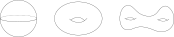
\includegraphics[width=.75\linewidth]{pics/chap8.pdf}
    \caption{Orientable surfaces}
    \label{fig:Orientable-surfaces}
  \end{figure}

  Non-orientable surfaces: $\B{RP}^2$, Klein's bottle, etc. See e.g. [Hirsch], [Massey].
  In dimension 3, one meets a famous open problem: the Poincare conjecture, which
  asserts that every compact topological 3-manifold that is homotopy equivalent to
  53 is homeomorphic to $S^3$. It is known that every topological 3-manifold $M^3$
  has a smooth structure $\C{A}$ and that two homeomorphic smooth 3-manifolds also
  are diffeomorphic. In the mid 1950s J. Milnor discovered smooth 7-manifolds
  that are homeomorphic to $S^7$, but not diffeomorphic to $S^7$. In collaboration with
  M. Kervaire he classified such exotic n-spheres. For example they showed that
  there are exactly 28 oriented diffeomorphism classes of exotic 7-spheres. In 1960
  Kervaire described a topological 10-manifold that has no smooth structure. During
  the 1960s the so-called ``surgery'' technique was developed, which in principle
  classifies all manifolds of a specified homotopy type, but only for $n\ge 5$.

  In the early 1980s M. Freedman completely classified the simply-connected compact 
  topological 4-manifolds; see [Freedman-Quinn]. At the same time S. Donaldson proved 
  some very surprising results about smooth compact 4-manifolds, which showed that there 
  is a tremendous difference between smooth and topological 4-manifolds. Donaldson used 
  methods originating in mathematical physics(Yang-Mills theory). This has led to a wealth of 
  new results on smooth 4-manifolds; see [Donaldson-Kronheimer].

  One of the most bizarre conclusions of the work of Donaldson and Freedman is
  that there exists a smooth structure on $\RR^4$ such that the resulting smooth 4-manifold
  `$`\RR^4$'' is not diffeomorphic to the usual $\RR^4$. It was proved earlier by S. Smale that
  every smooth structure on $\RR^n$ for $n\neq 4$ is diffeomorphic to the standard $\RR^n$.
\end{remark}
\chapter{Differential Forms on Smoth Manifolds}
\chapter{Integration on Manifolds}
Let $M^n$ be an oriented $n$-dimensional smooth manifold. We define an integral
\begin{align*}
  \int_M: \Omega^n_c(M^n)\to \RR
\end{align*}

on the vector space of differential $n$-forms with compact support. Next we shall
consider integration on subsets of $M^n$, and Stokes' theorem will be proved.
Finally we calculate $H^n (M^n)$ for an arbitrary orientable compact connected
smooth manifold $M^n$.

In the special case where $M^n = \RR^n$ (with the standard orientation) we can write
$\omega\in\Omega^n_c(\RR^n)$ in the form 
\begin{align*}
  \omega = f(x)\dd x_1\wedge\cdots\wedge\dd x_n,
\end{align*}

where $f\in C^\infty(\RR^n, \RR)$ has compact support. We then define 
\begin{align*}
  \int_{\RR^n}^{}{f(x)\dd x_1\wedge\cdots\wedge\dd x_n }
  = \int_{\RR^n} f(x)\dd \mu_n
\end{align*}

where $\dd\mu_n$ is the usual Lebesgue measure on $\RR^n$. The same definition can be used
when $\omega\in\Omega^n_c(V)$ for an open set $V\sseq\RR^n$, since $\omega$ and $f$ are smoothly 
extendable to the whole of $\RR^n$ by setting them equal to 0 on $\RR^n-\R{supp}_V(\omega)$.


\begin{lemma}\label{lemma:10-1}
  Let $\phi:V\to W$ be a diffeomorphism between open subsets $V$ and $W$ of $\RR^n$, and 
  assume that we the Jacobi determinant $\det (D_x\phi)$ is of constant sign $\delta=\pm 1$
  for $x\in V$. For $\omega\in \Omega^n_c(W)$ we have that 
  \begin{align*}
    \int_V \phi^*(\omega) = \delta\cdot\int_W \omega.
  \end{align*}
\end{lemma}

\begin{proof}
  If $\omega$ is written in the form 
  \begin{align*}
    \omega = f(x)\dd x_1\wedge\cdots\wedge\dd x_n
  \end{align*}
  with $f\in C_c^\infty(W, \RR)$, it follows from Example \ref{example:3-13}.(ii) that
  \begin{align*}
    \phi^*(\omega)
    & = f(\phi(x))\det(D_x\phi)\dd x_1\wedge\cdots\wedge\dd x_n\\ 
    & = \delta f(\phi(x))|\det(D_x\phi)|\dd x_1\wedge\cdots\wedge\dd x_n.
  \end{align*}

  The assertion follows from the transformation theorem for integrals which states that
  \begin{align*}
    \int_W f(x)\dd\mu_n 
    = \int_V f(\phi(x))|\det(D_x\phi)|\dd\mu_n.
  \end{align*}
\end{proof}

\begin{proposition}\label{prop:10-2}
  For an arbitrary oriented n-dimensional smooth manifold $M^n$ there exists a unique linear map
  \begin{align*}
    \int_M: \Omega^n_c(M^n)\to \RR
  \end{align*}
  with the following properties: If $\omega\in\Omega_c^n(M^n)$ has support contained in $U$, 
  where $(U, h)$ is a positively oriented $C^\infty$-chart, then 
  \begin{align}\label{eq:10-1}
    \int_M \omega = \int_{h(U)} h^{-1}(\omega)^*.
  \end{align}
\end{proposition}

\begin{proof}
  First consider $\omega\in \Omega^n_c(M^n)$ with ``small'' support, i.e. such that $\supp_M(\omega)$
is contained in a coordinate patch. Then $(U, h)$ can be chosen as above and
the integral is determined by \eqref{eq:10-1}. We must show that the right-hand side is
independent of the choice of chart. Assume that $(\tilde{U}, \tilde h)$ is another positively
oriented $C^\infty$-chart with $\supp_M(\omega)\sseq \tilde{U}$.

The diffeomorphism $\phi:V\to W$ from $V=h(U\cap \tilde{U})$ to $W=\tilde{h}(U\cap \tilde{U})$ given 
by $\phi=\tilde{h}\circ h^{-1}$ has everywhere positive Jacobi determinant. Since 
\begin{align*}
  \supp_{h(U)}((h^{-1})^*(\omega))\sseq V, && 
  \supp_{\tilde{h}(\tilde{U})}((\tilde{h}^{-1})^*(\omega))\sseq W,
\end{align*}
and $\phi^*(\tilde{h}^{-1})^*(\omega) = (h^{-1})^*(\omega)$, Lemma \ref{lemma:10-1} shows that 
\begin{align*}
  \int_{h(u)} (h^{-1})^*(\omega) = \int_{\tilde{h}(\tilde{U})} (\tilde{h}^{-1})^*(\omega).
\end{align*}
So for $\omega\in\Omega_c^n(M)$ with ``small'' support the integral defined by \eqref{eq:10-1} is independent
of the chart.

Now choose a smooth partition of unity $(\rho_\alpha)_{\alpha\in A}$ on $M$ subordinate to an 
oriented $C^\infty$-atlas on $M$. For $\omega\in\Omega_c^n(M)$ we have that 
\begin{align*}
  \omega = \sum_{\alpha\in A} \rho_\alpha\omega,
\end{align*}

where every term $\rho_\alpha\omega\in\Omega^n_c(M)$ has ``small'' support, and where only 
finitly many terms are non-zero. We define 
\begin{align*}
  I(\omega) = \sum_{\alpha\in A} \int_M \rho_\alpha\omega,
\end{align*}

where the term associated to $\alpha\in A$ is given by \eqref{eq:10-1}, applied to a $U_\alpha$ with
$\supp_M(\rho_\alpha)\sseq U_\alpha$. It is obvious that $I$ is a linear operator on $\Omega^n_c(M)$. If, in
particular, $\supp_M(\omega)\sseq U$, where $(U, h)$ is a positively oriented $C^\infty$-chart, the
terms of the sum can be calculated by \eqref{eq:10-1}, applied to $(U, h)$. This yields
\begin{align*}
  I(\omega) = \int_M \omega,
\end{align*}

which shows that $I$ is a linear operator with the desired properties. Uniqueness
follows analogously.
\end{proof}

\begin{lemma}\label{lemma:10-3}\;\par 
  \begin{enumerate}[(i)]
    \item $\int_M\omega$ changes sign when the orientation of $M^n$ is reversed.
    \item If $\omega\in\Omega^n_c(M^n)$ has support contained in an open set $W=\subset M^n$, then 
      \begin{align*}
        \int_M\omega = \int_W\omega,
      \end{align*}
      where $W$ is the orientation induced by $M$.
    \item If $\phi:N^n\to M^n$ is an orientation persevering diffeomorphism, then we have that 
      \begin{align*}
        \int_M\omega = 
        \int_N\phi^*(\omega)
      \end{align*}
      for $\omega\in\Omega^n_c(M)$.
  \end{enumerate}
\end{lemma}

\begin{proof}
  By a partition of unity, we can restrict ourselves to the case where
$\supp_M(\omega)$ is contained in a coordinate patch. All three properties are now easy
consequences of Lemma \ref{lemma:10-1} and \eqref{eq:10-1}.
\end{proof}

\begin{remark}\label{remark:10-4}
  In the above we could have considered integrals of continuous
  $n$-forms with compact support on $M^n$. If the orientation of $M$ is given by the
  orientation form $\sigma\in\Omega^n(M)$, a continuous $n$-form can be written uniquely as
  $f\sigma$, where $f\in C^0(M, \RR)$. The support of $f\sigma$ is equal to the support of $f$. The
  integral of \eqref{eq:10-1} extended to continuous $n$-forms gives rise to a linear operator
  \begin{align*}
    I_\sigma: C^n_c(M, \RR)\to \RR; && 
    I_\sigma(f) = \int_M f\sigma.
  \end{align*}
  This linear operator is positive, i.e. $I_\sigma(f)\ge 0$ for $f\ge 0$. By a partition of unity 
  it is sufficient to show this when $\supp(f)\sseq U$, where $(U, h)$ is a positive oriented $C^\infty$-chart.
  Then we have that 
  \begin{align*}
    I_\sigma(f) = \int_{h(U)} f\circ h^{-1}(x)\phi(x)\dd \mu_n,
  \end{align*}
  where $\phi$ is determined by $(h^{-1})^*(\sigma) = \phi(x)\dd x_1\wedge\cdots\wedge\dd x_n$. Since 
  $\phi$ is positive we get $I_\sigma(f)\ge 0$.

  According to Riesz's representation theorem (see for instance chapter 2 of [Rudin])
  $I_\sigma$ determines a positive measure $\mu_\sigma$ on $M$ which satisfies
  \begin{align*}
    \int_M f(x)\dd\mu_\sigma = \int_M f\sigma, \qquad f\in C^n_c(M, \RR).
  \end{align*}
  The entire Lebesgue integration machinery now becomes available, but we shall
  use only very little of it in the following.

  If $M^n$ is an oriented Riemannian manifold, the volume form $\R{vol}_M$ will determine
  a measure $\mu_M$ on $M^n$ analogous to the Lebesgue measure on $\RR^N$. For a compact
  set $K$ the volume of $K$ can be defined by
  \begin{align*}
    \R{vol}(K) = \int_K \R{vol}_M \in \RR.
  \end{align*}
\end{remark}

\begin{definition}\label{def:10-5}
  Let $M^n$ be a smooth manifold. A subset $N\sseq M^n$ is called a
domain with smooth boundary or a codimension zero submanifold with boundary,
if for every $p\in M$ there exists a $C^\infty$-chart $(U, h)$ around $p$, such that
\begin{align}\label{eq:10-2}
  h(U\cap N) = h(U)\cap \RR^n_-.
\end{align}
where $\RR^n_- = \{(x_1, \cdots x_n)\in\RR^n\mid x_1\le 0\}$. 
\end{definition}

Note that \eqref{eq:10-2} is automatically satisfied when $p$ is an interior or an exterior point
of $N$ (one can choose $(U, h)$ with $p\in U$, such that $h(U)$ is contained in an open
half-space in IRn defined by either $x_1 < 0$ or $x_1 > 0$). If $p$ is a boundary point of
$N$ then $h(p)$ has first coordinate equal to zero. Let $(U, h)$ and $(V, k)$ be smooth
charts around a boundary point $p\in \partial N$. The resulting transition diffeomorphism
\begin{align*}
  \phi = k\circ h^{-1}: h(U\cap V)\to k(U\cap V)
\end{align*}

induces a map 
\begin{align*}
  h(U\cap V)\cap \RR^n_- \to k(U\cap V)\cap \RR^n_-,
\end{align*}

which restricts to a diffeomorphism
\begin{align*}
  \Psi:h(U\cap V)\cap \partial\RR^n_-\to k(U\cap V)\cap \partial\RR^n_-.
\end{align*}

The Jacobi matrix at the point $q=h(p)\in\partial\RR^n_-$ for $\phi=(\phi_1, \cdots, \phi_n)$ 
has the form 
\begin{align*}
  D_q\phi = \begin{pmatrix}
    \frac{\partial \phi_1}{\partial x_1}(q) & 0 & \cdots & 0\\
    * \\
    \vdots & & D_q\Psi & \\
    * \\
  \end{pmatrix}
\end{align*}

We must have $\partial\phi_1/\partial x_1(q)\neq 0$, as $D_q\phi$ is invertible. Since $\phi$ maps 
$\RR^n_-$ into $\RR^n_-$, we have that $\partial\phi_1/\partial x_1(q)>0$.

A tangent vector $w\in T_pM$ at a boundary point $p\in\partial N$ is said to be outward
directed, if there exists a $C^\infty$-chart $(U, h)$ around p with $h(U\cap N) = h(U)\cap\RR^n_-$
and such that $D_ph(w)\in\RR^n$ has a positive first coordinate. This will then also be
the case for any other smooth chart around $p$.

\begin{lemma}\label{lemma:10-6}
  Let $N\sseq M^n$ be a domain with smooth boundary. Then $\partial N$ is an $(n - 1)$-dimensional 
  smooth submanifold of $M^n$.

  Suppose $M^n (n\ge2)$ is oriented. There is an induced orientation of $\partial N$ with the
  following property: if $p\in\partial N$ and $v_1\in T_pM$ is an outward directed tangent\index{outward directed tangent vector}
  vector then a basis $v_2,\cdots.v_n$ for $T_p\partial N$ is positively oriented if and only if 
  the basis $v_1,v_2,\cdots,v_n$ for $T_pM$ is positively oriented.
\end{lemma}

\begin{proof}
  Every smooth chart $(U, h)$ in $M$ that satisfies $h(U\cap N) = h(U)\cap\RR^n_-$ can
be restricted to a chart $(U\cap\partial N, h_|)$ on $\partial N$:
\begin{align*}
  h_|: U\cap\partial N\to h(U)\cap\partial\RR^n_-.
\end{align*}

These charts have mutual smooth overlap according to the above. This yields a
smooth atlas on $\partial N$.

Suppose $M^n$ is oriented. Then, possibly changing the sign of $x_2$, we can choose
a positively oriented chart $(U, h)$ of the considered type around any $p\in\partial N$. The
resulting smooth charts $(U\cap\partial N, h_|)$ on $\partial N$ have positively oriented 
transformation diffeomorphisms, and they determine an orientation of $\partial N$ that satisfies 
the stated property.
\end{proof}


\begin{remark}\label{remark:10-7}\;\par 
  \begin{enumerate}[(i)]
    \item We want to integrate $n$-forms $\omega\in\Omega_c^n(M)$ over domains $N$ with smooth
      boundary. In view of Remark $\ref{remark:10-4}$ we can set
      \begin{align*}
        \int_N\omega = \int_M 1_N\omega
      \end{align*}
      where $1_N$ is the function with value I on $N$ and zero outside $N$.
      Alternatively, one can prove an extension of Lemma \ref{lemma:10-1} which uses
      the following version of the transformation theorem: Let $\phi:V\to W$ be
      a diffeomorphism of open sets in $\RR^n$ that maps $\RR^n_-\cap V$ to $\RR^n_-\cap W$, 
      and let $f$ be a smooth function on $W$ with compact support. Then
      \begin{align*}
        \int_{\RR^n_-\cap W} d(x)\dd\mu_n 
        = \int_{\RR^n_-\cap V} f\phi(x) |\det(D_x\phi)|\dd\mu_n.
      \end{align*}
      (One could approximate both integrals by integrals over $W$ and $V$ upon
      multiplying $f$ by a sequence of smooth functions $\psi_i$ with values in $[0, 1]$
      and converging to $1_{\RR^n_-}$)
    \item In the case $n = 1$, Lemma \ref{lemma:10-6} holds in the following modified form. An
      orientation of $\partial N$ consists of a choice of sign, + or -, for every point
      $p\in\partial N$. Let $v_1\in T_pM$ be outward directed. Then $p$ is assigned the sign
      + if $v_1$ is a positively oriented basis of $T_pM$, otherwise the sign is -.
  \end{enumerate}
\end{remark}

A 0-form on $\partial N$ is a function $f:\partial N\to\RR$. When $f$ has compact support we define 
\begin{align*}
  \int_{\partial N} f = \sum_{p\in\partial N} \R{sgn}(p) f(p).
\end{align*}

These conventions are used in the case $n = 1$ of Stokes' theorem below.
\begin{figure}[!htb]
  \centering
  \includegraphics[width=.65\linewidth]{pics/chap10-1-o.pdf} 
  % \caption{}
  \label{fig:10-1}
\end{figure}

\begin{theorem}[Stokes' theorem]\label{theorem:10-8}\index{Stokes' Theorem}
  Let $N\sseq M^n$ be a domain with smooth boundary in an oriented smooth manifold. Let $\partial N$
  have induced orientation. For every $\omega\in\Omega^{n-1}(M)$ with $M\cap \supp_M(\omega)$ compact
  we have 
  \begin{align*}
    \int_{\partial N} i^*(\omega) = \int_N \dd\omega,
  \end{align*}
  where $i:\partial N\to M$ is the inclusion map.
\end{theorem}

\begin{proof}
  We assume that $n\ge 2$ and leave it to the reader to make the necessary
  changes for the case $n = 1$.

  It is clear that $i^*(\omega)$ has compact support. We can choose $f\in\Omega^0_c(M)$ with value
  constantly equal to 1 on $N\cap\supp_M(\omega)$. Since $f\omega$ coincides with $\omega$ on $N$, 
  both integrals are unchanged when $\omega$ is replaced by $f(\omega)$, so we may assume that $omega$
  has compact support.

  Choose a smooth atlas on $M$ consisting of charts of the type of Definition \ref{def:10-5}
  and a subordinate smooth partition of unity $(\rho\alpha)_{\alpha\in A}$. The formulas
  \begin{align*}
    \int_{\partial N}\omega = \sum_{\alpha} \int_{\partial N} 
    &&
    \int_N \dd\omega = \sum_{\alpha} \int_N \dd(\rho_\alpha\omega)
  \end{align*}

  reduce the problem to the case where $\omega\in\Omega^n_c(M)$. $\supp_M(\omega)\sseq U$
  and $(U, h)$ is a smooth chart $h(U\cap N) = h(U)\cap\RR^n_-$. Furthermore the chart $(U, h)$
  is assumed to be positively oriented.

  Let $\kappa\in\Omega^{n-1}_c(\RR^n)$ be the $(n-1)$-form that is $(h^{-1})^*(\omega)$ on 
  $h(U)$ and 0 on the rest of $\RR^n$. By diffeomorphism invariance we then have that 
  \begin{align*}
    \int_{\partial N}\omega 
      = \int_{h(U)\cap \partial\RR^n_-} (h^{-1})^*(\omega) 
      = \int_{\RR^n_-} \kappa
  \end{align*}
  and 
  \begin{align*}
    \int_N \dd\omega
      = \int_{h(U)\cap \RR^n_-} (h^{-1})^* \dd(\omega) 
      = \int_{\RR^n_-} \dd\kappa.
  \end{align*}
  Hence the proof reduces to the special case where $M=\RR^n, N=\RR^n_-$ and 
  $\omega\in\Omega_c^{n-1}(\RR^n)$. This case treated by direct calculation. We define 
  \begin{align*}
    \omega = \sum_{i=1}^{n }{f_i(x)\dd x_1\wedge\cdots\wedge\widehat{\dd x_i}\wedge\cdots\wedge\dd x_n},
  \end{align*}
  and choose $b>0$ such that $\supp_{\RR^n}f_i \sseq [-b, b]^n, 1\le i\le n$. Using Theorem \ref{theorem:3-12},
  \begin{align*}
    \omega_{|\partial\RR^n_-}
    = f_1(0, x_2, \cdots, x_n)\dd x_2\wedge\cdots\wedge\dd x_n.
  \end{align*}
  Hence 
  \begin{align}\label{eq:10-3}
    \int_{\partial\RR^n_-}\omega 
    = \int f_1(0, x_2, \cdots, x_n)\dd\mu_{n-1}.
  \end{align}
  By Theorem \ref{theorem:3-7} we have 
  \begin{align*}
    \dd\omega 
    = \sum_{i=1}^{n}{(-1)^{i-1}\frac{\partial f_i}{\partial x_i}\dd x_1\wedge\cdots\wedge\dd x_n}.
  \end{align*}
  Hence 
  \begin{align}\label{eq:10-4}
    \int_{\RR^n_-}
    = \sum_{i=1}^{n}{(-1)^{i-1}\int_{\RR^n_-}\frac{\partial f_i}{\partial x_i}\dd\mu_n}.
  \end{align}
  For $2\le i\le n$ we get 
  \begin{align*}
    & \int_{-\infty}^\infty \frac{\partial f_i}{\partial x_i}(x_1, \cdots, x_{i-1}, t, x_{i+1}, \cdots, x_n)\dd t \\
    = & f_i(x_1, \cdots, x_{i-1}, b, x_{i+1}, \cdots, x_n) 
      - f_i(x_1, \cdots, x_{i-1}, -b, x_{i+1}, \cdots, x_n).\\
    = & 0
  \end{align*}
  and then by Fubini's theorem
  \begin{align}\label{eq:10-5}
    \int_{\RR^n_-}\frac{\partial f_i}{\partial x_i}\dd\mu_n = 0\qquad (2\le i\le n).
  \end{align}
  When $i=1$, one gets 
  \begin{align*}
    \int_{-\infty}^0 \frac{\partial f_1}{\partial x_1}(t, x_2, \cdots, x_n)\dd t
    & = f_1(0, x_2, \cdots, x_n) - f_1(-b, x_2, \cdots, x_n)\\
    & = f_1(0, x_2, \cdots, x_n),
  \end{align*}
  and by Fubini's theorem 
  \begin{align}\label{eq:10-6}
    \int_{\RR^n_-} \frac{\partial f_1}{\partial x_1}\dd\mu_n
      = f_1(0, x_2, \cdots, x_n)\dd\mu_{n-1}.
  \end{align}
  By combining Equations \eqref{eq:10-3}--\eqref{eq:10-6} the desired formula follows.
\end{proof}

Taking $N = M$ in Theorem \ref{theorem:10-8} we have
\begin{corollary}\label{corollary:10-9}
  If $M^n$ is an oriented smooth manifold and $\omega\in\Omega^{n-1}_c(M)$ then 
  $\int_M\dd\omega=0$.
\end{corollary}

\begin{remark}\label{remark:10-10}
  Let $\omega$ be a closed $d$-form on $M^n$. One way of showing that the Cohomology class $[\omega]\in H^d(M)$
  is non-zero is to show that 
  \begin{align}\label{eq:10-7}
    \int_Q f^*(\omega) \neq 0
  \end{align}
  for a suitably chosen smooth map $f:Q^d\to M$ from a $d$-dimensional compact
  oriented smooth manifold $Q^d$. If $\omega=d\tau$ for some $\tau\in\Omega^{d-1}(M)$, then 
  Corollary \ref{corollary:10-9} yields
  \begin{align*}
    \int_Q f^*(\omega) = \int_Q \dd(f^*(\tau)) = 0.
  \end{align*}
  This, in essence, was the strategy from Examples \ref{example:1-2} and \ref{example:1-7}. It can 
  be shown (albeit in a very indirect way via cobordism theory) that $[\omega]=0$ if and only if
  all integrals of the form of \ref{eq:10-7} vanish.
\end{remark}


\begin{example}\label{example:10-11}
  In Example \ref{example:9-18} we considered the closed $(n -1)$-form on $\RR^n-\{0\}$,
  \begin{align*}
    \omega = \frac{1}{\|x\|^n} \sum_{i=1}^{n }{(-1)^{i-1}x_i\dd x_1\wedge\cdots\wedge\widehat{\dd x_i}\wedge\cdots\wedge\dd x_n}.
  \end{align*}
  Since the pre-image of $\omega$ under the inclusion of $S^{n-1}$ is the volume form $\R{vol}_{S^{n-1}}$,
  which has positive integral over $S^{n-1}$, we can conclude from Remark \ref{remark:10-10} that
  $[\omega]\neq 0$ in $H^{n-1} (\RR^n -\{0\})$. If $n\ge 2$ then, by Theorem \ref{theorem:6-13}, $[\omega]$ 
  is a basis of $H^{n-1} (\RR^n -\{0\})$. We thus have an isomorphism
  \begin{align*}
    H^{n-1} (\RR^n -\{0\})\simee \RR\qquad (n\ge 2)
  \end{align*}
  defined by integration over $S^{n-1}$. The image of $[\omega]$ under this isomorphism is
  the volume
  \begin{align*}
    \R{Vol}(S^{n-1}) = \int_{S^{n-1}} \R{vol}_{S^{n-1}}.
  \end{align*}
\end{example}

\begin{example}\label{example:10-12}
  The volume of $S^{n-1}$ can be calculated by applying Stokes' theorem to $D^n$ with the 
  standard orientation of IRn and the $(n - 1)$-fonn on $\RR^n$ given by
  \begin{align*}
    \omega_0 = \sum_{i=1}^{n}{(-1)^{i-1}x_i \dd x_1\wedge\cdots\wedge\widehat{\dd x_i}\wedge\cdots\wedge\dd x_n}.
  \end{align*}
  Since $\omega_{0|S^{n-1}} = \R{vol}_{S^{n-1}}$ and $\dd\omega_0 = n\dd x_1\wedge\cdots\wedge\dd x_n$ we have that 
  \begin{align*}
    \R{Vol}(S^{n-1}) 
    = \int_{S^{n-1}}\omega_0
    = \int_{D^n}\dd\omega_0
    = n\R{Vol}(D^n).
  \end{align*}
  By induction on $m$ and Fubini's theorem, it can be shown that
  \begin{align*}
    \R{Vol}(D^{2m}) = \frac{\pi^{m}}{m!}, && 
    \R{Vol}(D^{2m+1}) = \frac{2^{2m+1}m!\pi^{m}}{(2m+1)!}.
  \end{align*}
  This yields
  \begin{align*}
    \R{Vol}(S^{2m-1}) = \frac{2\pi^{m}}{(m-1)!}, &&
    \R{Vol}(S^{2m}) = \frac{2^{2m+1}m!\pi^{m}}{(2m)!}.
  \end{align*}
\end{example}

We conclude this chapter with a proof of the following:

\begin{theorem}\label{theorem:10-13}
  If $M^n$ is a connected oriented smooth manifold, then the sequence
  \begin{align}\label{eq:10-8}
    \Omega^{n-1}_c(M)
    \xra[\dd] \Omega^n_c(M)
    \xra[\int_M] \RR
    \xra 0
  \end{align}
  is exact.
\end{theorem}

\begin{corollary}\label{corollary:10-14}
  For a connected compact smooth manifold $M^n$, integration over $M$ induces an isomorphism
  \begin{align*}
    \int_M: H^n(M^n)\xra[\simee] \RR.\tag*{\qedsymbol}
  \end{align*}
\end{corollary}

In \eqref{eq:10-8} it is obvious that the integral is non-zero and hence surjective. It follows
from Corollary \ref{corollary:10-9} that the image of $\dd$ is contained in the kernel of the 
integral. We show the converse inclusion.

\begin{lemma}\label{lemma:10-15}
  Theorem \ref{theorem:10-13} holds for $M=\RR^n, n\ge 1$.
\end{lemma}

\begin{proof}
  Let $\omega\in\Omega^n_c(\RR^n)$ be a diffeomorphism $n$-form with $\int_{\RR^n}\omega=0$. We must find 
  that $\kappa\in\Omega^{n-1}_c(\RR^n)$, such that $\dd\kappa=\omega$. We can write $\omega=f(\FF{x})\dd x_1 \wedge\cdots\wedge\dd x_n$,
  and let 
  \begin{align*}
    \kappa = \sum_{j=1}^{n }{(-1)^{i-1}f_j(\FF{x})\dd x_1\wedge\cdots\wedge\widehat{\dd x_j}\wedge\cdots\wedge\dd x_n}. 
  \end{align*}
  A simple calculation gives 
  \begin{align*}
    \dd\kappa = \left(\sum_{j=1}^{n}{\frac{\partial f_j}{\partial x_j}}\right)\dd x_1\wedge\cdots\wedge\dd x_n.
  \end{align*}
  Hence we need to prove the following assertion:\par 
  ($P_n$): Let $f\in C_c^\infty(\RR^n)$ be a function with $\int f(x)\dd\mu_n = 0$. There exsits functions
  $f_1, \cdots, f_n$ in $C_c^\infty(\RR^n)$ such that
  \begin{align*}
    \sum_{j=1}^{n}{\frac{\partial f_j }{\partial x_j }} = f.
  \end{align*}
  We prove ($P_n$) by induction. For $n=1$ we are given a smooth function $x\in C_c^\infty(\RR)$ 
  with $\int_{-\infty}^\infty f(t)\dd t = 0$. The problem is solved by setting 
  \begin{align*}
    f_1(x) = \int_{-\infty}^x f(t)\dd t.
  \end{align*}
  Assume that ($P_{n-1}$) for $n\ge 2$, and let $f\in C_c^\infty(\RR^n, \RR)$ be a function with $\int f(x)\dd\mu_n = 0$.
  We choose $C>0$ with $\supp(f)\sseq [-C, C]^n$ and define 
  \begin{align}\label{eq:10-9}
    g(x_1, \cdots, x_{n-1}) = \int_{-\infty}^{\infty} f(x_1, \cdots, x_{n-1}, x_n)\dd x_n.
  \end{align}
  (The limits can be be replaced by $-C$ and $C$, respectively). The function $g$ is smooth, 
  since we can differentiate under the integral sign. Furthennore $\supp(g)\sseq [-C, C]^{n-1}$. 
  Fubini's theorem yields $\int g\dd\mu_{n-1} = \int f\dd\mu_n = 0$. Using $(P_{n-1})$ we get functions 
  $g_1, \cdots, g_{n-1}$ in $C_c^\infty(\RR^{n-1}, \RR)$ with 
  \begin{align}\label{eq:10-10}
    \sum_{j=1}^{n-1}{\frac{\partial g_j}{\partial x_j}} = g.
  \end{align}
  We choose a function $\rho\in C_c^\infty(\RR, \RR)$ with $\int_{-\infty}^\infty \rho(t)\dd t = 1$, and 
  define $f_j\in C_c^\infty(\RR^n, \RR)$,
  \begin{align}\label{eq:10-11}
    f_j(x_1, \cdots, x_n) = g_j(x_1, \cdots, x_{n-1})\rho(x_n), 1\le j\le n-1.
  \end{align}
  Let $h\in C_c^\infty(\RR, \RR)$ be the function
  \begin{align}\label{eq:10-12}
    h = f - \sum_{j=1}^{n-1}{\frac{\partial f_j}{\partial x_j}}.
  \end{align}
  A function $f_n \in C_c^\infty(\RR^n)$ with $\partial f_n/\partial x_n=h$ is given by
  \begin{align}\label{eq:10-13}
    f_n(x_1, \cdots, x_{n-1}, x_n) = \int_{-\infty}^{x_n} h(x_1, \cdots, x_{n-1}, t)\dd t.
  \end{align}

  It is obvious that $f_n$ is smooth, but we must show that it has compact support. To
  this end it is sufficient to show that the integral of \eqref{eq:10-13} vanishes when the upper
  limit X n is replaced by 00. Now \eqref{eq:10-10}, \eqref{eq:10-11} and \eqref{eq:10-12} yield 
  that
  \begin{align*}
    h(x_1, \cdots, x_{n-1}, x_n) 
    & = f(x_1, \cdots, x_{n-1}, t) - \sum_{j=1}^{n-1}{\frac{\partial g_j}{\partial x_j}}\rho(t)\\
    & = f(x_1, \cdots, x_{n-1}, t) - g(x_1, \cdots, x_{n-1})\rho(t).
  \end{align*}
  Finally from \eqref{eq:10-10} it follows that 
  \begin{align*}
    & \int_{-\infty}^\infty h(x_1, \cdots, x_{n-1}, t)\dd t \\
    = & \int_{-\infty}^\infty f(x_1, \cdots, x_{n-1}, t)\dd t 
      - g(x_1, \cdots, x_{n-1})\int_{-\infty}^\infty \rho(t)\dd t\\
    = & 0.
  \end{align*}
\end{proof}

\begin{lemma}\label{lemma:10-16}
  Let $(U_\alpha)_{\alpha\in A}$ be an open cover of the connected manifold $M$, and 
  let $p, q\in M$. There exists indices $\alpha_1, \cdots, \alpha_k$ such that 
  \begin{enumerate}[(i)]
    \item $p\in U_\alpha$ and $q\in U_{\alpha_k}$.
    \item $U_{\alpha_i}\cap U_{\alpha_{i+1}}\neq\ns$ for $1\le i\le k-1$.
  \end{enumerate}
\end{lemma}

\begin{proof}
  For a fixed $p$ we define $V$ to be the set of $q\in M$, for which there exists
a finite sequence of indices $\alpha_1, \cdots, \alpha_k$ from $A$, such that (i) and (ii) are 
satisfied. It is obvious that $V$ is both open and closed in $M$ and that $V$ contains $p$. Since
$M$ is connected, we must have $V = M$.
\end{proof}

\begin{lemma}\label{lemma:10-17}
  Let $U\sseq M$ be an open set diffeomorphic to $\RR^n$ and let $W\sseq U$ be 
  non-empty and open. For every $\omega\in\Omega^n_c(M)$ with $\supp_M(\omega)\sseq U$, there 
  exists a $\kappa\in\Omega^{n-1}_c(M)$ such that $\supp\kappa\sseq U$ and $\supp(\omega-\dd\kappa)\sseq W$.
\end{lemma}

\begin{proof}
  It suffices to prove the lemma when $M = U$, and by diffeomorphism
invariance it is enough to consider the case where $M = U = \RR^n$. Choose $\omega_1\in\Omega_c^n(\RR^n)$
with $\supp(\omega_1)\sseq W$ and $\int_{\RR^n}\omega_1 = 1$. Then 
\begin{align*}
  \int_{\RR^n} (\omega -a\omega_1) = 0, \qquad \text{ where } a = \int_{\RR^n}\omega.
\end{align*}

By Lemma \ref{lemma:10-15} we can find a $\kappa\in\Omega^{n-1}_c(\RR^n)$ with 
\begin{align*}
  \omega - a\omega_1 = \dd\kappa.
\end{align*}
Hence $\omega - \dd\kappa = \dd\omega_1$ has its support in $W$.
\end{proof}

\begin{lemma}\label{lemma:10-18}
  Assume that $M^n$ is connected and let $W\sseq M$ be non-empty and 
  open. For every $\omega\in\Omega^n_c(M)$ there exists a $\kappa\in\Omega^{n-1}_c(M)$ with 
  $\supp(\omega-\dd\kappa)\sseq W$.
\end{lemma}

\begin{proof}
  Suppose that $\supp\omega\sseq U_1$ for some open set $U_1\sseq M$ diffeomorphic to 
  $\RR^n$. We apply Lemma \ref{lemma:10-16} to find open sets $U_2, \cdots, U_k$, diffeomorphic 
  to $\RR^n$, such that $U_{i-1}\cap U_i\neq \ns$ for $2\le i\le k$ and $U_k\sseq W$. We use Lemma 
  \ref{lemma:10-17} to successively choose $\kappa_1, \cdots, \kappa_{k-1}$ in $\Omega^{n-1}_c(M)$ such that 
  \begin{align*}
    \supp\left(\omega - \sum_{i=1}^{j }{\dd\kappa_i }\right)
    \sseq U_j\cap U_{j+1}\qquad (1\le j\le k-1).
  \end{align*}

  The lemma holds for $\kappa = \sum_{i=1}^{k-1}{\kappa_i}$.

  In the general case we use a partition of unity to write
  \begin{align*}
    \omega = \sum_{j = 1}^{m }{\omega_j},
  \end{align*}
  where $\omega_j\in\Omega^n_c(M)$ has support contained in a open set diffeomorphic to $\RR^n$. 
  The above gives $\tilde{\kappa}_j\in\Omega^{n-1}_c(M), 1\le j\le m$, such that $\supp(\omega_j-\dd\tilde{\kappa_j})\sseq W$.
  For 
  \begin{align*}
    \tilde{\kappa} = \sum_{j=1}^{m }{\tilde{\kappa}_j} \in \Omega^{n-1}_c(M)
  \end{align*}
  we have that
  \begin{align*}
    \omega -\dd\tilde{\kappa} = \sum_{j=1}^{m }{(\omega_j - \dd\tilde{\kappa}_j)}
  \end{align*}
  Hence $\supp(\omega-\dd\tilde{\kappa})\sseq \cup_{j=1}^m\sseq W$.
\end{proof}

\textbf{Proof of Theorem \ref{theorem:10-13}.} Suppose given $\omega\in\Omega^n_c(M)$ with 
$\int_M\omega = 0$. Choose an open set $W\sseq M$ diffeomorphic to $\RR^n$. By Lemma \ref{lemma:10-18}
we can find a $\kappa\in\Omega_c^{n-1}\sseq W$. But then by Corollary \ref{corollary:10-9},
\begin{align*}
  \int_W (\omega - \dd\kappa) 
  = \int_M (\omega - \dd\kappa)
  = - \int_M\dd\kappa 
  = 0
\end{align*}

Lemma \ref{lemma:10-15} implies that Theorem \ref{theorem:10-13} holds for $W$, i.e. there 
exists a $\tau_0\in\Omega^{n-1}_c(W)$ that satisfies
\begin{align*}
  (\omega - \dd\kappa)_{|W} = \dd\tau_0.
\end{align*}

Let $\tau\in \Omega^{n-1}_c(M)$ be the extension of $\tau_0$ which vanishes outside $\supp_W(\tau_0)$.
Then $\omega -\dd\kappa=\dd\tau$, so $\tau+\kappa$ maps $\omega$ under $d$. \hfill\(\qedsymbol\)
\chapter{Degree, Linking Numbers and Index of Vector Fields}
Let $f:N^n\to M^n$ be a smooth map between compact connected oriented manifolds 
of the same dimension $n$. We have the commutative diagram
\begin{equation}\label{eq:11-1}
  \begin{tikzcd}
    H^n(M) \arrow[d, "\simee"']\rar{H^n(f)} & H^n(N)\arrow[d, "\simee"']\\
    \RR \rar{\R{deg}(f)} & \RR 
  \end{tikzcd}
\end{equation}

where the vertical isomorphisms are given by integration over $M$ and $N$ respectively; cf. 
Corollary \ref{corollary:10-14}. The lower horizontal arrow is multiplication by the
real number $\R{deg}(f)$ that makes the diagram commutative. Thus for $\omega\in\Omega^n(M)$,
\begin{align}\label{eq:11-2}
  \int_N f^*\omega = \R{deg}(f)\int_M \omega.
\end{align}

This formulation can be generalized to the case where $N$ is not connected:

\begin{proposition}\label{prop:11-1}
  Let $f:N^n\to M^n$ be a smooth map between compact $n$-dimensional oriented manifolds 
  with $M$ connected. There exists a unique $\R{deg}(f)\in\RR$ such that \eqref{eq:11-2} holds 
  for all $\omega\in\Omega^n(M)$. We call $\R{deg}(f)$ the degree of $f$.
\end{proposition}

\begin{proof}
  We write $N$ as a disjoint union of its connected components $N_1, \cdots, N_k$ and
and denote the restriction of $f$ to $N_j$ by $f_j$. We have already defined $\R{deg}(f_i)$;
we set
\begin{align}\label{eq:11-3}
  \R{deg}(f) = \sum_{j=1}^{k }{\R{deg}(f_j)}.
\end{align}

Thus for $\omega\in\Omega^n(M)$, we have, 
\begin{align*}
  \int_N f^*\omega 
  = \sum_{j=1}^{k}{\int_{N_j}f_j^*\omega} 
  = \sum_{j=1}^{k}{\R{deg}(f_j)\int_M\omega} 
  = \R{deg}(f)\int_M\omega.
\end{align*}
\end{proof}

\begin{corollary}\label{corollary:11-2}
  $\R{deg}(f)$ depends only on the homotopy class of $f:N\to M$.
\end{corollary}

\begin{proof}
  By \eqref{eq:11-3} we can restrict ourselves to the case where $N$ is connected.
The assertion then follows from diagram (1), since $H^n(f)$ depends only on the
homotopy class of $f$.
\end{proof}

\begin{corollary}\label{corollary:11-3}
  Suppose $N^n\xra[f]M^n\xra[g]P^n$ are smooth maps between $n$-dimensional compact 
  oriented manifolds and that $M$ and $P$ are connected. Then 
  \begin{align*}
    \R{deg}(gf) = \R{deg}(g)\R{deg}(f).
  \end{align*}
\end{corollary}

\begin{proof}
  For $\omega\in\Omega^n(P)$, 
  \begin{align*}
    \R{deg}(gf)\int_p\omega 
    & = \int_N(gf)^*(\omega)
      = \int_N f^*(g^*(\omega)) \\
    & = \R{deg}(f)\int_M g^*(\omega)
      = \R{deg}(f)\R{deg}(g)\int_P\omega.
  \end{align*}
\end{proof}

\begin{remark}\label{remark:11-4}
  If $f:M^n\to N^n$ is a smooth map of a connected compact orientable
manifold to itself then $\R{deg}(f)$ can be defined by chosing an orientation of $M$ and
using it at both the domain and range. Change of orientation leaves $\R{deg}(f)$.
unaffected.
\end{remark}

We will show that $\R{deg}(f)$ takes only integer values. This follows from an important geometric 
interpretation of $\R{deg}(f)$ which uses the concept of regular value. In general $p\in M$ is said 
to be a \Index{regular value} for the smooth map $f:N^n\to M^n$ if
\begin{align*}
  D_qf:T_pN\to T_pM
\end{align*}

is surjective for all $q\in f^{-1}(p)$. In particular, points in the complement of $f(N^n)$
are regular values. Regular values are in rich supply:

\begin{theorem}[Brown-Sard]\label{theorem:11-5}\index{Brown-Sard theorem}\index{Sard theorem}
  For every smooth map $f: N^n \to M^m$ the set of regular values is dense in $M^m$.
\end{theorem}

When proving Theorem \ref{theorem:11-5} one may replace $M^m$ by an open subset $W\sseq M$
diffeomorphic to $\RR^n$, and replace $N^n$ by $f^{-1}(W)$. This reduces Theorem \ref{theorem:11-5}
to the special case where $M^m = \RR^m$.

In this case one shows, that almost all points in $\RR^m$ (in the Lebesgue sense) are
regular values. By covering $N^n$ with countably many coordinate patches and
using the fact that the union of countably many Lebesgue null-sets is again a
null-set, Theorem \ref{theorem:11-5} therefore reduces to the following result:

\begin{theorem}[Sard, 1942]\label{theorem:11-6}
  Let $f:U\to\RR^m$ be a smooth map defined on an open set $U\sseq\RR^n$ and let
  \begin{align*}
    S = \{x\in U\big| \text{rank} D_xf < m\}.
  \end{align*}

  Then $f(S)$ is a Lebesgue null-set in $\RR^m$.
\end{theorem}

Note that $x\in U$ belongs to $S$ if and only if every $m\times m$ submatrix of the Jacobi
matrix of $f$, evaluated at $x$, has determinant zero. Therefore $S$ is closed in $U$ and
we can write $S$ as a union of at most countably many compact subsets $K\sseq S$.
Theorem \ref{theorem:11-6} thus follows if $f(K)$ is a Lebesgue null-set for every compact
subset $K$ of $S$. We shall only use and prove these theorems in the case $m = n$,
where they follow from

\begin{proposition}\label{prop:11-7}
  Let $f:U\to \RR^n$ be a $C^1$-map defined on an open set $U\sseq \RR^n$,
and let $K\sseq S$ be a compact set such that $\det(D_xf) = 0$ for all $x\in K$. Then
$f(K)$ is a Lebesgue null-set in $\RR^n$.
\end{proposition}

\begin{proof}
  Choose a compact set $L\sseq U$ which contains $K$ in the interior, $K\sseq L$. Let 
  $C>0$ be a constant such that 
  \begin{align}\label{eq:11-4}
    \sup_{\xi\in L}\|\grad_\xi f_j\| \leq C\qquad (1\le j \le n).
  \end{align}

  Here $f_j$ is the $i$-th coordinate function of $f$, and $\|\cdot\|$ denotes the Euclidean norm.
  Let 
  \begin{align*}
    T = \prod_{i=1}^n [t_i, t_i + a]
  \end{align*}

  be a cube such that $K\sseq S$, and let $\epsilon>0$. Since the functions $\partial f_j/\partial x_i$ 
  are uniformly continuous on $L$, there exists a $\delta >0$ such that
  \begin{align}\label{eq:11-5}
    \|x-y\|\le \delta \implies 
    \left|\frac{\partial f_j }{\partial x_i }(x) - \frac{\partial f_j }{\partial x_i}(y)\right|\le \epsilon,
    (1\le i,j\le n \text{ and } x, y\in L).
  \end{align}
  We subdivide $T$ into a union of $N^n$ closed small cubes $T_l$ with side length $\frac aN$,
  and choose $N$ so that
  \begin{align}\label{eq:11-6}
    \R{diam}(T_1) = \frac{a\sqrt{n}}{N}\le \delta, \qquad T_1\cap K \neq 0\implies T_1\sseq L.
  \end{align}
  For a small cube $T_l$ with $T_1\cap K\neq \ns$ we pick $x\in T_l\cap K$. If $y\in T_l$ the 
  mean value theorem yields points $\xi_j$ on the line segment between $x$ and $y$ for which
  \begin{align}\label{eq:11-7}
    f_j(y) - f_j(x) 
    = \sum_{i=1}^{n }{\frac{\partial f_j }{\partial x_i }(\xi_j)(y_i - x_i)}.
  \end{align}

  Since $\xi_j\in T_l\sseq L$, the Cauchy-Schwarz inequality and \eqref{eq:11-4} give
  \begin{align*}
    |f_j(y) - f_j(x)| \le C\|y-x\|
  \end{align*}
  and by \eqref{eq:11-6}, 
  \begin{align}\label{eq:11-8}
    \|f(y) - f(x)\| \le C\|y-x\| \le C\sqrt{n}\R{diam}(T_1) = \frac{anC}{N}.
  \end{align}
  Formula \eqref{eq:11-7} can be rewritten as
  \begin{align}\label{eq:11-9}
    f(y) = f(x) + D_x f(y-x) + z,
  \end{align}
  where $z = (z_1, \cdots, z_n)$ is given by 
  \begin{align*}
    z_j = \sum_{i=1}^{n }{\left(\frac{\partial f_j }{\partial x_i }(\xi_j) - \frac{\partial f_j }{\partial x_i }(x_i)\right) (y_i - x_i)}.
  \end{align*}
  By \eqref{eq:11-6}, $\|\xi_j-x\|\le \delta$, so that $|z_j|\le \epsilon n\frac aN$. Hence 
  \begin{align}\label{eq:11-10}
    \|z\| \le \epsilon \frac{an\sqrt{n}}{N}.
  \end{align}
  Since the image of $D_xf$ is a proper subspace of $\RR^n$, we may choose an affine
  hyperplane $H\sseq \RR^n$ with
  \begin{align*}
    f(x) + \im (D_xf)\sseq H.
  \end{align*}
  By \eqref{eq:11-9} and \eqref{eq:11-10} the distance from $f(y)$ to $H$ is less than $\epsilon \frac{an\sqrt{n}}{N}$. 
  Then \eqref{eq:11-8} implies that $f(T_l)$ is contained in the set $D_l$ consisting of all points $q\in\RR^n$ whose
  orthogonal projection $\R{pr}(q)$ on $H$ lies in the closed ball in $H$ with radius $\epsilon \frac{anC}{N}$
  and centre $f(x)$ and $\|q-\R{pr}(q)\|\le \epsilon \frac{an\sqrt{n}}{N}$. For the Lebesgue measure $\mu_n$ on $\RR^n$
  we have
  \begin{align*}
    \mu_n(D_i) 
      = 2\epsilon \frac{an\sqrt{n}}{N} \left(\frac{anC }{N }\right)^{n-1}
        \mkern-15mu\R{vol}(D^{n-1})
      = \epsilon \frac{c}{N^n}
  \end{align*}
  where $c = 2a^nn^{n+\frac12}C^{n-1}\R{Vol}(D^{n-1})$. For evry small cube $T_l$ with $T_l\cap K\neq\ns$
  we now have $\mu_n(f(T_l))\le \epsilon\frac{c}{N^n}$. Since there are at most $N^n$ such small cubes $T_l$,
  $\mu_n(f(K))\le c\epsilon$. This holds for every $\epsilon>0$ and proves the assertion.
\end{proof}

\begin{lemma}\label{lemma:11-8}
  Let $p\in M^n$ be a regular value for the smooth map $f:N^n\to M^n$, with $N^n$ compact. 
  Then $f^{-1}(p)$ consists offinitely many points $q_1, \cdots, q_k$. Moreover, there exist 
  disjoint open neighborhoods $V_i$ of $q_i$ in $N^n$, and an open neighborhood $U$ of $p$ in $M^n$,
  such that
  \begin{enumerate}[(i)]
    \item $f^{-1}(U) = \cup_{i=1}^k V_i$.
    \item $f_i$ maps $V_i$ diffeomorphically onto $U$ for $1\le i\le k$.
  \end{enumerate}
\end{lemma}

\begin{proof}
  For each $q\in F^{-1}(U)$, $D_qf:T_qN\to T_q M$ is an isomorphism. From the
inverse function theorem we know that $f$ is a local diffeomorphism around $q$. In
particular $q$ is an isolated point in $f^{-1}(p)$. Compactness of $N$ implies that $f^{-1}(p)$
consists of finitely many points $q_1, \cdots, q_k$. We can choose mutually disjoint open
neighborhoods $W_i$ of $q_i$ in $N$, such that $f$ maps $W_i$ diffeomorphically onto an
open neighborhood $f(W_i)$ of $p$ in $M$. Let
\begin{align*}
  U = \left(\bigcap_{i=1}^k f(W_i)\right)
    - f\left(N - \bigcup_{i=1}^k W_i\right) 
\end{align*}
Since $N - \bigcup_{i=1}^k W_i$ is closed in $N$ and therefore compact $f(N - \bigcup_{i=1}^k W_i)$ is 
also compact. Hence $U$ is an open neighborhood of $p$ in $M$. We then set 
$V_i = W_i\cap f^{-1}(U)$.
\end{proof}

Consider a smooth map $f:N^n\to M^n$ between compact $n$-dimensional oriented
manifolds, with $M$ connected. For a regular value $p\in M$ and $q\in f^{-1}(p)$, define
the local index
\begin{align}
  \R{Ind}(f, g) = \left\{\begin{aligned}
    & 1   && \text{ if } D_qf:T_pN \to T_pM \text{ preserves orientation } \\
    & -1  && \text{ otherwise. }
  \end{aligned}\right.
\end{align}

\begin{theorem}\label{theorem:11-9}
  In the situation above, and for every regular value $p$, 
  \begin{align*}
    \R{deg}(f) = \sum_{q\in f^{-1}(p)}{\R{Ind}(f; q)}.
  \end{align*}
  In particular $\R{deg}(f)$ is an integer. 
\end{theorem}

\begin{proof}
  Let $q_i, V_i$, and $U$ be as in Lemma \ref{lemma:11-8}. We may assume that $U$ and
hence $V_i$ connected. The diffeomorphism $f_{|V_i}:V_i\to U$ is positively or negatively
oriented, depending on whether $\R{Ind}(f; q)$ is 1 or -1. Let $\omega\in\Omega^n(M)$ be an
$n$-form with
\begin{align*}
  \supp_M(\omega)\sseq U, \qquad \int_M \omega = 1.
\end{align*}

Then $\supp_N(f^*(\omega))\sseq f^{-1}(U) = V_1\cup\cdots\cup V_k$, and we can write 
\begin{align*}
  f^*(\omega) = \sum_{i=1}^k{\omega_i}
\end{align*}
where $\omega_i\in\Omega^n(N)$ and $\supp(\omega_1)\sseq U$. Here $\omega_{i|V_i} = (f_{|V_i})^*(\omega_{|U})$. The 
formula is a consequence of the following calculation:
\begin{align*}
  \R{deg}(f) 
  & = \R{deg}(f)\int_M\omega 
    = \int_Mf^*(\omega) 
    = \sum_{i=1 }^{k }{\int_N \omega_i}
    = \sum_{i=1}^{k}{\int_{V_i} (f_{|V_i})^*(\omega_{|U})} \\
  & = \sum_{i=1 }^{k }{\R{Ind}(f; q_i)\int_U \omega_{|U} }
    = \sum_{i=1}^{k}{\R{Ind}(f; q_i)}.
\end{align*} 

In the special case where $f^{-l}(p) = 0$ the theorem shows that $\R{deg}(f) = 0$ (in the
proof above we get $f^*(\omega) = 0$). Thus we have 
\end{proof}

\begin{corollary}\label{corollary:11-10}
  If $\R{deg}(f)\neq 0$, then $f$ is surjective.
\end{corollary}

\begin{proposition}\label{prop:11-11}
  Let $F:P^{n+1}\to M^n$ be a smooth map between oriented smooth
  manifolds, with $M^n$ compact and connected. Let $X\sseq P$ be a compact domain with
  smooth boundary $N^n =\partial x$, and suppose $N$ is the disjoint union ofsubmanifolds
  $N_i^n,\cdots, N_k^n$. If $f_i = F_{|N_i}$, then
  \begin{align*}
    \sum_{i=1 }^{k }{\R{deg}(f_i)} = 0.
  \end{align*}
\end{proposition}

\begin{proof}
  Let $f = F_{|N}$ so that 
  \begin{align*}
    \R{deg}(f) = \sum_{i=1}^{k}{\R{deg}(f_i)}.
  \end{align*}
  On the other hand, if $\omega\in\Omega^n(M)$ has $\int_M \omega=1$, then 
  \begin{align*}
    \R{deg}(f) = \int_N f^*(\omega)
    = \int_X \dd F^*(\omega)
    = \int_X F^*(\dd\omega)
    = 0
  \end{align*}
  where the second equation is from Theorem \ref{theorem:10-8}.
\end{proof}

We shall give two applications of degree. We first consider linking numbers, and
then treat indices of vector fields.

\begin{definition}\label{def:11-12}\index{linking number}
  Let $J^d$ and $K^l$ be two disjoint compact oriented connected smooth submanifolds of $\RR^{n +1}$, 
  whose dimensions $d\ge 1, l\ge 1$ satisfy $d + l = n$. Their linking number is the integer
  \begin{align*}
    \R{lk}(J, K) = \R{deg}(\Psi_{J, K})
  \end{align*}
  where 
  \begin{align*}
    \Psi = \Psi_{J, K}:J\times K\to S^{n};\qquad \Psi(x, y) = \frac{y-x}{\|y-x\|}.
  \end{align*}
\end{definition}

Here $J\times K$ is equipped with the product orientation (cf. Remark \ref{remark:9-20}) and $S^n$ 
is oriented as the boundary of $D^{n+1}$ with the standard orientation of $\RR^{n+1}$. We note
that $\R{lk}(J, K)$ changes sign when the orientation of either $J$ or $K$ is reversed.

\begin{proposition}\label{prop:11-13}\;\par 
  \begin{enumerate}[(i)]
    \item $\R{lk}(K^l, J^d) = (-1)^{(d+1)(l+1)}\R{lk}(J^d, K^l)$.
    \item If $J$ and $K$ can be separated by a hyperplane $H\subset\RR^{n+1}$ then $\R{lk}(J, K) = 0$.
    \item Let $g_t$ and $h_t$ be homotopies of the inclusions $g_0:J\to\RR^{n+1}$ and $h_0:K\to\RR^{n+1}$
      to smooth embeddings $g_1$ and $h_1$, such that $g_t(J)\cap h_t(K) = \ns$ for all $t\in[0, 1]$. Then 
      $\R{lk}(J, K) = \R{lk}(g_1(J), h_1(K))$.
    \item Let $\Phi:P^{n+1}\to\RR^{n+1}-J$ be a smooth map with $P$ oriented. Given a compact domain 
      $R\sseq P$ with smooth boundary $\partial R$, let $Q_1, \cdots, Q_k$ be the connected components 
      of $\partial R$. Suppose each $\Phi_{|Q_j}$ is a smooth embedding. If $K_i = \Phi(Q_i)$, then 
      \begin{align*}
        \sum_{i=1 }^{k }{\R{lk}(J; K_i)} = 0.
      \end{align*}
  \end{enumerate}
\end{proposition}

\begin{proof}
  We look at the commutative diagram 
  \begin{center}
    \begin{tikzcd}
      J\times K \rar{\Psi_{J, K}}\dar{T} & S^n \dar{A}\\
      K\times J \rar{\Psi_{K, J}} & S^n
    \end{tikzcd}
  \end{center}

  where $T$ interchanges factors and $A$ is the antipodal map $Av = -v$. Then (i)
  follows from Corollary \ref{corollary:11-3} upon using that
  \begin{align*}
    \R{deg}(T) = (-1)^{dl}, \qquad \R{deg}(A) = (-1)^{n+1} = (-1)^{d+l+1}.
  \end{align*}

  In the situation of (ii) the image of $\Psi$ will not contain vectors parallel to $H$, and
  the assertion follows from Corollary \ref{corollary:11-10}.

  Assertion (iii) is a consequence of the homotopy property, Corollary \ref{corollary:11-2}. Indeed,
  a homotopy $J\times K\times [0,1]\to S^n$ is given by
  \begin{align*}
    (h_t(y) -g_t(x))\big/ \|h_t(y) - g_t(x)\|.
  \end{align*}
  Finally (iv) follows from Proposition \ref{prop:11-11} applied to the map $F: J\times P\to S^n$ with
  \begin{align*}
    F(x, y) = (\Phi(y) - x)\big/ \|\Phi(y) - x\|.
  \end{align*}
  and to the domain $X=J\times R$ with boundary components $I\times Q_i$. Indeed, 
  $f_i = E_{|J\times Q_i}$ has degree $\R{deg}(f_i) = \R{lk}(J, K_i)$.
\end{proof}

Here is a picture to illustrate (iv):
\begin{figure}[!htb]
  \centering
  \includegraphics[width=.4\linewidth]{./pics/chap11-1-o.pdf} 
  \caption{Figure 1}
  \label{fig:11-1}
\end{figure}

If $\R{lk}(J, K)\neq 0$ then (ii) and (iii) of Proposition \ref{prop:11-13} imply that $J$ 
and $K$ cannot be deformed to manifolds separated by a hyperplane.

We shall now specialize to the classical case of knots in $\RR^3$ where $J$ and $K$ are
disjoint oriented submanifolds of $\RR^3$ diffeomorphic to $S^1$. Let us choose smooth
regular parametrizations
\begin{align*}
  \alpha:\RR\to J, && \beta:\RR\to K
\end{align*}

with periods $a$ and $b$, respectively, corresponding to a single traversing of $J$ and
$K$, respectively, agreeing with the orientation. For $p\in S^2$, consider the set
\begin{align*}
  I(p) \{(q_1, q_2)\in J\times K\big| q_2-q_1 = \lambda p, \lambda>0\}.
\end{align*}

Let $v(q_1)$ and $w(q_2)$ denote the positively oriented unit tangent vectors to $J$ and
$K$ in $q_1$ and $q_2$, respectively.


\begin{theorem}\label{theorem:11-14}
  With the notation above we have:
  \begin{enumerate}[(i)]
    \item (Gauss)
      \begin{align*}
        \R{lk}(J, K) = \frac{1}{4\pi }\int_0^a\mkern-8mu\int_0^b \frac{\det (\alpha(u) - \beta(v), \alpha'(u), \beta'(v))}
          {\|\alpha(u) - \beta(v)\|^3}
      \end{align*}
    \item There exists a dense set of points $p\in S^2$ such that
      \begin{align*}
        \det(q_1 - q_2, v(q_1), w(q_2)) \neq 0 \text{ for } (q_1, q_2)\in I(p).
      \end{align*}
    \item For such points $p$, $\R{lk}(J, K) = \sum_{(q_1, q_2)\in I(p)}^{}{\delta(q_1, q_2)}$, 
      where $\delta(q_1, q_2)$ is the sign of the determinant in (ii).
  \end{enumerate}
\end{theorem}

\begin{proof}
  We apply formula \eqref{eq:11-2} to the map $\Psi = \Psi_{J, k}$ and the volume form
$\omega = \R{vol}_{S^2}$ (with integral $4\pi$) to get
\begin{align}\label{eq:11-12}
  \R{lk}(J, k) = \R{deg}(\Psi) = \frac{1}{4\pi}\int_{J\times K}\Psi^*(\R{vol}_{S^2}).
\end{align}

We write $\Psi = r\circ f$ with 
\begin{align*}
  f:J\times K\to \RR^3 - \{0\};& \qquad f(q_1, q_2) = q_2 - q_1, \\
  r:\RR^3 - \{0\}\to S^2;& \qquad r(v) = \frac{x}{\|x\|}.
\end{align*}

For $x\in\RR^3-\{0\}, r^*(\R{vol}_{S^2})\in\alt^2(\RR^3)$ is given by 
\begin{align*}
  r^*(\R{vol}_{S^2})_x(v, w) = \det(x, v, w)\big/ \|x\|^3.
\end{align*}
(cf. Example \ref{example:9-18}). The tangent space $T_{(q_1, q_2)}(J\times K)$ has a basis 
$\{v(q_1), w(q_2)\}$, and
\begin{align*}
  Df_{(q_1, q_2)}(v(q_1)) = - v(q_1), \qquad Df_{(q_1, q_2)}(w(q_2)) = w(q_2).
\end{align*}

Therefore 
\begin{align}\label{eq:11-13}
  \Psi^*(\R{vol}_{S^2})_{(q_1, q_2)}(v(q_1)w(q_2)) 
  & = r^*(\R{vol}_{S^2})_{q_2-q_1}(-v(q_1), w(q_2))\\
  & = \|q_1 - q_2\|^{-3}\det(q_1 - q_2, v(q_1), w(q_2)).\notag
\end{align}

The integral of \eqref{eq:11-12} can be calculated by integrating $(\alpha\times\beta)^*\Psi^*(\R{vol}_{S^2})$ over 
the period rectangle $[0, a]\times [0, b]$. This yields Gauss's integral.

For $p\in S^2$, $I(p)$ is exactly the pre-image under $\Psi$. Thus $p$ is a regular value
of $\Psi$ if and only if the determinant in \eqref{eq:11-13} is non-zero for all $(q_1, q_2)\in I(p)$,
and the sign $\delta(q_1, q_2)$ is determined by whether $D_{(q_1, q_2)}\Psi$ preserves or reverses
orientation. Assertions (ii) and (iii) now follow from Theorems \ref{theorem:11-5} and \ref{theorem:11-9}. 
\end{proof}

\begin{remark}\label{remark:11-15}
  In Theorem \ref{theorem:11-14}.(ii), after a rotation of $\RR^3$ , the regular value $p$
can be assumed to be the north pole $(0, 0, 1)$. The projections of $J$ and $K$ on the
$x_1, x_2$-plane may be drawn indicating over- and undercrossings and orientations, e.g.

\begin{figure}[!htb]
  \centering
  \includegraphics[width=.6\linewidth]{./pics/chap11-2-o.pdf}
  \caption{Figure 2}
  \label{fig:11-2}
\end{figure}

There is one element in $I(p)$ for every place where $K$ crosses over (and not under)
$J$. The corresponding sign $\delta$ is determined by the orientation of the curves and
of the standard orientation of the plane as shown in the picture

\begin{figure}[!htb]
  \centering
  \includegraphics[width=.6\linewidth]{./pics/chap11-3-o.pdf}
  \caption{Figure 3}
  \label{fig:11-3}
\end{figure}

In Fig. \ref{fig:11-2} $\R{lk}(J, K) = -1$. In Fig. \ref{fig:11-1},
\begin{align}
  \R{lk}(J, K_2) = \R{lk}(J, k_4), \qquad \R{lk}(J, K_3) = 1,\qquad \R{lk}(J, K_1) = -1.
\end{align}
\end{remark}

We now apply the concept of degree to study singularities of vector fields.
Consider a vector field $F\in C^\infty(U, \RR^n)$ on the open set $U\sseq\RR^n, n\ge 2$, 
and let us assume that $0\in U$ is an isolated zero for $F$. A zero for $F$ is also called a
\Index{singularity} for the vector field. We can choose a $p > 0$ with
\begin{align*}
  \rho D^n = \{x\in\RR^n\big| \|x\|<\rho\}\sseq U
\end{align*}

and such that 0 is the only zero for $F$ in $\rho D^n$. Define a smooth map $F_\rho:S^{n-1}\to S^{n-1}$ 
by 
\begin{align*}
  F_\rho(x) = \frac{F(\rho x)}{\|F(\rho x)\|}.
\end{align*}

The homotopy class of $F_\rho$ is independent of the choice of $\rho$, and by Corollary
\ref{corollary:11-2} and Theorem \ref{theorem:11-9}, $\R{deg}F_\rho\in\ZZ$ is independent of $\rho$.

\begin{definition}\label{def:11-16}\index{degree}\index{local index}
  The degree of $F_\rho$ is called local index of $F$ at 0, and is denoted $\imath(F; 0)$.
\end{definition}

\begin{lemma}\label{lemma:11-17}
  Suppose $F\in C^\infty(\RR^n, \RR^n)$ has the origin as its only zero. Then 
  \begin{align*}
    F:\RR^n - \{0\}\to \RR^n - \{0\}
  \end{align*}
  induces multiplication by $\imath(F; 0)$ on $H^{n-1}(\RR^n - \{0\})\simee \RR$.
\end{lemma}

\begin{proof}
  Let $i:S^{n-1}\to\RR^n-\{0\}$ be thw inclusion map and $r:\RR^{n-1}-\{0\}\to S^{n-1}$ the 
  restriction $r(x) = x/\|x\|$. We have $\imath(F; 0) = \R{deg}F_1$, where $F_1 = r\circ F\circ i$.
  The lemma follows from the commutative diagram below, where $H^{n-1}(i)$ and $H^{n-1}(r)$ are inverse 
  isomorphisms:
  \begin{center}
    \begin{tikzcd}
      H^{n-1}(\RR^n-\{0\})\arrow[d, "H^{n-1}(r)"]\rar{H^{n-1}(F)} & H^{n-1}(\RR^n-\{0\})\arrow[d, shift left=.75ex, "H^{n-1}(i)"]\\
      H^{n-1}(S^{n-1})\rar{H^{n-1}(F_1)} & H^{n-1}(S^{n-1})\arrow[u, "H^{n-1}(r)"]
    \end{tikzcd}
  \end{center}
\end{proof}

Given a diffeomorphism $\phi:U\to V$ to an open set $V\sseq \RR^n$ and a vector field on 
$U$, we can define the direct imgae $\phi_*F \in C^\infty(V, \RR^n)$ by 
\begin{align*}
  \phi_*F(q) = D_q\phi(F(q)), p = \phi^{-1}(q).
\end{align*}

\begin{lemma}\label{lemma:11-18}
  If $F\in C^\infty(U, \RR^n)$ has 0 as an isolated singularity and $\phi:U\to V$
  is a diffeomorphism to an open set $V\sseq \RR^n$ with $\phi(0) = 0$, then 
  \begin{align*}
    \imath(\phi_*F; 0) = \imath(F, 0).
  \end{align*}
\end{lemma}

\begin{proof}
  By shrinking $U$ and $V$ we can restrict ourselves to considering the case
where 0 is the only zero for $F$ in $U$, and where there exists a diffeomorphism
$\psi:V\to\RR^n$. The assertion about $\phi$ will follow from the corresponding assertions
about $\psi$ and $\psi\circ\phi$, since
\begin{align*}
  \psi_*(\phi_*F) = (\psi\circ\phi)_*F.
\end{align*}

Thus it suffices to treat the case where $\phi:U\to \RR^n$ is a diffeomorphism and where
$Y=\phi_* F\in C^\infty(\RR^n, \RR^n)$ has the origin as its only singularity.
Let $U_0\sseq U$ be open and star-shaped around 0. We define a homotopy
\begin{align*}
  \Phi:U_0\times [0, 1]\to \RR^n; \qquad \Phi_t(x) 
    = \Phi(x, t) = \left\{\begin{aligned}
      & (D_0\phi)x && \text{ if } t = 0 \\
      & \phi(tx)/t && \text{ if } t\neq 0.
    \end{aligned}\right.
\end{align*}

For $x\in U_0$, 
\begin{align*}
  \phi(x) = \int_0^1 \frac{\dd }{\dd t}\phi(tx)\dd t 
    = \int_0^1 \left( \sum_{i=1}^{n }{x_i\frac{\partial \phi_i }{\partial x_i }(tx)} \right)\dd t
    = \sum_{i=1 }^{n }{x_i\phi_i(x)}.
\end{align*}

where $\phi_i\in C^\infty(U_0, \RR^n)$ is given by 
\begin{align*}
  \phi_i(x) = \int_0^1 \frac{\partial \phi }{\partial x_i }(tx)\dd t.
\end{align*}

It follows that
\begin{align*}
  \Phi(x, t) = \sum_{i=1 }^{n }{x_i\phi_i (tx)}
\end{align*}

and in particular that $\Phi$ has a smooth extension to an open set $W$ with
$U_0\times[0,1]\sseq W\sseq U_0\times\RR$. 

For each $t\in [0,1], \Phi_t$ is a diffeomorphism from $U_0$ to an open subset of $\RR^n$.
Consider the direct image under $\Phi_t^{-1}$ of $Y$ restricted to $\Phi_t(U_0)$:
\begin{align*}
  X_t = (\Phi_t^{-1})_*Y\in C^\infty(U_0, \RR^n) && 
  X_t(x) = (D_x\Phi_t)^{-1}Y(\Phi_t(x)).
\end{align*}

The function $X_t(x)$ is smooth on $W$. Now $X_1 = F_{|U_0}$ and $X_0 = (A^{-1})_*Y$,
where $A = D_0\phi$.

Choose $\rho>0$ such that $\rho D^n \sseq U_0$. The homotopy $S^{n-1}\times[0, 1]\to S^{n-1}$
given by 
\begin{align*}
  X_t(\rho x)\big/ \|X_t(\rho x)\|, \qquad 0\le t\le 1,
\end{align*}
and Corollary \ref{corollary:11-2} shows that 
\begin{align*}
  \imath(F; 0)
  = \imath(X_1; 0)
  = \imath(X_0; 0)
  = \imath((A^{-1})_*Y; 0).
\end{align*}

Since $A:\RR^n\to\RR^n$ is linear we have $(A^{-1})_*Y = A^{-1}\circ Y\circ A:\RR^n\to\RR^n$. This 
yields the commutative diagram 
\begin{center}
  \begin{tikzcd}
    \RR^n-\{0\}\arrow[d, "A"]\arrow[rr, "(A^{-1})_*Y"] && \RR^n-\{0\}\arrow[d, "A"]\\
    \RR^n-\{0\}\arrow[rr, "Y"] && \RR^n-\{0\}
  \end{tikzcd}
\end{center}
Now use the function $H^{n-1}$ and apply Lemma \ref{lemma:11-17} to both $Y$ and $(A^{-1})_*Y$ to 
get $\imath((A^{-1})_*Y; 0) = \imath(Y; 0)$. Hence $\imath(F; 0) = \imath(Y; 0)$.
\end{proof}

\begin{definition}\label{def:11-19}\index{local index}
  Let $X$ be a smooth tangent vector field on the manifold $M^n, n\ge 2$ with $p_0\in M$ as 
  an isolated zero. The local index $\imath(X; p_0)\in\ZZ$ of $X$ is defined by
  \begin{align*}
    \imath(X; p_0) = \imath(h_*X_{|U}; 0),
  \end{align*}
  where $(U, h)$ is an arbitrary chart around $p_0$ with $h(p_0) = 0$.
\end{definition}

We note that Lemma \ref{lemma:11-18} shows that the local index does not depend on the
choice of $(U, h)$. One can picture vector fields in the plane by drawing their
integral curves, e.g.

\begin{figure}[!htb]
  \centering
  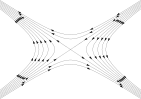
\includegraphics[width=.4\linewidth]{./pics/chap11-4-I.pdf}\quad
  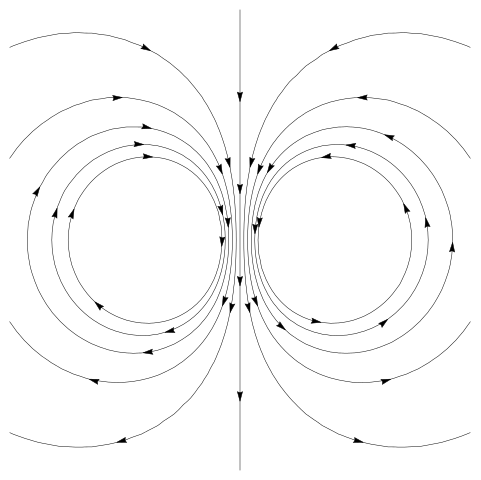
\includegraphics[width=.4\linewidth]{./pics/chap11-4-II.pdf}
  \caption{Figure 4}
  \label{fig:11-4}
\end{figure}

Let $X$ be a smooth tangent vector field on Mn and let $p_0\in M^n$ be a zero. Let
\begin{align*}
  F = h_*(X_{|U})\in C^\infty(\RR^n, \RR^n)
\end{align*}

for a chart $(U, h)$ with $h(p_0) = 0$. If $D_0F:\RR^n\to\RR^n$ is an isomorphism, then
$p_0$ is said to be a non-degenerate singularity or zero\index{non-degenarate zero}. Note that by the inverse
function theorem $F$ is a local diffeomorphism around 0, such that 0 is an isolated
zero for $F$. Hence $p_0\in M^n$ is also an isolated zero for $X$.

\begin{lemma}\label{lemma:11-20}
  If $p_0$ is a non-degenerate singularity, then
  \begin{align*}
    \imath(X, p_0) = \R{sign}(\det D_0F)\in \{\pm 1\}.
  \end{align*}
\end{lemma}

\begin{proof}
  By shrinking $U$ we may assume that $h$ maps $U$ diffeomorphically onto an
open set $U_0\in\RR^n$, which is star-shaped around 0, and that $F$ is a diffeomorphism
from $U_0$ to an open set. As in the proof of Lemma \ref{lemma:11-18} we can define a homotopy
\begin{align*}
  G:U_0\times[0, 1]\to\RR^n; \qquad G(x, t) = \left\{\begin{aligned}
    & D_0F   && \text{ if } t = 0 \\
    & F(tx)/t && \text{ if } t\neq 0.
  \end{aligned}\right.
\end{align*}

where $G$ can be extended smoothly to an open set $W$ in $U_0\times \RR$ that contains
$U_0\times [0,1]$. Choose $p > 0$ so that $\rho D^n\sseq U_0$. We get a homotopy $\tilde{G}:
S^{n-1}\times[0, 1]\to S^{n-1}$,
\begin{align*}
  \tilde{G}(x, t) = G(\rho x, t)\big/ \|G(\rho x, t)\|.
\end{align*}

between the map $F_\rho$ in Definition \ref{def:11-16} and the analogous map $A_\rho$ with $A=D_0F$.
It follows from Corollary \ref{corollary:11-2} that
\begin{align*}
  \imath(X; p_0) = \imath(F; 0) 
  = \R{deg}(F_\rho) = \R{deg}A_\rho  
  = \imath(A; 0).
\end{align*}

The map $f_A:\RR^n-\{0\}\to \RR^n-\{0\}$ induced by $A$ operates on $H^{n-1}(\RR^n-\{0\})$ by 
multiplication by $\imath(X; p_0)$; cf. Lemma \ref{lemma:11-17}. The result follows from 
Lemma \ref{lemma:6-14}.
\end{proof}

\begin{definition}\label{def:11-21}
  Let $X$ be a smooth vector field on $M^n$, with only isolated
  singularities. For a compact set $R\sseq M$ we define the total index of $X$ over
  $R$ to be
  \begin{align*}
    \R{Index}(X; R) = \sum \imath(X; p)
  \end{align*}
  where the summation runs over the finite number of zeros $p\in R$ for $X$. If $M$ is
  compact we write Index $(X)$ instead of Index $(X; M)$.
\end{definition}

\begin{theorem}\label{theorem:11-22}
  Let $F\in C^\infty(U, \RR)$ be a vector field on an open set $U\sseq\RR^n$,
with only isolated zeros. Let $R\sseq U$ be a compact domain with smooth boundary
$\partial R$, and assume that $F(p)\neq 0$ for $p\in\partial R$. Then
\begin{align*}
  \R{Index}(F; R) = \R{deg}(f),
\end{align*}
where $f:\partial R\to S^{n-1}$ is the map $f(x) = F(x)/\|F(x)\|$.
\end{theorem}

\begin{proof}
  Let $p_1, \cdots, p_k$ be the zeros in $R$ for $F$, and choose disjoint closed balls
$D_j\sseq R-\partial R$, with centers $p_j$. Define
\begin{align*}
  f_j: \partial D_j \to S^{n-1}; \qquad f_j(x) = F(x)/\|F(x)\|.
\end{align*}

We apply Proposition \ref{prop:11-11} with $X = R-\cup_{j}\mrg{D}_j$. The boundary $\partial x$ 
is the disjoint union of aR and the $(n - 1)$-spheres $\partial D_1, \cdots, \partial D_k$. Here $\partial D_j$, 
considered as boundary component of $X$, has the opposite orientation to the one induced from $D_j$. 
Thus
\begin{align*}
  \R{deg}(f) + \sum_{j=1}^{k}{-\R{deg}(f_j)} = 0.
\end{align*}

Finally $\R{deg}(f_j) = \imath(F; p_j)$ by the definition of local index and Corollary \ref{corollary:11-3}.
\end{proof}

\begin{corollary}\label{corollary:11-23}
  In the situation of Theorem \ref{theorem:11-22}, $\R{Index}(F; R)$ depends only on
the restriction of $F$ to $\partial R$.
\end{corollary}

\begin{corollary}\label{corollary:11-24}
  In the situation of Theorem \ref{theorem:11-22}, suppose for every $p\in\partial R$ that
  the vector $F(p)$ points outward. Let $g:\partial R\to S^{n-1}$ be the Gauss map which to
  $p\in\partial R$ associates the outward pointing unit normal vector to $\partial R$. Then
  \begin{align*}
    \R{Index}(F; R) = \R{deg}(g).
  \end{align*}
\end{corollary}

\begin{proof}
  By Corollary \ref{corollary:11-2} it sufficies to show that $f$ and $g$ are homotopic. Since
  $f(p)$ and $g(p)$ belong to the same open half-space of $\RR^n$ , the desired homotopy
  can be defined by
  \begin{align*}
    \frac{(1-t)f(p) + tg(p)}{\|(1-t)f(p) + tg(p)\|}.\qquad (0\le t\le 1).
    \tag*{\qedsymbol}
  \end{align*}
\end{proof}

\begin{lemma}\label{lemma:11-25}
  Suppose $F\in C^\infty(\RR^n, \RR^N)$ has the origin as its only zero. Then
  there exists an $F\in C^\infty(\RR^n, \RR^N)$, with only non-degenerate zeros, that coincides
  with $F$ outside a compact set.
\end{lemma}

\begin{proof}
  We choose a function $\phi\in C^\infty(\RR^n, [0, 1])$ with 
  \begin{align*}
    \phi(x) = \left\{\begin{aligned}
      & 1 && \text{ if } \|x\|\le 1 \\
      & 0 && \text{ if } \|x\|\ge 2.
    \end{aligned}\right.
  \end{align*}
  We want to define $\tilde{F}(x) = F(x) - \phi(x)w$ for a suitable $w\in\RR^n$. 
  For $\|x\|> 2$ we have $\tilde{F}(x) = F(x)$. Set
  \begin{align*}
    c = \inf_{1\le \|x\|\le 2} \|F(x)\| > 0
  \end{align*}
  and choose $w<c$. For $1\le\|x\|\le 2, \|\tilde{F}(x)\|\ge c-\|w\|>0$. Thus all 
  zeros of $\tilde{F}$ belong to the open unit ball $D^n$. Since $\tilde{F}$ coincides with 
  $F-w$ on $\mrg{D}^n$ 
  \begin{align*}
    \tilde{F}^{-1}(0) = \mrg{D}^n\cap F^{-1}(w).
  \end{align*}
  We can pick $w$ as a regular value of $F$ with $\|w\|<c$ by Sard's theorem. Then
  $D_p\tilde{F} = D_pF$ will be invertible for all $p\in\tilde{F}^{-1}(0)$, and $P$ has 
  the desired properties.
\end{proof}

Note, by Corollary \ref{corollary:11-23}, that
\begin{align}
  \imath(F; 0) = \sum_{p\in \tilde{F}^{-1}(p)}^{}{\imath(\tilde{F}, p)}
\end{align}

Here is a picture of $F$ and $\tilde{F}$ in a simple case:
\begin{figure}[!htb]
  \centering
  \includegraphics[width=.4\linewidth]{./pics/chap11-5-I.pdf}\quad
  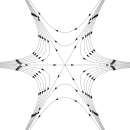
\includegraphics[width=.4\linewidth]{./pics/chap11-5-II.pdf}
  \caption{Figure 5(Left--$F$; Right--$\tilde{F}$)}
  \label{fig:11-5}
\end{figure}

The zero for $F$ of index -2 has been replaced by two non-degenerate zeros for
$\tilde{F}$, both of index -1.

\begin{corollary}\label{corollary:11-26}
  Let $X$ be a smooth vector field on the compact manifold $M^n$
with isolated singularities. Then there exists a smooth vector field $\tilde{X}$ on $M$ having
only non-degenerate zeros and with
\begin{align}\label{eq:11-14}
  \R{Index}(X) = \R{Index}(\tilde{X}).
\end{align}
\end{corollary}

\begin{proof}
  We choose disjoint coordinate patches which are diffeomorphic to $\RR^n$
around the finitely many zeros of $X$, and apply Lemma \ref{lemma:11-25} on the interior of
each of them to obtain $\tilde{X}$. The formula then follows from \eqref{eq:11-14}.
\end{proof}

\begin{theorem}\label{theorem:11-27}
  Let $M^n\sseq\RR^n$ be a compact smooth submanifold and let $N_\epsilon$ be
a tubular neighborhood of radius $\epsilon>0$ around $M$. Denote by $g:\partial N_\epsilon\to S^{n+k-1}$
the outward pointing Gauss map. If $X$ is an arbitrary smooth vector field on $M^n$
with isolated singularities, then
\begin{align*}
  \R{Index}(X) = \R{deg}(g).
\end{align*}
\end{theorem}

\begin{proof}
  By Corollary \ref{corollary:11-26} one may assume that $X$ only has non-degenerate zeros.
From the construction of the tubular neighborhood we have a smooth projection
$\pi: N\to M$ from an open tubular neighborhood $N$ with $N_\epsilon\sseq N\sseq \RR^{n+k}$, and 
can define a smooth vector field $F$ on $N$ by
\begin{align}\label{eq:11-15}
  F(q) = X(\pi(q)) + (q - \pi(q)).
\end{align}

ince the two summands are orthogonal, $F(q) = 0$ if and only if $q\in M$ and
$X(q) = 0$. For $q\in\partial N_\epsilon, q-\pi(q)$ is a vector normal to $T_q\partial N_\epsilon$ 
pointing outwards. Hence $X(\pi(q))\in T_q\partial N_\epsilon$ and $F(q)$ points outwards. 
By Corollary \ref{corollary:11-24} 
\begin{align*}
  \R{Index}(F; N) = \R{deg}(g).
\end{align*}

and it suffices to show that $\imath(X; p) = \imath(F; p)$ for an arbitrary zero of $X$. In 
local coordinates around $p$ in $M$, with $p$ corresponding to $0\in\RR^n$, $X$ can be written
in the form
\begin{align}\label{eq:11-16}
  X = \sum_{i=1}^{n}{f_i(x) \frac{\partial }{\partial x_i }},
\end{align}

where $f_i(0) = 0$, and by Lemma \ref{lemma:11-20} $\imath(X; p)$ is the sign of 
\begin{align}\label{eq:11-17}
  \det\left(\frac{\partial f_i }{\partial x_j }(0)\right).
\end{align}

By differentiating \eqref{eq:11-16} and substituting 0 one gets
\begin{align}\label{eq:11-18}
  \frac{\partial X }{\partial x_j }(0) 
  = \sum_{i=1 }^{n }{\frac{\partial f_i }{\partial x_j }(0) \frac{\partial }{\partial x_i }}.
\end{align}

It follows from \eqref{eq:11-15} that $D_pF:\RR^{n+k}\to\RR^{n+k}$ is the identity 
on $T_pM^\perp$ and by \eqref{eq:11-18} $D_pF$ maps $T_pM$ into itself by the linear map with 
matrix ($(\partial f_i/\partial x_i)(0)$) (with respect to the basis $(\partial/\partial x_i)_0$). 
It follows that $p$ is a non-degenerate zero for $F$ and that $\det D_pF$ has the same sign as 
the Jacobian in \eqref{eq:11-17}.
\end{proof}
\chapter{The Poincar\'{e}-Hopf Theorem }
\input{chapters/13-Poincare-Duality.tex}
\chapter{The Complex Projective Space \texorpdfstring{$\B{CP}^n$}{CPn}}
\chapter{Fiber Bundles and Vector Bundle}
\chapter{Operations on Vector Bundles and their Sections}
\input{chapters/17-Connections-and-Curvature.tex}
\chapter{Characteristic Classes of Complex Vector Bundles}
\input{chapters/19-The-Euler-Class.tex}
\chapter{Cohomology of Projective and Grassmannian Bundles}
\chapter{Thorn Isomorphism and the General Gauss-Bonnet Formula}


% Appendices
\setcounter{chapter}{0}
\def\thechapter{\Alph{chapter}}
\renewcommand\theHchapter{Appendix-\thechapter}
% appendices
\addtocontents{toc}{\def\protect\cftchappresnum{Appendix\ }}
\chapter{Smooth Partition of Unit}
The following technical theorem is a much used tool when working with smooth
maps and smooth manifolds.
For a function $f:U\to\RR$ with domain $U\subseteq\RR$ the support of $f$ in $U$ is the set
\begin{align*}
  \R{supp}_U(f) = \overline{\{x\in U\big| f(x)\neq 0\}}
\end{align*}

where the bar denotes the closure of the set in the induced topology on $U$. If $U$ is open 
in $\RR^n$ then $U-\R{supp}_U(d)$ is the largest open subset of $U$ on which $f$ vanishes.

\begin{theorem}\label{theorem:A.1}
  If $U\subseteq\RR^n$ is open and $\C{V} = (V_i)_{i\in I}$ is a cover of $U$ by open sets $V_i$, then there exists 
  smooth functions $\phi_i:U\to\ [0, 1]\; (i\in I)$, satisfying 
  \begin{enumerate}[(i)]
    \item $\R{supp}_U(\phi_i)\subseteq V_i$ for all $i\in I$.
    \item Every $x\in U$ has a neighborhood $W$ on which only finitely many $\phi_i$ do not vanish.
    \item For every $x\in U$ we have $\sum_{i\in I} \phi_i(x) = 1$.
  \end{enumerate}
  We say that $(\phi_i)_{i\in I}$ is a (smooth) partition of unity, which only is subordinate to the 
  cover $\C{V}$.
\end{theorem}

A family of functions $\phi_i:U\to\RR$ that satisfy (ii) is called locally finite. Note that
the sum $\sum_{i\in I}\phi_i$ in this case becomes a well-defined function $U\to\RR$. Moreover,
it is smooth when all the $\phi_i$ are smooth. The proof of Theorem \ref{theorem:A.1} requires
some preparations.


\begin{lemma}\label{lemma:A.7}
  If $A\in\RR^n$ is closed and $U\sseq\RR^n$ is open with $A\sseq U$, then there exists 
  a smooth function $\psi:\RR^n\to [0, 1]$ with $\supp_{\RR^n}(\psi)\sseq U$ and $\psi(x)=1$
  for $x\in A$.
\end{lemma}

\begin{proof}
  Apply Theorem \ref{theorem:A.1} to the cover of $\RR^n$ consisting of the open sets $V_1=U$
and $V_2 = \RR^n - A$. Now $\psi = \phi_1$ has the desired properties.
\end{proof}

\begin{lemma}\label{lemma:A.9}
  Suppose that $A\sseq U_0\sseq U\sseq \RR^n$, where $U_0$ and $U$ are open in
$\RR^n$ and $A$ is closed in $U$ (in the induced topology from $\RR^n$). Let $h:U\to W$ be
a continuous map to an open set $W\sseq\RR^m$ with smooth restriction to $U_0$. For
any continuous function $\epsilon:U\to (0, \infty)$ there exists a smooth map $f:U\to W$ that
satisfies
\begin{enumerate}[(i)]
  \item $\|f(x)-h(x)\|\le \epsilon(x)$ for all $x\in U$.
  \item $f(x) = h(x)$ for all $x\in A$.
\end{enumerate}
\end{lemma}

\begin{proof}
  If $W\neq \RR^m$ then $\epsilon(x)$ can be replaced by  
  \begin{align*}
    \epsilon_1(x) = \min(\epsilon(x), \frac12\dd(h(x), \RR^n-W))
  \end{align*}
  where $\dd(y, \RR^n-W) = \inf\{\|y-z\|\big| z\in\RR^n-W\}$. If $f:U\to W$ satisfies (i) with 
  $\epsilon_1$ instead of $\epsilon$, we will automatically get $f(U)\sseq W$. Hence, without loas of generality,
  we may assume that $W = \RR^m$.
  
  Using the continuity of $h$ and $\epsilon$, we can find for each $p\in U-A$ an open set 
  $U_p$ with $p\in U_p\sseq U-A$, such that $\|h(x) - h(p)\|\le \epsilon(x)$ for all $x\in U_p$.
  Apply Theorem \ref{theorem:A.1} to the open cover of $U$ consisting of the sets $U_0$ and $U_p, p\in U-A$.
  This yields smooth functions $\phi_0$ and $\phi_p$ from $U$ into $[0,1]$, which satisfy Theorem
  \ref{theorem:A.1}.(i), (ii) and (iii). By local finiteness, smoothness of $h$ on $U_0$ and the property
  $\supp_U(\phi_0) \sseq U_0$, we can define a smooth function $f:U\to\RR^m$ by
  \begin{align*}
    f(x) = \phi_0(x)h(x) + \sum_{p\in U-A}\phi_p(x)h(p).
  \end{align*}
  From Theorem \ref{theorem:A.1}.(iii) one obtain $h(x) = \phi_0(x)h(x) + \sum_{p\in U-A}\phi_p(x)h(p)$ and 
  thus 
  \begin{align*}
    f(x) - h(x) = \sum_{p\in U-A}\phi_p(x)(h(p)-h(x)).
  \end{align*}
  Now (ii) of the lemma follows because $\R{Supp}(\phi_p)\sseq U_p\sseq U-A$, and (i) follows from the calculation
  \begin{align*}
    \|f(x) - h(x)\|
      & \le \sum_{p\in U-A}\phi_p(x)\|h(p)-h(x)\|
        = \sum_{p\in U-A, x\in U_p}\phi_p(x)\|h(p)-h(x)\| \\
      & \le \sum_{}^{}{\phi_p(x)\epsilon(x)} 
        = \left(\sum_{}^{}{\phi_p(x)}\right)\cdot \epsilon(x)
        \le \epsilon(x).
  \end{align*}
\end{proof}
\input{chapters/App-B-Invariant-Polynomials.tex}
\chapter{Proof of Lemmas 12.12 and 12.13}
\chapter{Exercises}
\newcounter{exercise}
\setcounter{exercise}{1}
\newcommand{\newchap}{\stepcounter{exercise}\setcounter{enumi}{0}}


\begin{enumerate}[\theexercise.1.]
  \item Perform the calculations of Theorem \ref{theorem:1-6}.
  \item Let $W\subseteq\RR^3$ be the open set 
    \begin{align*}
      W = \{(x_1, x_2, x_3)\in\RR^3\big| \text{ either } x_3\neq 0 \text{ or } x_1^2 + x_2^2<1\}.
    \end{align*}
    Prove the existence and uniqueness of a function $f\in C^\infty(W, \RR)$ such that
    $\grad(F)$ is the vector field considered in Example \ref{example:1-8} and $F(0)= 0$.
    Find a simple expression for $F$ valid when $x_1^2 + x_2^2 < 1$. ( Hint: First note that $F$ is 
    constant on the open disc in the $x_l, x_2$-plane bounded by the unit circle $S$. Then integrate 
    along lines parallel to the $x_3$-axis.) \newchap
  \item Prov the formula in Remark \ref{remark:2-10}.
  \item Find an $\omega\in\alt^2\RR^4$ such that $\omega\wedge\omega\neq 0$.
  \item Show that there exist isomorphisms
    \begin{align*}
      \RR^3 \xra[i] \alt^1\RR^3, && \RR^3 \xra[j]\alt^2\RR^3 
    \end{align*}
    given by 
    \begin{align*}
      i(v)(w) = \langle v, w \rangle, && j(v)(w_1, w_2) = \det(v, w_1, w_2)
    \end{align*}
    where $\langle , \rangle$ is the usual inner product. Show that for $v_1, v_2\in\RR^2$, we have 
    \begin{align*}
      i(v_1)\wedge i(v_2) = j(v_1\times v_2).
    \end{align*}
  \item ... \setcounter{exercise}{7}\setcounter{enumi}{0}
  \item Show that $\RR^n$ does not contain a subset homeomorphic to $D^m$ when $m > n$.
  \item \label{exercise:7-2} Let $\Sigma\subseteq\RR^n$ be homeomorphic 
    to $S^k\; (1\le k\le n-2)$. Show that 
    \begin{align*}
      H^p(\RR^n-\Sigma) \simee \left\{\begin{aligned}
        & \RR && \text{ for } p=0, n-k-1, n-1 \\
        & 0 && \text{ otherwise }.
      \end{aligned}\right.
    \end{align*}
  \item Show that there is no continuous map $g:D^n\to S^{n-1}$ with $g|_{S^{n-1}}\sime \id|_{S^{n-1}}$.
  \item ... \setcounter{exercise}{9}\setcounter{enumi}{0}
  \item \label{exercise:9-1} Let $M\sseq\RR^l$ be a differentiable submanifold and assume the points 
    $p\in \RR^l$ and $p_0\in M$ are such that $\|p-p_0\|\le \|p-q\|$ for all $q\in M$. Show that 
    $p-p_0\in T_{p_0}M^\perp$.
  \item A smooth map $\varphi:M^m\to N^n$ between smooth manifolds is called immersive at $p\in M$, when 
    \begin{align*}
      D_p\varphi:T_pM\to T_{q}N, \qquad q\in\varphi(p)
    \end{align*}
    is injective. Show that there exists smooth charts $(U, h)$ in $M$ with $p\in U$, $h(p)=0$, and 
    $(V, k)$ in $N$ with $q\in V$, $k(q)=0$ such that 
    \begin{align*}
      k\circ\varphi\circ h^{-1}(x_1, \cdots, x_m) = (x_1, \cdots, x_m, 0, \cdots, 0).
    \end{align*}
    in a neighborhood of 0.\par
    (Hint: Reduce the problem to the case where $\varphi:W\to\RR^n$ is on an open neighborhood $W$ in $\RR^n$
    of 0 with $\varphi(0) = 0$, and 
    \begin{align*}
      \left(\frac{\partial \varphi_i(0)}{\partial x_j}\right)_{1\le i,j\le m}
    \end{align*}
    is an invertiable $m\times m$ matrix. Apply the inverse function theorem to 
    \begin{align*}
      F:W\times \RR^{n-m}\to&\RR^n;\\
      F(x_1, \cdots, x_n) 
        = (
            \varphi_1(x_1, \cdots, x_m), 
            \cdots, 
            & \varphi_m(x_1, \cdots, x_m), 
            x_{m+1}, 
            \cdots, 
            x_n
            ).)
    \end{align*}
  \item ... 
\end{enumerate}


% references and index
% references
\addtocontents{toc}{\def\protect\cftchappresnum{}}
\phantomsection
\addcontentsline{toc}{chapter}{References}
\nocite{*}
\printbibliography
% index
\phantomsection
\addcontentsline{toc}{chapter}{Index}
\printindex
\end{document}